\documentclass[11pt,a4paper]{article}

% ========================================
% PACKAGES
% ========================================
\usepackage[utf8]{inputenc}
\usepackage[T1]{fontenc}
\usepackage{lmodern}  % Better font support for larger sizes
\usepackage[english]{babel}  % Change to your language
\usepackage[margin=2.5cm]{geometry}

% Mathematics
\usepackage{amsmath, amssymb, amsthm}
\usepackage{mathtools}

% Graphics and colors
\usepackage{graphicx}
\usepackage{xcolor}
\usepackage{tikz}
\usetikzlibrary{positioning, arrows.meta, shapes.geometric, calc}
\usepackage{pgfplots}
\pgfplotsset{compat=1.18}
\usepackage[most]{tcolorbox}

% Lists and formatting
\usepackage{enumitem}
\usepackage{parskip}
\usepackage{fancyhdr}

% Code listings (if needed)
\usepackage{listings}
\usepackage{algorithm}
\usepackage{algorithmic}

% Hyperlinks
\usepackage{hyperref}
\hypersetup{
    colorlinks=true,
    linkcolor=blue,
    urlcolor=blue,
    citecolor=blue
}

% ========================================
% THEOREM ENVIRONMENTS
% ========================================
\theoremstyle{definition}
\newtheorem{definition}{Definition}[section]
\newtheorem{example}{Example}[section]
\newtheorem{exercise}{Exercise}[section]

\theoremstyle{plain}
\newtheorem{theorem}{Theorem}[section]
\newtheorem{lemma}[theorem]{Lemma}
\newtheorem{proposition}[theorem]{Proposition}
\newtheorem{corollary}[theorem]{Corollary}

\theoremstyle{remark}
\newtheorem*{remark}{Note}
\newtheorem*{observation}{Observation}

% ========================================
% CUSTOM COMMANDS
% ========================================
\newcommand{\R}{\mathbb{R}}
\newcommand{\N}{\mathbb{N}}
\newcommand{\Z}{\mathbb{Z}}
\newcommand{\Q}{\mathbb{Q}}
\newcommand{\C}{\mathbb{C}}

% ========================================
% TABLE OF CONTENTS DEPTH
% ========================================
\setcounter{tocdepth}{2} % Show only parts, sections, and subsections

% ========================================
% HEADER AND FOOTER
% ========================================
\setlength{\headheight}{14pt}
\pagestyle{fancy}
\fancyhf{}
\lhead{\leftmark}
\rhead{AR}
\cfoot{\thepage}
\renewcommand{\sectionmark}[1]{\markboth{#1}{}}

% ========================================
% DOCUMENT INFORMATION
% ========================================
\title{\textbf{Automated Reasoning}\\
\large Artificial Intelligence}
\author{Jacopo Parretti}
\date{I Semester 2025-2026}

% ========================================
% DOCUMENT
% ========================================
\begin{document}

% Custom title page
\begin{titlepage}
    \begin{center}
        \vspace*{2cm}
        
        % University/Course info at top
        {\large\textsc{Artificial Intelligence}}
        
        \vspace{0.4cm}
        \textcolor{blue!60!black}{\rule{0.5\textwidth}{1pt}}
        
        \vspace{2.5cm}
        
        % Main title with modern spacing
        {\fontsize{36}{44}\selectfont\bfseries Automated\\[0.5cm] Reasoning}
        
        \vspace{1.5cm}
        
        % Subtitle with clean design
        \begin{tcolorbox}[
            colback=blue!3!white,
            colframe=blue!40!black,
            width=0.6\textwidth,
            arc=1mm,
            boxrule=0.8pt,
            left=15pt,
            right=15pt,
            top=10pt,
            bottom=10pt
        ]
            \centering
            {\large\textit{Lecture Notes}}\\[0.3cm]
            \textcolor{gray}{Master's Program in Artificial Intelligence}
        \end{tcolorbox}
        
        \vfill
        
        % Clean course details
        \begin{tcolorbox}[
            enhanced,
            colback=white,
            colframe=gray!30,
            width=0.5\textwidth,
            arc=0mm,
            boxrule=0.5pt,
            left=20pt,
            right=20pt,
            top=12pt,
            bottom=12pt,
            shadow={2mm}{-2mm}{0mm}{black!10}
        ]
            \centering
            {\small\textcolor{gray!70}{\textbf{ACADEMIC YEAR}}}\\[0.4cm]
            {\Large 2025--2026}
        \end{tcolorbox}
        
        \vspace{2cm}
        
        % Author
        {\LARGE\textsc{Jacopo Parretti}}
        
        \vspace{1.5cm}
        
    \end{center}
\end{titlepage}

\newpage
\tableofcontents
\newpage

\part{}


\section{Introduction}

\subsection{Why Study Automated Reasoning?}

Automated Reasoning is a fundamental field of artificial intelligence concerned with the design and implementation of computational procedures that enable machines to solve problems formulated in logical languages. These procedures involve \textbf{logical inference and search}, allowing systems to reason in a deductive manner through mechanical processes.

Since the inception of artificial intelligence at the Dartmouth Conference in 1956, one of the core challenges has been to demonstrate machine intelligence through the automated proving of mathematical and logical theorems. This capability represents a cornerstone of symbolic AI, where knowledge is represented symbolically and stored in computer memory, and systematic procedures are applied to solve complex problems.

\textbf{Theorem proving} traditionally requires human-level mathematical reasoning and insight. The goal of automated reasoning is to mechanize this process, creating algorithms and systems capable of performing logical deduction without human intervention.

A logical language consists of formal symbols and syntactic rules. Within the symbolic approach to artificial intelligence, knowledge is encoded using these symbols, which are stored in computer memory. The system then applies a sequence of mechanical steps to manipulate these symbols and arrive at solutions to the given problems.



\newpage

\section{Historical Foundations and Theoretical Limits}

\subsection{The Hilbert-Turing Perspective}

The foundations of automated reasoning can be traced to fundamental questions in mathematical logic and computability. Since Alan Turing's seminal work on \textit{Turing machines} in 1936, researchers have pursued David Hilbert's 1900 challenge: is it possible to develop a mechanical procedure---executed deterministically by a human computor---capable of solving any mathematical problem?

\textbf{The Entscheidungsproblem}: A central question that emerged from this pursuit asks whether it is possible to define a mechanical method to determine the validity of formulas in first-order logic.

Turing demonstrated that the halting problem is undecidable using Turing machines. This fundamental result can be reduced to the validity problem in first-order logic, providing a negative answer to Hilbert's challenge. This undecidability result forms one of the core theoretical foundations of automated reasoning, establishing fundamental limits on what can be mechanically computed.

\subsection{Practical Applications of Automated Reasoning}

Automated reasoning systems find application across multiple domains requiring formal verification and systematic problem-solving:

\begin{itemize}
    \item \textbf{Planning}: Given an initial state, goal state, and formal model of agent actions, determine a sequence of moves that transforms the initial state into the goal state (utilizing SAT solvers)
    \item \textbf{Scheduling}: Generate temporal arrangements of tasks that satisfy complex temporal and resource constraints
    \item \textbf{Software Analysis and Verification}: Formal methods for ensuring program correctness, including:
        \begin{itemize}
            \item Provable privacy guarantees in security protocols
            \item Verification of distributed algorithms
            \item Analysis of randomized algorithms and their probabilistic properties
        \end{itemize}
    \item \textbf{Hybrid Approaches}: Integration of automated reasoning with machine learning techniques for enhanced problem-solving capabilities
\end{itemize}

These applications demonstrate the practical utility of automated reasoning in solving complex real-world problems that require rigorous logical analysis and systematic exploration of solution spaces.


\section{Core Problems in Automated Reasoning}

Automated reasoning fundamentally addresses three interconnected classes of decision problems in mathematical logic, each representing a distinct challenge in determining the truth properties of logical formulas.

\begin{center}
\textbf{\underline{The Three Core Problems in Automated Reasoning}}
\end{center}

\textbf{1. Satisfiability (SAT)}: Does there exist a model?

\textbf{2. Validity}: Is the formula true in all models?

\textbf{3. Logical Consequence}: Does the conclusion follow from premises?

\subsection{Satisfiability Problems}

A satisfiability problem (SAT) concerns determining whether a given logical formula has a truth assignment that makes it true. Formally, for a formula $\phi$ with free variables, we seek to determine if there exists an interpretation $\mathcal{I}$ such that $\mathcal{I} \models \phi$. This represents the existence problem---does there exist a model making the formula true?

\subsection{Validity Problems}

In contrast to satisfiability, validity problems ask whether a formula holds true under all possible interpretations. A formula $\phi$ is valid (denoted $\models \phi$) if every possible truth assignment to its variables results in $\phi$ evaluating to true. This corresponds to the universal quantification over all possible models---the formula must hold in every conceivable scenario.

\subsection{Logical Consequence Problems}

The logical consequence problem represents a generalization of validity, asking whether a conclusion necessarily follows from given premises. Given a set of assumptions $\Gamma = \{\phi_1, \phi_2, \dots, \phi_n\}$ and a conjecture $\psi$, we determine if $\Gamma \models \psi$ (i.e., if $\psi$ is true in every model where all formulas in $\Gamma$ are true). This captures the essence of logical deduction---what conclusions are forced by the given information.

These three problems form the foundation of automated reasoning systems, with satisfiability serving as the most tractable and finding widespread application in practical problem-solving contexts. 


\section{Formal Language and Semantics}

\subsection{Logical Language: First-Order Logic}

The formal language employed in automated reasoning is first-order logic (FOL), a substantial extension of propositional logic that incorporates quantification over individual elements.

\begin{center}
\textit{\underline{First-Order Logic Components}}
\end{center}

\textit{First-order logic achieves greater expressive power by introducing:}
\begin{itemize}
    \item \textit{Individual variables} ranging over domain elements
    \item \textit{Function symbols} for constructing complex terms
    \item \textit{Predicate symbols} for expressing relations between elements
    \item \textit{Quantifiers} ($\forall$, $\exists$) enabling statements about all or some elements
\end{itemize}

This enhanced expressiveness allows first-order logic to formalize mathematical structures, relationships, and properties in a manner impossible in propositional logic, which can only express truth-functional combinations of atomic propositions.

\subsection{Signature and Universe of Discourse}

A signature $\Sigma$ provides the vocabulary for interpreting formulas within a specific domain. Formally, a signature is a triple $\Sigma = \langle S, \mathcal{F}, \mathcal{P} \rangle$ where:

\begin{itemize}
    \item $S$ is a set of sorts (disjoint domains of interpretation)
    \item $\mathcal{F}$ is a set of function symbols, each with an arity specifying the number of arguments
    \item $\mathcal{P}$ is a set of predicate symbols, which we use to write formulas, each with an associated arity
\end{itemize}

The signature defines the syntactic elements available for constructing formulas, while the universe of discourse (or domain) provides the semantic interpretation. Sorts correspond to types in programming languages, enabling the formal specification of heterogeneous domains with different categories of objects.

The signature $\Sigma = \langle S, \mathcal{F}, \mathcal{P} \rangle$ can be further decomposed to provide a complete syntactic framework. The set of function symbols $\mathcal{F}$ is typically partitioned into two distinct subsets:

\begin{itemize}
    \item \textbf{Constant symbols} $C \subseteq \mathcal{F}$: These are function symbols of arity 0, representing named individuals in the domain. Constants have fixed interpretations and serve as proper names for specific domain elements.

    \item \textbf{Proper function symbols} $\mathcal{F} \setminus C$: These represent actual functions mapping tuples of domain elements to domain elements, each with arity $n \geq 1$.
\end{itemize}

Formally, a function symbol $f \in \mathcal{F}$ has type $s_1 \times s_2 \times \cdots \times s_n \rightarrow s$, where $s_1, \dots, s_n, s \in S$ are sorts indicating the domain and codomain of the function. For example:
\begin{itemize}
    \item $c : \rightarrow \texttt{int}$ (a constant symbol denoting a specific integer)
    \item $p : \rightarrow \texttt{color}$ (a constant symbol denoting a specific color)
    \item $f : \texttt{int} \times \texttt{int} \rightarrow \texttt{int}$ (a binary function like addition)
\end{itemize}

This decomposition enables precise specification of both individual elements (via constants) and functional relationships (via proper function symbols) within the formal language.

The complete signature structure $\langle S, C \cup (\mathcal{F} \setminus C) \cup \mathcal{P} \rangle$ provides the full syntactic foundation for expressing complex logical statements about structured domains.

Constants can be viewed as function symbols of arity 0---functions that require no arguments and directly denote specific domain elements. Additionally, to construct quantified formulas and express generality, we require a countably infinite set of variables $X = \{x, y, z, \dots\}$ disjoint from the signature symbols. 


Thus, the function symbols may be comprehensively categorized as $\mathcal{F} = C \cup (\mathcal{F} \setminus C) \cup \mathcal{P}$, where $\mathcal{P}$ represents the set of predicate symbols. Each predicate symbol $p \in \mathcal{P}$ has arity $n \geq 0$ and type $s_1 \times s_2 \times \cdots \times s_n$, where the final sort represents the truth value (typically a boolean sort).

Predicate symbols differ fundamentally from function symbols in that they represent relations rather than functions---they evaluate to truth values rather than domain elements. For example:
\begin{itemize}
    \item $even : \texttt{int} \rightarrow \texttt{bool}$ (unary predicate testing parity)
    \item $less : \texttt{int} \times \texttt{int} \rightarrow \texttt{bool}$ (binary relation for ordering)
\end{itemize}

The complete signature structure $\langle S, C \cup (\mathcal{F} \setminus C) \cup \mathcal{P} \rangle$ provides the full syntactic foundation for expressing complex logical statements about structured domains.

Constants can be viewed as function symbols of arity 0---functions that require no arguments and directly denote specific domain elements. Additionally, to construct quantified formulas and express generality, we require a countably infinite set of variables $X = \{x, y, z, \dots\}$ disjoint from the signature symbols.

\section{Syntactic Foundations: Terms and Formulas}

\subsection{Terms: The Building Blocks}

The most fundamental syntactic objects in first-order logic are \textbf{terms}, which represent individuals in the domain of discourse. The set of terms $\mathcal{T}_\Sigma(X)$ over signature $\Sigma$ and variables $X$ is inductively defined as the smallest set satisfying:

\begin{itemize}
    \item \textbf{Constants}: If $c \in C$ is a constant symbol, then $c \in \mathcal{T}_\Sigma(X)$
    \item \textbf{Variables}: If $x \in X$ is a variable, then $x \in \mathcal{T}_\Sigma(X)$
    \item \textbf{Function application}: If $f \in \mathcal{F}$ is a function symbol of arity $n \geq 1$ and $t_1, \dots, t_n \in \mathcal{T}_\Sigma(X)$ are terms, then $f(t_1, \dots, t_n) \in \mathcal{T}_\Sigma(X)$
\end{itemize}

Terms can be conceptualized as finite trees where:
\begin{itemize}
    \item Leaf nodes are constants or variables
    \item Internal nodes are function symbols applied to subterms
\end{itemize}

For example, the term $f(x, g(a), z)$ has the tree representation:
\[
\begin{array}{c}
  f \\
  | \\
  \begin{array}{ccc}
    x & g & z \\
       & | & \\
       & a &
  \end{array}
\end{array}
\]


Terms may contain subterms, which correspond to subtrees in this representation. Complex terms are constructed recursively from simpler subterms, reflecting the hierarchical nature of the syntactic structure.

\subsection{From Terms to Atomic Formulas}

Having established the notion of terms as representations of individuals, we now introduce atomic formulas to express relationships between these individuals. An \textbf{atomic formula} (or \textbf{atom}) is constructed by applying a predicate symbol to an appropriate number of terms.

Formally, if $P \in \mathcal{P}$ is a predicate symbol of arity $n \geq 0$ and $t_1, \dots, t_n \in \mathcal{T}_\Sigma(X)$ are terms, then $P(t_1, \dots, t_n)$ is an atomic formula. When $n = 0$, the atomic formula reduces to the predicate symbol itself $P$, which can be interpreted as a propositional constant.

The truth value of an atomic formula $P(t_1, \dots, t_n)$ depends on the interpretation of the predicate $P$ and the denotations of the terms $t_1, \dots, t_n$ in a given model.

\subsection{Literals: Positive and Negative Atomic Formulas}

A \textbf{literal} is either an atomic formula (positive literal) or its negation (negative literal). Formally, if $\phi$ is an atomic formula, then:
\begin{itemize}
    \item $\phi$ is a positive literal
    \item $\neg \phi$ is a negative literal
\end{itemize}

Literals represent the basic building blocks for constructing more complex logical formulas and play a crucial role in automated reasoning systems, particularly in resolution-based theorem proving.

\subsection{Logical Connectives}

Logical connectives provide the means to construct complex formulas from simpler ones. These operators enable the expression of compound logical statements through systematic combination of atomic formulas and literals.

The primary logical connectives include:
\begin{itemize}
    \item \textbf{Negation} ($\neg$): Expresses logical denial or contradiction
    \item \textbf{Conjunction} ($\wedge$): Represents logical conjunction (AND)
    \item \textbf{Disjunction} ($\vee$): Represents logical disjunction (OR)
    \item \textbf{Implication} ($\rightarrow$): Expresses logical implication (IF...THEN)
    \item \textbf{Biconditional} ($\leftrightarrow$): Represents logical equivalence (IF AND ONLY IF)
\end{itemize}

\subsection{Formulas: The Complete Syntax}

The set of \textbf{formulas} (or \textbf{well-formed formulas}) $\mathcal{F}_\Sigma(X)$ over signature $\Sigma$ and variables $X$ is inductively defined as the smallest set satisfying:

\begin{itemize}
    \item \textbf{Atomic formulas}: If $P \in \mathcal{P}$ is a predicate symbol of arity $n \geq 0$ and $t_1, \dots, t_n \in \mathcal{T}_\Sigma(X)$, then $P(t_1, \dots, t_n) \in \mathcal{F}_\Sigma(X)$

    \item \textbf{Negation}: If $\phi \in \mathcal{F}_\Sigma(X)$, then $(\neg \phi) \in \mathcal{F}_\Sigma(X)$

    \item \textbf{Binary connectives}: If $\phi, \psi \in \mathcal{F}_\Sigma(X)$, then:
        \begin{itemize}
            \item $(\phi \wedge \psi) \in \mathcal{F}_\Sigma(X)$ (conjunction)
            \item $(\phi \vee \psi) \in \mathcal{F}_\Sigma(X)$ (disjunction)
            \item $(\phi \rightarrow \psi) \in \mathcal{F}_\Sigma(X)$ (implication)
            \item $(\phi \leftrightarrow \psi) \in \mathcal{F}_\Sigma(X)$ (biconditional)
        \end{itemize}
\end{itemize}


This inductive definition ensures that all syntactically valid logical expressions can be systematically constructed from the basic building blocks of atomic formulas through the application of logical connectives.

\subsection{Quantifiers: Universality and Existence}

To complete the syntax of first-order logic, we introduce quantifiers that express generality and existence over the domain of discourse:

\begin{itemize}
    \item \textbf{Universal quantifier} ($\forall$): If $\phi \in \mathcal{F}_\Sigma(X)$ is a formula and $x \in X$ is a variable, then $(\forall x \, \phi) \in \mathcal{F}_\Sigma(X)$
    \item \textbf{Existential quantifier} ($\exists$): If $\phi \in \mathcal{F}_\Sigma(X)$ is a formula and $x \in X$ is a variable, then $(\exists x \, \phi) \in \mathcal{F}_\Sigma(X)$
\end{itemize}

Quantifiers bind variables within their scope, enabling the expression of properties that hold for all elements of the domain (universal quantification) or for at least one element (existential quantification).

\subsection{Illustrative Example: Geometric Axioms}

Consider the following first-order formula expressing that any two distinct points determine a unique line:

\[
\forall x \, \forall y \, \left( (P(x) \wedge P(y) \wedge x \neq y) \rightarrow \exists z \, (L(z) \wedge Q(z, x, y) \wedge \forall w \, (L(w) \wedge Q(w, x, y) \rightarrow w = z)) \right)
\]

Where:
\begin{itemize}
    \item $P(x)$ denotes that $x$ is a point
    \item $L(z)$ denotes that $z$ is a line
    \item $Q(z, x, y)$ denotes that line $z$ passes through points $x$ and $y$
    \item $x \neq y$ expresses that points $x$ and $y$ are distinct
\end{itemize}


This axiom formalizes the geometric principle that given any two distinct points in space, there exists exactly one line passing through both points, capturing a fundamental property of Euclidean geometry within the framework of first-order logic.

\subsection{Closed Formulas and Variable Scope}

A \textbf{closed formula} (or \textbf{sentence}) is a formula containing no free variables---all variables are bound by quantifiers. A variable is \textbf{free} in a formula if it appears outside the scope of any quantifier that binds it; conversely, a variable is \textbf{bound} if it appears within the scope of a quantifier.

Formulas may contain both free and bound occurrences of variables. For proper semantic interpretation, variables must be \textbf{standardized apart}, meaning that no variable appears both free and bound in the same formula, and distinct quantifiers use distinct bound variables.



\newpage

\part{Semantic Foundations}

\section{Interpretations and Models}

\subsection{The Concept of Interpretation}

To assign meaning to syntactic formulas in first-order logic, we require a formal notion of \textbf{interpretation}. An interpretation $\mathcal{I}$ provides a semantic mapping from the syntactic elements of a signature to concrete mathematical objects.

\begin{tcolorbox}[colback=purple!5!white,colframe=purple!75!black,title=\textbf{Interpretation Components}]
In the unsorted case, an interpretation consists of:
\begin{itemize}
    \item A non-empty set $D$ called the \textbf{domain} (or universe of discourse)
    \item An interpretation function $\Phi$ that maps:
    \begin{itemize}
        \item Each predicate symbol $P \in \mathcal{P}$ of arity $n$ to a subset $\Phi(P) \subseteq D^n$ (representing an $n$-ary relation over the domain)
        \item Each function symbol $f \in \mathcal{F}$ of arity $n$ to a function $\Phi(f) : D^n \rightarrow D$
        \item Each constant symbol $c \in C$ to a specific element $\Phi(c) \in D$
    \end{itemize}
\end{itemize}
\end{tcolorbox}

The interpretation function $\Phi$ bridges the gap between syntax and semantics, transforming abstract symbols into concrete mathematical entities.

\subsection{Example: Interpreting a Formula over Natural Numbers}

Consider the first-order formula:
\[
\forall x \, (\neg P(x) \rightarrow P(f(x)))
\]

This formula contains:
\begin{itemize}
    \item A unary predicate symbol $P$
    \item A unary function symbol $f$
    \item A universally quantified variable $x$
\end{itemize}

Since the formula is closed (contains no free variables), its truth value depends entirely on the chosen interpretation.

\textbf{Constructing an interpretation}: Let us define an interpretation $\mathcal{I} = \langle D, \Phi \rangle$ where:
\begin{itemize}
    \item \textbf{Domain}: $D = \N$ (the set of natural numbers)
    \item \textbf{Function interpretation}: $\Phi(f) : \N \rightarrow \N$ is the successor function, defined by $\Phi(f)(n) = n + 1$ for all $n \in \N$
    \item \textbf{Predicate interpretation}: $\Phi(P) = \{0, 2, 4, 6, \dots\} = \{2k \mid k \in \N\}$ (the set of even natural numbers)
\end{itemize}

\subsection{Semantic Evaluation}

Under this interpretation $\mathcal{I}$, the formula $\forall x \, (\neg P(x) \rightarrow P(f(x)))$ receives the following semantic reading:

\textit{For all natural numbers $x$, if $x$ is not even, then the successor of $x$ is even.}

To determine whether this formula is true in interpretation $\mathcal{I}$, we must verify whether the implication holds for every element of the domain:
\begin{itemize}
    \item If $x$ is odd (i.e., $x \notin \Phi(P)$), then $x + 1$ must be even (i.e., $x + 1 \in \Phi(P)$)
\end{itemize}

This statement is indeed true in the natural numbers: the successor of any odd number is even. Therefore, the formula is \textbf{satisfied} by interpretation $\mathcal{I}$, and we write $\mathcal{I} \models \forall x \, (\neg P(x) \rightarrow P(f(x)))$.

\subsection{Formal Verification of Satisfaction}

To formally verify that $\mathcal{I} \models \forall x \, (\neg P(x) \rightarrow P(f(x)))$, we must check that for all $n \in \N$, the interpretation satisfies the implication with the substitution $\{x \leftarrow n\}$.

By the semantics of implication, $\mathcal{I}$ satisfies $(\neg P(x) \rightarrow P(f(x)))$ with assignment $\{x \leftarrow n\}$ if and only if:
\begin{itemize}
    \item Either $\mathcal{I}$ does not satisfy $\neg P(x)$ with $\{x \leftarrow n\}$ (i.e., $\mathcal{I}$ satisfies $P(x)$ with $\{x \leftarrow n\}$), or
    \item $\mathcal{I}$ satisfies $P(f(x))$ with $\{x \leftarrow n\}$
\end{itemize}

Equivalently, for all $n \in \N$, either $n \in \Phi(P)$ or $\Phi(f)(n) \in \Phi(P)$.

\textbf{Truth condition for atomic formulas}: An atomic formula $P(t)$ is true under interpretation $\mathcal{I}$ if and only if the interpretation of the term $t$ belongs to the interpretation of the predicate $\Phi(P)$.

In our example, for all $n \in \N$:
\begin{itemize}
    \item Either $n \in \Phi(P)$ (meaning $n$ is even), or
    \item $\Phi(f)(n) = n + 1 \in \Phi(P)$ (meaning the successor of $n$ is even)
\end{itemize}

This condition holds for all natural numbers, confirming that the formula is satisfied by the interpretation.

\subsection{Formal Definition of Interpretation}

Having illustrated the concept through examples, we now provide the complete formal definition of an interpretation in first-order logic.

An \textbf{interpretation} $\mathcal{I}$ consists of a triple $\mathcal{I} = \langle D, \Phi, \beta \rangle$ where:

\begin{itemize}
    \item \textbf{Domain}: $D$ is a non-empty set representing the universe of discourse
    
    \item \textbf{Interpretation function} $\Phi$ maps signature symbols to semantic objects:
    \begin{itemize}
        \item For each constant symbol $c \in C$: $\Phi(c) = d \in D$
        \item For each function symbol $f \in \mathcal{F}$ of arity $n \geq 1$: $\Phi(f) : D^n \rightarrow D$, where $D^n$ denotes the $n$-fold Cartesian product $D \times D \times \cdots \times D$
        \item For each predicate symbol $P \in \mathcal{P}$ of arity $n \geq 0$: $\Phi(P) \subseteq D^n$ (an $n$-ary relation over $D$)
    \end{itemize}
    
    \item \textbf{Variable assignment} $\beta$ maps each variable to a domain element:
    \begin{itemize}
        \item $\beta : X \rightarrow D$ such that $\beta(x) = d \in D$ for all variables $x \in X$
    \end{itemize}
\end{itemize}

\textbf{Assignment update notation}: Given an assignment $\beta$ and a substitution $x \leftarrow d$, we define the updated assignment $\beta[x \leftarrow d]$ as:
\[
\beta[x \leftarrow d](y) = 
\begin{cases}
d & \text{if } y = x \\
\beta(y) & \text{otherwise}
\end{cases}
\]

This notation allows us to formally express the evaluation of formulas with different variable bindings, which is essential for defining the semantics of quantified formulas.






\section{Satisfaction Relation}

\subsection{The Satisfaction Relation}

Having defined interpretations and variable assignments, we now formalize the central semantic concept: when does an interpretation \textbf{satisfy} a formula? The satisfaction relation, denoted $\mathcal{I} \models_\beta \phi$, specifies the conditions under which a formula $\phi$ is true in interpretation $\mathcal{I}$ with variable assignment $\beta$.

Let $F$ and $G$ denote arbitrary formulas. The satisfaction relation is defined inductively on the structure of formulas.

\subsection{Interpretation of Terms}

Before defining satisfaction for formulas, we must specify how terms are interpreted. Given an interpretation $\mathcal{I} = \langle D, \Phi, \beta \rangle$, the interpretation of a term $t$, denoted $\Phi_\beta(t)$, is defined recursively:

\begin{itemize}
    \item \textbf{Constants}: $\Phi_\beta(c) = \Phi(c) \in D$
    \item \textbf{Variables}: $\Phi_\beta(x) = \beta(x) \in D$
    \item \textbf{Function application}: $\Phi_\beta(f(t_1, \dots, t_n)) = \Phi(f)(\Phi_\beta(t_1), \dots, \Phi_\beta(t_n)) \in D$
\end{itemize}

Each term evaluates to a specific element of the domain under a given interpretation.

\subsection{Satisfaction for Atomic Formulas}

\textbf{Base case} (atomic formulas): An interpretation $\mathcal{I}$ satisfies an atomic formula $P(t_1, \dots, t_n)$ under assignment $\beta$ if and only if the tuple of interpreted terms belongs to the interpretation of the predicate:

\[
\mathcal{I} \models_\beta P(t_1, \dots, t_n) \quad \text{iff} \quad (\Phi_\beta(t_1), \dots, \Phi_\beta(t_n)) \in \Phi(P)
\]

\subsection{Satisfaction for Logical Connectives}

The satisfaction relation extends to compound formulas through the following inductive clauses. Note that all satisfaction relations are parameterized by the variable assignment $\beta$, written as $\models_\beta$.

\begin{itemize}
    \item \textbf{Negation}: 
    \[
    \mathcal{I} \models_\beta \neg F \quad \text{iff} \quad \mathcal{I} \not\models_\beta F
    \]
    
    \item \textbf{Conjunction}: 
    \[
    \mathcal{I} \models_\beta (F \wedge G) \quad \text{iff} \quad \mathcal{I} \models_\beta F \text{ and } \mathcal{I} \models_\beta G
    \]
    
    \item \textbf{Disjunction}: 
    \[
    \mathcal{I} \models_\beta (F \vee G) \quad \text{iff} \quad \mathcal{I} \models_\beta F \text{ or } \mathcal{I} \models_\beta G
    \]
    
    \item \textbf{Implication}: 
    \[
    \mathcal{I} \models_\beta (F \rightarrow G) \quad \text{iff} \quad \mathcal{I} \not\models_\beta F \text{ or } \mathcal{I} \models_\beta G
    \]
    Equivalently: if $\mathcal{I} \models_\beta F$ then $\mathcal{I} \models_\beta G$
    
    \item \textbf{Biconditional}: 
    \[
    \mathcal{I} \models_\beta (F \leftrightarrow G) \quad \text{iff} \quad \mathcal{I} \models_\beta F \text{ if and only if } \mathcal{I} \models_\beta G
    \]
\end{itemize}

\subsection{Satisfaction for Quantified Formulas}

Quantifiers introduce variable bindings that range over the entire domain:

\begin{itemize}
    \item \textbf{Universal quantification}: 
    \[
    \mathcal{I} \models_\beta \forall x \, G \quad \text{iff} \quad \text{for all } d \in D, \, \mathcal{I} \models_{\beta[x \leftarrow d]} G
    \]
    The formula $\forall x \, G$ is satisfied if $G$ is satisfied under every possible assignment to $x$.
    
    \item \textbf{Existential quantification}: 
    \[
    \mathcal{I} \models_\beta \exists x \, G \quad \text{iff} \quad \text{there exists } d \in D \text{ such that } \mathcal{I} \models_{\beta[x \leftarrow d]} G
    \]
    The formula $\exists x \, G$ is satisfied if $G$ is satisfied under at least one assignment to $x$.
\end{itemize}

This completes the inductive definition of the satisfaction relation, providing a complete semantics for first-order logic.

\subsection{Example: Quantifier Evaluation}

Consider the formula $\forall x \, \exists y \, R(x, y)$, which can be read as "for all $x$, there exists $y$ such that $x < y$".

Let $\mathcal{I} = \langle \N, \Phi \rangle$ where $\Phi(R) = \{(n, m) \in \N \times \N \mid n < m\}$ (the standard ordering on natural numbers).

To verify $\mathcal{I} \models \forall x \, \exists y \, R(x, y)$, we apply the semantic definitions:
\begin{align*}
\mathcal{I} \models \forall x \, \exists y \, R(x, y) 
&\quad \text{iff} \quad \text{for all } n \in \N, \, \mathcal{I} \models_{\beta[x \leftarrow n]} \exists y \, R(x, y) \\
&\quad \text{iff} \quad \text{for all } n \in \N, \text{ there exists } m \in \N \text{ such that } \mathcal{I} \models_{\beta[x \leftarrow n, y \leftarrow m]} R(x, y) \\
&\quad \text{iff} \quad \text{for all } n \in \N, \text{ there exists } m \in \N \text{ such that } (n, m) \in \Phi(R) \\
&\quad \text{iff} \quad \text{for all } n \in \N, \text{ there exists } m \in \N \text{ such that } n < m
\end{align*}

This statement is \textbf{false} in $\N$ because there is no natural number greater than all natural numbers. However, it would be true in $\mathbb{Z}$ or $\mathbb{Q}$, demonstrating how truth depends on the chosen interpretation.

\section{Semantic Properties of Formulas}

Having established the satisfaction relation, we now define fundamental semantic properties that classify formulas according to their truth behavior across different interpretations.

\begin{tcolorbox}[colback=red!5!white,colframe=red!75!black,title=\textbf{Semantic Properties of Formulas}]
\subsection*{Satisfiability}
A formula $F$ is \textbf{satisfiable} if there exists an interpretation $\mathcal{I}$ such that $\mathcal{I} \models F$.
\[
F \text{ is satisfiable} \quad \Leftrightarrow \quad \exists \mathcal{I} : \mathcal{I} \models F
\]

\subsection*{Validity}
A formula $F$ is \textbf{valid} (or a \textbf{tautology}) if for all interpretations $\mathcal{I}$, we have $\mathcal{I} \models F$.
\[
F \text{ is valid} \quad \Leftrightarrow \quad \forall \mathcal{I} : \mathcal{I} \models F
\]

\subsection*{Unsatisfiability}
A formula $F$ is \textbf{unsatisfiable} if there exists no interpretation $\mathcal{I}$ such that $\mathcal{I} \models F$.
\[
F \text{ is unsatisfiable} \quad \Leftrightarrow \quad \nexists \mathcal{I} : \mathcal{I} \models F
\]

\subsection*{Invalidity}
A formula $F$ is \textbf{invalid} if there exists an interpretation $\mathcal{I}$ such that $\mathcal{I} \not\models F$.
\[
F \text{ is invalid} \quad \Leftrightarrow \quad \exists \mathcal{I} : \mathcal{I} \not\models F
\]
\end{tcolorbox}

\subsection{Satisfiability}

A formula $F$ is \textbf{satisfiable} if there exists an interpretation $\mathcal{I}$ such that $\mathcal{I} \models F$. In this case, we say that $\mathcal{I}$ is a \textbf{model} of $F$.

\subsection{Validity}

We denote validity by $\models F$.

\subsection{Unsatisfiability}

Unsatisfiable formulas are false in every interpretation.

\subsection{Invalidity}

In this case, we say that $\mathcal{I}$ is a \textbf{countermodel} (or \textbf{counterexample}) for $F$.

\subsection{Relationships Between Semantic Properties}

These semantic properties are intimately related through negation:

\begin{theorem}[Validity and Unsatisfiability]
A formula $F$ is valid if and only if $\neg F$ is unsatisfiable.
\end{theorem}

\begin{proof}
Suppose $F$ is valid. Then for all interpretations $\mathcal{I}$, we have $\mathcal{I} \models F$, which implies $\mathcal{I} \not\models \neg F$. Therefore, $\neg F$ is unsatisfiable.

Conversely, if $\neg F$ is unsatisfiable, then for all interpretations $\mathcal{I}$, we have $\mathcal{I} \not\models \neg F$, which implies $\mathcal{I} \models F$. Therefore, $F$ is valid.
\end{proof}

\begin{theorem}[Satisfiability and Invalidity]
A formula $F$ is satisfiable if and only if $\neg F$ is invalid.
\end{theorem}

\begin{proof}
$F$ is satisfiable if and only if there exists an interpretation $\mathcal{I}$ such that $\mathcal{I} \models F$, which is equivalent to $\mathcal{I} \not\models \neg F$. This is precisely the condition for $\neg F$ to be invalid.
\end{proof}

These relationships demonstrate the duality between validity and unsatisfiability, and between satisfiability and invalidity, providing a complete characterization of the semantic landscape of first-order logic.

\section{Logical Consequence}

\subsection{The Three Fundamental Query Types}

Automated reasoning systems must be capable of resolving three fundamental types of semantic queries:
\begin{enumerate}
    \item \textbf{Satisfiability queries}: Is formula $F$ satisfiable?
    \item \textbf{Validity queries}: Is formula $F$ valid?
    \item \textbf{Logical consequence queries}: Does $F$ follow logically from a set of hypotheses $H$?
\end{enumerate}

\subsection{Definition of Logical Consequence}

\begin{tcolorbox}[colback=cyan!5!white,colframe=cyan!75!black,title=\textbf{Logical Consequence}]
Let $H = \{\phi_1, \phi_2, \dots, \phi_n\}$ be a set of formulas (the \textbf{hypotheses} or \textbf{premises}) and let $F$ be a formula (the \textbf{conclusion}). We say that $F$ is a \textbf{logical consequence} of $H$, written $H \models F$, if:
\[
H \models F \quad \Leftrightarrow \quad \text{for all interpretations } \mathcal{I}, \text{ if } \mathcal{I} \models H \text{ then } \mathcal{I} \models F
\]
\end{tcolorbox}

In other words, $F$ is a logical consequence of $H$ if every model of $H$ is also a model of $F$. Here, $\mathcal{I} \models H$ means that $\mathcal{I}$ satisfies all formulas in $H$.

\subsection{The Deduction Theorem}

The deduction theorem establishes a fundamental connection between logical consequence and validity, reducing the problem of checking entailment to the problem of checking validity.

\begin{tcolorbox}[colback=teal!10!white,colframe=teal!75!black,title=\textbf{Deduction Theorem}]
\begin{theorem}[Deduction Theorem]
Let $H$ be a set of formulas and $F$ be a formula. Then:
\[
H \models F \quad \text{iff} \quad \models (H \rightarrow F)
\]
where $H \rightarrow F$ denotes the implication from the conjunction of all formulas in $H$ to $F$.
\end{theorem}
\end{tcolorbox}

\begin{proof}
We prove both directions:

\textbf{($\Rightarrow$)} Assume $H \models F$. We must show that $H \rightarrow F$ is valid, i.e., for all interpretations $\mathcal{I}$, we have $\mathcal{I} \models H \rightarrow F$.

Let $\mathcal{I}$ be an arbitrary interpretation. By the semantics of implication, $\mathcal{I} \models H \rightarrow F$ holds if either:
\begin{itemize}
    \item $\mathcal{I} \not\models H$ (the antecedent is false), or
    \item $\mathcal{I} \models F$ (the consequent is true)
\end{itemize}

If $\mathcal{I} \not\models H$, then $\mathcal{I} \models H \rightarrow F$ trivially. If $\mathcal{I} \models H$, then by the hypothesis $H \models F$, we have $\mathcal{I} \models F$, so $\mathcal{I} \models H \rightarrow F$. In both cases, $\mathcal{I} \models H \rightarrow F$.

\textbf{($\Leftarrow$)} Conversely, suppose $H \rightarrow F$ is valid. Then for all interpretations $\mathcal{I}$, we have $\mathcal{I} \models H \rightarrow F$. By the semantics of implication, for all $\mathcal{I}$, either $\mathcal{I} \not\models H$ or $\mathcal{I} \models F$. Therefore, for all $\mathcal{I}$ such that $\mathcal{I} \models H$, we must have $\mathcal{I} \models F$, which is precisely the definition of $H \models F$.
\end{proof}

\subsection{Notational Ambiguity of $\models$}

The symbol $\models$ is used in three distinct but related contexts:

\begin{itemize}
    \item \textbf{Satisfaction}: $\mathcal{I} \models F$ means interpretation $\mathcal{I}$ satisfies formula $F$
    \item \textbf{Validity}: $\models F$ means formula $F$ is valid (satisfied by all interpretations)
    \item \textbf{Entailment}: $H \models F$ means formula $F$ is a logical consequence of the set of formulas $H$
\end{itemize}

While this overloading may initially seem confusing, these three uses are semantically coherent and represent different aspects of the same fundamental semantic relation.

\subsection{Reduction to Unsatisfiability}

A fundamental result connects logical consequence to unsatisfiability, providing another characterization of entailment.

\begin{tcolorbox}[colback=yellow!10!white,colframe=yellow!75!black,title=\textbf{Key Theorem: Reduction to Unsatisfiability}]
\begin{theorem}[Logical Consequence via Unsatisfiability]
Let $H$ be a set of formulas and $F$ be a formula. Then:
\[
H \models F \quad \text{iff} \quad H \cup \{\neg F\} \text{ is unsatisfiable}
\]
\end{theorem}
\end{tcolorbox}

\begin{proof}
We prove both directions:

\textbf{($\Rightarrow$)} Assume $H \models F$. We must show that $H \cup \{\neg F\}$ is unsatisfiable.

Suppose for contradiction that there exists an interpretation $\mathcal{I}$ such that $\mathcal{I} \models H \cup \{\neg F\}$. Then $\mathcal{I} \models H$ and $\mathcal{I} \models \neg F$, which implies $\mathcal{I} \not\models F$. However, since $H \models F$ and $\mathcal{I} \models H$, we must have $\mathcal{I} \models F$, which is a contradiction. Therefore, $H \cup \{\neg F\}$ is unsatisfiable.

\textbf{($\Leftarrow$)} Assume $H \cup \{\neg F\}$ is unsatisfiable. We must show that $H \models F$.

Let $\mathcal{I}$ be any interpretation such that $\mathcal{I} \models H$. Since $H \cup \{\neg F\}$ is unsatisfiable, there is no interpretation that satisfies both $H$ and $\neg F$. Therefore, $\mathcal{I} \not\models \neg F$, which implies $\mathcal{I} \models F$. Since this holds for all interpretations satisfying $H$, we conclude that $H \models F$.
\end{proof}

\section{Refutational Reasoning}

\subsection{Proof by Contradiction}

\begin{tcolorbox}[colback=orange!10!white,colframe=orange!75!black,title=\textbf{Refutational Reasoning (Proof by Contradiction)}]
\textbf{Refutational reasoning} (or \textbf{proof by refutation}) is a fundamental technique in automated reasoning based on the principle of \textit{reductio ad absurdum}. To prove that a conclusion $F$ follows from hypotheses $H$, we assume the negation of the conclusion and derive a contradiction.

The method proceeds as follows:
\begin{enumerate}
    \item \textbf{Goal}: Prove $H \models F$ (where $H$ represents assumptions and $F$ represents the conjecture)
    \item \textbf{Method}: Show that $H \cup \{\neg F\}$ is unsatisfiable
    \item \textbf{Conclusion}: If $H \cup \{\neg F\}$ is unsatisfiable, then $H \models F$ by the previous theorem
\end{enumerate}
\end{tcolorbox}

\subsection{The Refutational Framework}

The automated reasoning process can be formalized as follows:

\begin{center}
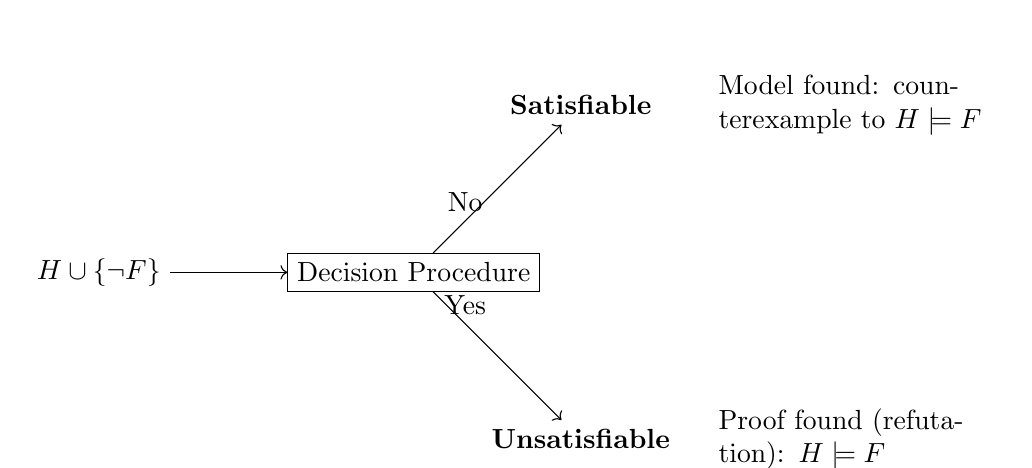
\begin{tikzpicture}[node distance=3cm, auto]
    \node (input) {$H \cup \{\neg F\}$};
    \node (procedure) [rectangle, draw, right of=input, node distance=4cm] {Decision Procedure};
    \node (unsat) [below right of=procedure, node distance=3cm] {\textbf{Unsatisfiable}};
    \node (sat) [above right of=procedure, node distance=3cm] {\textbf{Satisfiable}};
    
    \draw[->] (input) -- (procedure);
    \draw[->] (procedure) -- node[near start, above] {Yes} (unsat);
    \draw[->] (procedure) -- node[near start, above] {No} (sat);
    
    \node[right of=unsat, node distance=3.5cm, text width=3.5cm] {Proof found (refutation): $H \models F$};
    \node[right of=sat, node distance=3.5cm, text width=3.5cm] {Model found: counterexample to $H \models F$};
\end{tikzpicture}
\end{center}

\textbf{Two possible outcomes}:
\begin{itemize}
    \item \textbf{Unsatisfiable}: The procedure derives a contradiction, producing a \textbf{refutation} (proof) that $H \models F$
    \item \textbf{Satisfiable}: The procedure finds a model $\mathcal{I}$ of $H \cup \{\neg F\}$, which serves as a \textbf{counterexample} showing that $H \not\models F$
\end{itemize}

This refutational approach forms the foundation of modern automated theorem provers and SAT solvers, reducing the problem of proving logical consequence to the problem of detecting unsatisfiability.




\newpage

\part{Free Variables and Satisfiability}

\section{Satisfiability of Formulas with Free Variables}

\subsection{The Problem of Free Variables}

In our previous definition of satisfiability, we considered the semantics of logical connectives and quantifiers, but we did not fully address the treatment of \textbf{free variables}. Recall that a variable can be either:
\begin{itemize}
    \item \textbf{Bound}: The variable falls within the scope of a quantifier
    \item \textbf{Free}: The variable does not fall within the scope of any quantifier
\end{itemize}

The presence of free variables requires careful consideration when determining satisfiability, as their interpretation depends on the variable assignment $\beta$.

\subsection{Motivating Example}

Consider the following formula:
\[
F: \forall x \, (f(x, x) = x \wedge R(x, y))
\]

This formula contains:
\begin{itemize}
    \item A bound variable $x$ (quantified by $\forall$)
    \item A free variable $y$ (not quantified)
\end{itemize}

\subsection{Semantic Evaluation with Free Variables}

To determine whether an interpretation $\mathcal{I} = \langle D, \Phi \rangle$ with assignment $\beta$ satisfies $F$, we write $\mathcal{I} \models_\beta F$ and proceed as follows:

By the semantics of universal quantification, we need to check that for all $d \in D$:
\[
\mathcal{I} \models_{\beta[x \leftarrow d]} (f(x, x) = x \wedge R(x, y))
\]

This requires verifying both conjuncts under the updated assignment $\beta[x \leftarrow d]$:

\textbf{First conjunct}: $\mathcal{I} \models_{\beta[x \leftarrow d]} f(x, x) = x$

This holds if and only if:
\[
(\Phi(f)(d, d), d) \in \Phi(=)
\]
where $\Phi(=)$ represents the identity relation. In other words, we require that $\Phi(f)(d, d) = d$ for all $d \in D$.

\textbf{Second conjunct}: $\mathcal{I} \models_{\beta[x \leftarrow d]} R(x, y)$

This holds if and only if:
\[
(d, \beta(y)) \in \Phi(R)
\]

Let $\beta(y) = d'$ for some $d' \in D$. Then we require $(d, d') \in \Phi(R)$ for all $d \in D$.

\subsection{Existential Closure}

The key observation is that the satisfiability of a formula with free variables is intimately connected to its \textbf{existential closure}.

\begin{tcolorbox}[colback=green!5!white,colframe=green!75!black,title=\textbf{Existential Closure}]
\begin{definition}[Existential Closure]
The existential closure of a formula $F$, denoted $\exists^* F$, is obtained by adding an existential quantifier for every free variable in $F$.
\end{definition}
\end{tcolorbox}

For example, if $F$ contains free variables $y_1, y_2, \dots, y_n$, then:
\[
\exists^* F = \exists y_1 \, \exists y_2 \, \cdots \, \exists y_n \, F
\]

Returning to our example, if we consider the existential closure by quantifying the free variable $y$:
\[
\exists y \, \forall x \, (f(x, x) = x \wedge R(x, y))
\]

Under this interpretation, we need to verify that there exists some $d' \in D$ such that for all $d \in D$:
\[
\mathcal{I} \models_{\beta[x \leftarrow d, y \leftarrow d']} R(x, y)
\]
which means $(d, d') \in \Phi(R)$ for all $d \in D$.

\subsection{Satisfiability for Open Formulas}

We now provide the complete definition of satisfiability that handles both closed and open formulas.

\begin{tcolorbox}[colback=blue!5!white,colframe=blue!75!black,title=\textbf{Satisfiability - Complete Definition}]
\begin{definition}[Satisfiability - Complete Definition]
A formula $F$ is \textbf{satisfiable} if:
\begin{itemize}
    \item \textbf{Case 1 (Closed formula)}: If $F$ is a sentence (contains no free variables), then $F$ is satisfiable if there exists an interpretation $\mathcal{I}$ such that $\mathcal{I} \models F$.
    
    \item \textbf{Case 2 (Open formula)}: If $F$ contains free variables, then $F$ is satisfiable if there exists an interpretation $\mathcal{I}$ and a variable assignment $\beta$ such that $\mathcal{I} \models_\beta F$.
\end{itemize}
\end{definition}
\end{tcolorbox}

\begin{theorem}[Satisfiability and Existential Closure]
A formula $F$ with free variables is satisfiable if and only if its existential closure $\exists^* F$ is satisfiable.
\end{theorem}

\begin{proof}
Let $F$ be a formula with free variables $y_1, \dots, y_n$, and let $\exists^* F = \exists y_1 \, \cdots \, \exists y_n \, F$.

\textbf{($\Rightarrow$)} Suppose $F$ is satisfiable. Then there exists an interpretation $\mathcal{I}$ and assignment $\beta$ such that $\mathcal{I} \models_\beta F$. Let $d_i = \beta(y_i)$ for $i = 1, \dots, n$. Then by the semantics of existential quantification applied repeatedly, $\mathcal{I} \models \exists^* F$.

\textbf{($\Leftarrow$)} Suppose $\exists^* F$ is satisfiable. Then there exists an interpretation $\mathcal{I}$ such that $\mathcal{I} \models \exists y_1 \, \cdots \, \exists y_n \, F$. By the semantics of existential quantification, there exist $d_1, \dots, d_n \in D$ such that $\mathcal{I} \models_{\beta[y_1 \leftarrow d_1, \dots, y_n \leftarrow d_n]} F$. Therefore, $F$ is satisfiable.
\end{proof}

This result demonstrates that when checking satisfiability of formulas with free variables, we can equivalently check the satisfiability of their existential closures, treating free variables as existentially quantified.

\subsection{Universal Closure and Validity}

Dually, we can consider the \textbf{universal closure} of a formula with free variables.

\begin{theorem}[Validity and Universal Closure]
A formula $F$ with free variables is valid if and only if its universal closure $\forall^* F$ is valid.
\end{theorem}

The intuition is straightforward: if $F$ contains free variables, then $F$ is valid if for all interpretations $\mathcal{I}$ and for all assignments $\beta$, we have $\mathcal{I} \models_\beta F$. This is precisely the condition for the universal closure $\forall^* F$ to be valid.

\newpage

\section{Decidability and Semidecidability in First-Order Logic}

\subsection{Computational Complexity of First-Order Logic}

While certain restricted fragments of first-order logic admit decision procedures, the general case presents fundamental computational limitations:

\begin{tcolorbox}[colback=red!5!white,colframe=red!75!black,title=\textbf{Decidability in First-Order Logic}]
\begin{itemize}
    \item \textbf{Unsatisfiability} in first-order logic is \textbf{semidecidable} (recursively enumerable)
    \item \textbf{Satisfiability} in first-order logic is \textbf{not even semidecidable}
\end{itemize}
\end{tcolorbox}

\begin{remark}
Recall that if a decision problem $A$ is semidecidable and its complement $\neg A$ is also semidecidable, then $A$ is decidable. The decision procedure can be obtained by running both semidecision procedures in parallel: if the instance belongs to $A$, the first procedure will eventually terminate with "yes"; if the instance belongs to $\neg A$, the second procedure will eventually terminate with "yes".
\end{remark}

\subsection{Review: Semi-Decision Procedures}

Consider the problem of determining whether $H \models F$ (logical consequence).

\textbf{Semi-decision procedure for unsatisfiability}:
\begin{center}
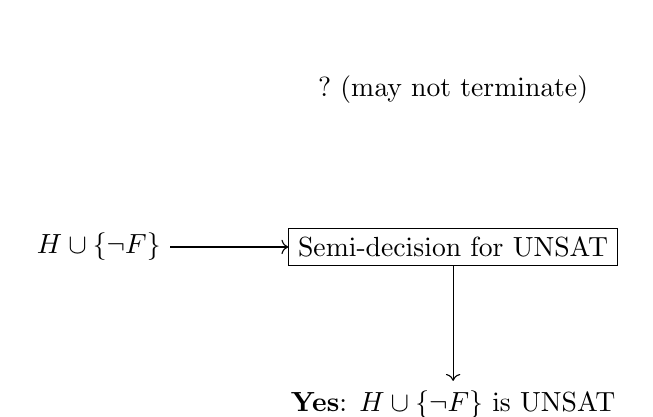
\begin{tikzpicture}[node distance=3cm, auto]
    \node (input) {$H \cup \{\neg F\}$};
    \node (procedure) [rectangle, draw, right of=input, node distance=4.5cm] {Semi-decision for UNSAT};
    \node (yes) [below of=procedure, node distance=2cm] {\textbf{Yes}: $H \cup \{\neg F\}$ is UNSAT};
    \node (unknown) [above of=procedure, node distance=2cm] {$?$ (may not terminate)};
    
    \draw[->] (input) -- (procedure);
    \draw[->] (procedure) -- (yes);
\end{tikzpicture}
\end{center}

If the procedure terminates with "yes", we have proven $H \models F$ by refutation. However, if $H \cup \{\neg F\}$ is satisfiable, the procedure may run indefinitely.

\textbf{Semi-decision procedure for satisfiability}:
\begin{center}
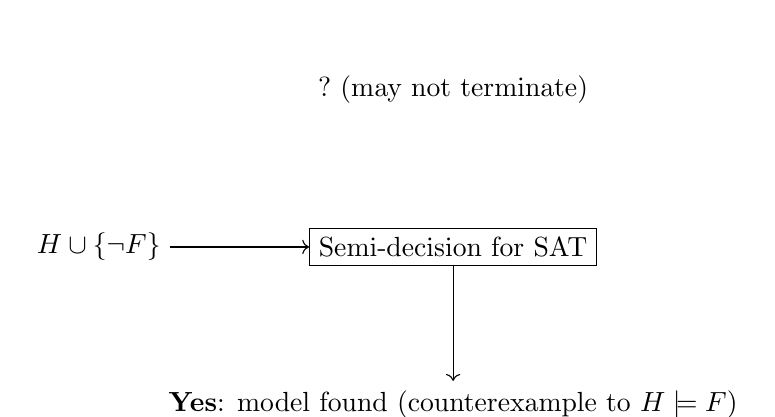
\begin{tikzpicture}[node distance=3cm, auto]
    \node (input) {$H \cup \{\neg F\}$};
    \node (procedure) [rectangle, draw, right of=input, node distance=4.5cm] {Semi-decision for SAT};
    \node (yes) [below of=procedure, node distance=2cm] {\textbf{Yes}: model found (counterexample to $H \models F$)};
    \node (unknown) [above of=procedure, node distance=2cm] {$?$ (may not terminate)};
    
    \draw[->] (input) -- (procedure);
    \draw[->] (procedure) -- (yes);
\end{tikzpicture}
\end{center}

If this procedure terminates with "yes", we have found a countermodel showing $H \not\models F$. However, such a procedure does not exist for general first-order logic.

\subsection{The Need for Restricted Theories}

To obtain decision procedures, we must restrict our attention to \textbf{decidable fragments} of first-order logic. This motivates the study of \textbf{first-order theories}---logical systems with additional structure that enable algorithmic reasoning.

\section{First-Order Theories}

\subsection{Definition of a First-Order Theory}

\begin{tcolorbox}[colback=purple!5!white,colframe=purple!75!black,title=\textbf{First-Order Theory}]
\begin{definition}[First-Order Theory]
A \textbf{first-order theory} is a pair $\mathcal{T} = \langle \Sigma, \mathcal{A} \rangle$ where:
\begin{itemize}
    \item $\Sigma$ is a \textbf{signature} (defining the vocabulary of the theory)
    \item $\mathcal{A}$ is a set of \textbf{axioms}---closed formulas (sentences) that we assume to hold in all models of the theory
\end{itemize}
\end{definition}
\end{tcolorbox}

The axioms define properties of specific symbols in the signature, giving them fixed interpretations across all models of the theory.

\subsection{The Theory of Equality}

A fundamental example is the \textbf{theory of equality} $\mathcal{T}_E = \langle \Sigma_E, \mathcal{A}_E \rangle$.

\textbf{Signature}: The signature of the theory of equality is:
\[
\Sigma_E = \{=\} \cup C \cup \mathcal{F} \cup \mathcal{P}
\]
where:
\begin{itemize}
    \item $=$ is the equality predicate (interpreted symbol)
    \item $C$ is a set of constant symbols (uninterpreted)
    \item $\mathcal{F}$ is a set of function symbols (uninterpreted)
    \item $\mathcal{P}$ is a set of predicate symbols (uninterpreted)
\end{itemize}

\textbf{Example signature}: Consider $\Sigma = \{a, b, f, Q, =\}$. The symbols $a, b, f, Q$ are \textbf{free} (uninterpreted), whereas $=$ (equality) is \textbf{defined} by the axioms of the theory.

\subsection{Axioms of Equality}

The axiom set $\mathcal{A}_E$ consists of formulas that characterize equality as a congruence relation.

\textbf{Equivalence relation axioms}:
\begin{align*}
&\forall x \, (x = x) && \text{(Reflexivity)} \\
&\forall x \, \forall y \, (x = y \rightarrow y = x) && \text{(Symmetry)} \\
&\forall x \, \forall y \, \forall z \, ((x = y \wedge y = z) \rightarrow x = z) && \text{(Transitivity)}
\end{align*}

These three axioms establish that equality is an equivalence relation.

\textbf{Congruence axioms for function symbols}: For each function symbol $f \in \mathcal{F}$ of arity $n$:
\[
\forall \vec{x} \, \forall \vec{y} \, \left( \bigwedge_{i=1}^{n} x_i = y_i \right) \rightarrow f(x_1, \dots, x_n) = f(y_1, \dots, y_n)
\]
where $\vec{x} = (x_1, \dots, x_n)$ and $\vec{y} = (y_1, \dots, y_n)$.

This axiom states that $f$ respects equality: equal inputs produce equal outputs.

\textbf{Congruence axioms for predicate symbols}: For each predicate symbol $R \in \mathcal{P}$ of arity $n$:
\[
\forall \vec{x} \, \forall \vec{y} \, \left( \bigwedge_{i=1}^{n} x_i = y_i \right) \rightarrow (R(x_1, \dots, x_n) \leftrightarrow R(y_1, \dots, y_n))
\]

This axiom states that $R$ respects equality: the truth value of $R$ depends only on the equivalence classes of its arguments.

\subsection{Models of a Theory}

\begin{definition}[$\mathcal{T}$-Model]
A \textbf{$\mathcal{T}$-model} is an interpretation $\mathcal{I}$ such that $\mathcal{I} \models \mathcal{A}$ (i.e., $\mathcal{I}$ satisfies all axioms in $\mathcal{A}$).
\end{definition}

\subsection{Satisfiability and Validity Relative to a Theory}

\begin{definition}[$\mathcal{T}$-Satisfiability]
A formula $G$ is \textbf{$\mathcal{T}$-satisfiable} if there exists a $\mathcal{T}$-model $\mathcal{I}$ such that $\mathcal{I} \models G$.
\end{definition}

\begin{definition}[$\mathcal{T}$-Validity]
A formula $G$ is \textbf{$\mathcal{T}$-valid} if for all $\mathcal{T}$-models $\mathcal{I}$, we have $\mathcal{I} \models G$.

Equivalently, $G$ is a logical consequence of the axioms: $\mathcal{A} \models G$.
\end{definition}

\subsection{Example: Satisfiability vs. $\mathcal{T}_E$-Satisfiability}

Consider the set of formulas:
\[
S = \{ P(a), \neg P(b), a = b \}
\]

\textbf{Claim}: $S$ is satisfiable in general first-order logic, but $S$ is \textbf{not $\mathcal{T}_E$-satisfiable}.

\begin{proof}
\textbf{Satisfiability}: We can construct an interpretation $\mathcal{I}$ with domain $D = \{d_1, d_2\}$ where:
\begin{itemize}
    \item $\Phi(a) = d_1$, $\Phi(b) = d_2$
    \item $\Phi(P) = \{d_1\}$
    \item $\Phi(=) = \{(d_1, d_1), (d_2, d_2), (d_1, d_2), (d_2, d_1)\}$ (universal relation)
\end{itemize}
Then $\mathcal{I} \models P(a)$, $\mathcal{I} \models \neg P(b)$, and $\mathcal{I} \models a = b$, so $\mathcal{I} \models S$.

\textbf{$\mathcal{T}_E$-Unsatisfiability}: In any $\mathcal{T}_E$-model, equality must satisfy the congruence axioms. If $\mathcal{I} \models a = b$ and $\mathcal{I} \models P(a)$, then by the congruence axiom for $P$, we must have $\mathcal{I} \models P(b)$, contradicting $\mathcal{I} \models \neg P(b)$. Therefore, no $\mathcal{T}_E$-model satisfies $S$.
\end{proof}

This example illustrates that satisfiability relative to a theory is more restrictive than general satisfiability, as models must respect the additional constraints imposed by the theory's axioms.

\section{Quantifier-Free Fragments and Decidability}

\subsection{The Quantifier-Free Fragment of $\mathcal{T}_E$}

While the full theory of equality $\mathcal{T}_E$ is undecidable, its \textbf{quantifier-free fragment} admits a decision procedure.

\begin{definition}[Quantifier-Free Fragment]
The \textbf{quantifier-free fragment} of first-order logic consists of all formulas that do not contain quantifiers ($\forall$ or $\exists$).

For a theory $\mathcal{T}$, the quantifier-free fragment allows quantifiers to appear only in the axioms, not in the input formulas to be checked for satisfiability.
\end{definition}

Our goal is to develop a decision procedure for the quantifier-free fragment of $\mathcal{T}_E$. We will focus initially on deciding satisfiability for sets (or conjunctions) of literals, and then extend this to arbitrary quantifier-free formulas using normal forms.

\subsection{Normal Forms}

To handle arbitrary quantifier-free formulas, we introduce two important normal forms that facilitate systematic reasoning.

\subsubsection{Negation Normal Form (NNF)}

\begin{tcolorbox}[colback=cyan!5!white,colframe=cyan!75!black,title=\textbf{Negation Normal Form (NNF)}]
\begin{definition}[Negation Normal Form]
A formula is in \textbf{Negation Normal Form (NNF)} if:
\begin{itemize}
    \item The only logical connectives are $\wedge$, $\vee$, and $\neg$
    \item Negation ($\neg$) applies only to atomic formulas (atoms)
\end{itemize}
\end{definition}
\end{tcolorbox}

Any quantifier-free formula can be converted to NNF by applying the following equivalence-preserving transformations:

\begin{align*}
H \leftrightarrow G &\equiv (H \rightarrow G) \wedge (G \rightarrow H) && \text{(Eliminate biconditional)} \\
H \rightarrow G &\equiv \neg H \vee G && \text{(Eliminate implication)} \\
\neg (H \wedge G) &\equiv \neg H \vee \neg G && \text{(De Morgan's law)} \\
\neg (H \vee G) &\equiv \neg H \wedge \neg G && \text{(De Morgan's law)} \\
\neg \neg H &\equiv H && \text{(Double negation elimination)}
\end{align*}

\subsubsection{Disjunctive Normal Form (DNF)}

\begin{tcolorbox}[colback=cyan!5!white,colframe=cyan!75!black,title=\textbf{Disjunctive Normal Form (DNF)}]
\begin{definition}[Disjunctive Normal Form]
A formula is in \textbf{Disjunctive Normal Form (DNF)} if it is a disjunction of conjunctions of literals:
\[
\bigvee_{i=1}^{k} \left( \bigwedge_{j=1}^{n_i} L_{i,j} \right)
\]
where each $L_{i,j}$ is a literal (an atomic formula or its negation).
\end{definition}
\end{tcolorbox}

Equivalently, a DNF formula has the structure:
\[
(L_{1,1} \wedge L_{1,2} \wedge \cdots \wedge L_{1,n_1}) \vee (L_{2,1} \wedge L_{2,2} \wedge \cdots \wedge L_{2,n_2}) \vee \cdots \vee (L_{k,1} \wedge L_{k,2} \wedge \cdots \wedge L_{k,n_k})
\]

\subsection{Conversion to DNF}

Any quantifier-free formula $F$ can be systematically converted to an equivalent DNF formula through a two-stage process:

\begin{center}
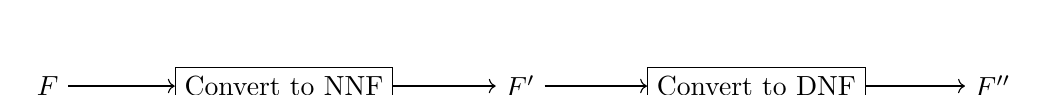
\begin{tikzpicture}[node distance=3cm, auto]
    \node (F) {$F$};
    \node (NNF) [rectangle, draw, right of=F, node distance=3cm] {Convert to NNF};
    \node (Fprime) [right of=NNF, node distance=3cm] {$F'$};
    \node (DNF) [rectangle, draw, right of=Fprime, node distance=3cm] {Convert to DNF};
    \node (Fdoubleprime) [right of=DNF, node distance=3cm] {$F''$};
    
    \draw[->] (F) -- (NNF);
    \draw[->] (NNF) -- (Fprime);
    \draw[->] (Fprime) -- (DNF);
    \draw[->] (DNF) -- (Fdoubleprime);
\end{tikzpicture}
\end{center}

\textbf{Stage 1}: Convert $F$ to NNF using the transformations above, obtaining $F'$.

\textbf{Stage 2}: Convert $F'$ to DNF by repeatedly applying the distributivity law:
\[
H \wedge (G_1 \vee G_2) \equiv (H \wedge G_1) \vee (H \wedge G_2)
\]

This transformation pushes conjunctions inward and disjunctions outward, resulting in a disjunction of conjunctions.

\subsection{Decision Procedure for Quantifier-Free $\mathcal{T}_E$}

The decision procedure operates on conjunctions of literals. Given a set (or conjunction) $S$ of literals:

\begin{center}
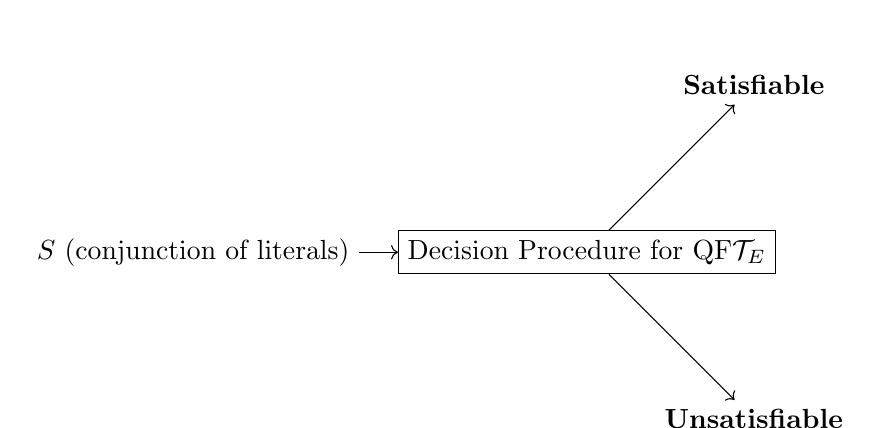
\begin{tikzpicture}[node distance=3cm, auto]
    \node (input) {$S$ (conjunction of literals)};
    \node (procedure) [rectangle, draw, right of=input, node distance=5cm] {Decision Procedure for $\text{QF}\mathcal{T}_E$};
    \node (unsat) [below right of=procedure, node distance=3cm] {\textbf{Unsatisfiable}};
    \node (sat) [above right of=procedure, node distance=3cm] {\textbf{Satisfiable}};
    
    \draw[->] (input) -- (procedure);
    \draw[->] (procedure) -- node[near start, above] {} (sat);
    \draw[->] (procedure) -- node[near start, below] {} (unsat);
\end{tikzpicture}
\end{center}

\textbf{Extension to arbitrary quantifier-free formulas}: For a general quantifier-free formula $F$:
\begin{enumerate}
    \item Convert $F$ to NNF, obtaining $F'$
    \item Convert $F'$ to DNF, obtaining $F'' = \bigvee_{i=1}^{k} C_i$ where each $C_i$ is a conjunction of literals
    \item Apply the decision procedure to each conjunction $C_i$
    \item $F$ is satisfiable if and only if at least one $C_i$ is satisfiable
\end{enumerate}

This reduction allows us to decide satisfiability for arbitrary quantifier-free formulas by deciding satisfiability for each disjunct independently.

\subsection{Elimination of Non-Equality Predicates}

The decision procedure for quantifier-free $\mathcal{T}_E$ assumes that the only predicate symbol in the formula is equality ($=$). However, formulas may contain additional predicate symbols. We now show how to eliminate such predicates through a satisfiability-preserving transformation.

\subsubsection{The Transformation}

\begin{tcolorbox}[colback=yellow!10!white,colframe=yellow!75!black,title=\textbf{Predicate Elimination}]
\begin{definition}[Predicate Elimination]
Given an occurrence of a predicate symbol $P$ of arity $n$ applied to terms $t_1, \dots, t_n$, we eliminate $P$ by introducing:
\begin{itemize}
    \item A fresh function symbol $f_P$ (one for each predicate symbol $P \neq {=}$)
    \item A fresh constant symbol $\bullet$ (the same constant for all predicates)
\end{itemize}

The transformation replaces predicate applications with equality constraints:
\begin{align*}
P(t_1, \dots, t_n) &\mapsto f_P(t_1, \dots, t_n) = \bullet \\
\neg P(t_1, \dots, t_n) &\mapsto f_P(t_1, \dots, t_n) \neq \bullet
\end{align*}
\end{definition}
\end{tcolorbox}

\textbf{Intuition}: The predicate $P(t_1, \dots, t_n)$ is true if and only if the term $f_P(t_1, \dots, t_n)$ evaluates to the distinguished constant $\bullet$.

\subsubsection{Satisfiability Preservation}

\begin{theorem}[Satisfiability Preservation]
Let $F$ be a quantifier-free formula and let $F'$ be the result of applying predicate elimination to $F$. Then $F$ is satisfiable if and only if $F'$ is satisfiable in models with cardinality greater than 1.
\end{theorem}

\begin{remark}
The restriction to models with cardinality greater than 1 is necessary to avoid trivial models. In a model with domain $D = \{d\}$ (cardinality 1), all terms evaluate to the same element $d$, making all equalities trivially true and potentially invalidating the transformation.
\end{remark}

\subsubsection{Example: The Need for Cardinality Restriction}

Consider the following two formulas:

\textbf{Original formula}:
\[
S_1 = \{\forall x \, \forall y \, (x = y), \neg P(a)\}
\]

This formula is $\mathcal{T}_E$-satisfiable. We can construct a model with domain $D = \{d_1, d_2\}$ where:
\begin{itemize}
    \item $\Phi(a) = d_1$
    \item $\Phi(P) = \{d_2\}$ (so $d_1 \notin \Phi(P)$, making $\neg P(a)$ true)
    \item The first axiom $\forall x \, \forall y \, (x = y)$ is vacuously false in this model, but if we interpret it as requiring equality to be universal, we need a different construction
\end{itemize}

Actually, let's reconsider: $\{\forall x \, \forall y \, (x = y), \neg P(a)\}$ asserts that all elements are equal (domain has cardinality 1) and $P(a)$ is false. This is satisfiable in a model with $D = \{d\}$, $\Phi(a) = d$, and $\Phi(P) = \emptyset$.

\textbf{Transformed formula}:
\[
S_2 = \{\forall x \, \forall y \, (x = y), f_P(a) \neq \bullet\}
\]

In a model with cardinality 1, we have $D = \{d\}$, so $\Phi(f_P)(d) = d$ and $\Phi(\bullet) = d$. Therefore, $f_P(a) = \bullet$, contradicting $f_P(a) \neq \bullet$. Thus $S_2$ is unsatisfiable in models of cardinality 1.

This example demonstrates that the transformation preserves satisfiability only when we exclude trivial models with cardinality 1.

\subsection{Treatment of Free Variables}

In quantifier-free formulas, free variables may appear. For the purposes of satisfiability checking, free variables are treated analogously to constants.

\begin{remark}[Free Variables as Constants]
To determine satisfiability of a formula $F$ with free variables $x_1, \dots, x_k$, we need to find an interpretation $\mathcal{I}$ and an assignment $\beta$ such that $\mathcal{I} \models_\beta F$.

Equivalently, we can treat each free variable $x_i$ as a fresh constant symbol $c_i$ and check satisfiability of the resulting closed formula. The formula is satisfiable if and only if there exist domain elements that can be assigned to these constants to satisfy the formula.
\end{remark}

This observation allows us to reduce the satisfiability problem for formulas with free variables to the satisfiability problem for closed formulas by a simple syntactic substitution.

\section{The Congruence Closure Algorithm}

\subsection{Motivating Example}

Consider the following conjunction of literals:
\[
x = g(x) \wedge f(x, g(g(x))) \neq g(x) \wedge f(x, x) = g(g(x))
\]

\textbf{Question}: Is this formula satisfiable or unsatisfiable?

\textbf{Intuitive analysis}: This formula appears to be unsatisfiable. From $x = g(x)$, we can derive $g(x) = g(g(x))$ by applying the function $g$ to both sides (congruence). Then from $f(x, x) = g(g(x))$ and the derived equality $g(x) = g(g(x))$, we obtain $f(x, x) = g(x)$. But we also have $x = g(x)$, so by congruence on $f$, we get $f(x, x) = f(x, g(x))$. However, we need to check whether $f(x, g(g(x))) = g(x)$ follows from the positive equalities, which would contradict $f(x, g(g(x))) \neq g(x)$.

\subsection{The Congruence Closure Decision Procedure}

\begin{tcolorbox}[colback=orange!10!white,colframe=orange!75!black,title=\textbf{Congruence Closure Algorithm}]
The \textbf{congruence closure algorithm} is a decision procedure for satisfiability in the quantifier-free fragment of the theory of equality. The algorithm operates as follows:

\begin{enumerate}
    \item \textbf{Build the smallest congruence}: Construct the smallest congruence relation that satisfies all positive equalities in the input formula
    \item \textbf{Check negative equalities}: For each negative equality $s \neq t$ in the input, check whether $s$ and $t$ belong to the same equivalence class in the congruence
    \item \textbf{Determine satisfiability}:
    \begin{itemize}
        \item If any pair $(s, t)$ with $s \neq t$ belongs to the same equivalence class, the formula is \textbf{unsatisfiable}
        \item Otherwise, the congruence provides a model, and the formula is \textbf{satisfiable}
    \end{itemize}
\end{enumerate}
\end{tcolorbox}

The key insight is that the smallest congruence containing all positive equalities is included in every congruence that satisfies those equalities. Therefore, if a negative equality is violated in the smallest congruence, it must be violated in every model.

\subsection{Equivalence Relations and Partitions}

Before describing the algorithm in detail, we recall fundamental properties of equivalence relations.

\begin{tcolorbox}[colback=teal!10!white,colframe=teal!75!black,title=\textbf{Equivalence Relation}]
\begin{definition}[Equivalence Relation]
An \textbf{equivalence relation} $R$ on a set $S$ is a binary relation that is:
\begin{itemize}
    \item \textbf{Reflexive}: $\forall s \in S, \, s \, R \, s$
    \item \textbf{Symmetric}: $\forall s, t \in S, \, s \, R \, t \implies t \, R \, s$
    \item \textbf{Transitive}: $\forall s, t, u \in S, \, (s \, R \, t \wedge t \, R \, u) \implies s \, R \, u$
\end{itemize}
\end{definition}
\end{tcolorbox}

\begin{definition}[Equivalence Class]
Given an equivalence relation $R$ on set $S$, the \textbf{equivalence class} of an element $s \in S$ is:
\[
[s]_R = \{s' \in S \mid s' \, R \, s\}
\]
\end{definition}

\begin{definition}[Quotient Set]
The \textbf{quotient set} $S/R$ is the set of all equivalence classes:
\[
S/R = \{[s]_R \mid s \in S\}
\]
\end{definition}

\begin{proposition}[Partition Property]
An equivalence relation $R$ on $S$ induces a partition of $S$. That is, for any two distinct equivalence classes $[s]_R$ and $[p]_R$:
\[
s \not\sim_R p \quad \implies \quad [s]_R \cap [p]_R = \emptyset
\]
where $s \sim_R p$ denotes $s \, R \, p$.

Conversely, every element belongs to exactly one equivalence class, and the union of all equivalence classes equals $S$.
\end{proposition}

This partition property is fundamental to the congruence closure algorithm, as it allows us to represent the congruence relation efficiently using a union-find data structure.

\newpage

\part{Decision Procedures for Quantifier-Free Theories}

\section{The Congruence Closure Algorithm}

\subsection{Computing Congruence Closure}

We now describe how to compute the congruence closure for the quantifier-free fragment of the theory of equality $\mathcal{T}_E$.

\subsubsection{Input Problem Structure}

Consider an input formula $F$ consisting of a conjunction of equality and disequality literals:
\[
F = \underbrace{\{s_1 = t_1, \dots, s_n = t_n\}}_{F^+} \cup \underbrace{\{s_{n+1} \neq t_{n+1}, \dots, s_{n+m} \neq t_{n+m}\}}_{F^-}
\]

where:
\begin{itemize}
    \item $F^+$ denotes the set of \textbf{positive equalities} (equations)
    \item $F^-$ denotes the set of \textbf{negative equalities} (disequations)
\end{itemize}

The congruence closure algorithm will construct the smallest congruence containing all equalities in $F^+$, then check whether any disequality in $F^-$ is violated.

\subsubsection{Equivalence Relations and Representatives}

Given a binary equivalence relation $R \subseteq S \times S$ on a set $S$, we can construct its quotient:
\[
S/R = \{[s]_R \mid s \in S\}
\]

where the equivalence class of $s$ is:
\[
[s]_R = \{p \in S \mid p \, R \, s\}
\]

The element $s$ is called a \textbf{representative} of the equivalence class $[s]_R$.

\subsubsection{Disjointness of Equivalence Classes}

\begin{proposition}[Disjoint Classes]
For any two equivalence classes $[s_1]_R$ and $[s_2]_R$, either they are identical or they are disjoint:
\[
[s_1]_R \cap [s_2]_R \neq \emptyset \quad \implies \quad [s_1]_R = [s_2]_R
\]
\end{proposition}

\begin{proof}
Suppose there exists $p \in [s_1]_R \cap [s_2]_R$. Then:
\begin{itemize}
    \item $p \, R \, s_1$ (since $p \in [s_1]_R$)
    \item $p \, R \, s_2$ (since $p \in [s_2]_R$)
\end{itemize}

By symmetry and transitivity of $R$, we have $s_1 \, R \, s_2$. Therefore, for any $q \in [s_1]_R$, we have $q \, R \, s_1$ and $s_1 \, R \, s_2$, so by transitivity $q \, R \, s_2$, which means $q \in [s_2]_R$. Similarly, $[s_2]_R \subseteq [s_1]_R$. Thus $[s_1]_R = [s_2]_R$.
\end{proof}

\subsubsection{Example: Equivalence Closure}

Consider the binary relation:
\[
R = \{(a, b), (b, c), (d, d)\}
\]

We can visualize this as a directed graph:
\begin{center}
\begin{tikzpicture}[node distance=1.5cm, auto]
    \node (a) {$a$};
    \node (b) [right of=a] {$b$};
    \node (c) [right of=b] {$c$};
    \node (d) [right of=c, node distance=2.5cm] {$d$};
    
    \draw[->] (a) -- (b);
    \draw[->] (b) -- (c);
    \draw[->] (d) edge [loop right] (d);
\end{tikzpicture}
\end{center}

The \textbf{equivalence closure} $R^*$ of $R$ must include:
\begin{itemize}
    \item \textbf{Reflexivity}: $(a, a), (b, b), (c, c), (d, d)$
    \item \textbf{Symmetry}: $(b, a), (c, b)$
    \item \textbf{Transitivity}: $(a, c), (c, a)$
\end{itemize}

Thus:
\[
R^* = \{(a, a), (a, b), (a, c), (b, a), (b, b), (b, c), (c, a), (c, b), (c, c), (d, d)\}
\]

The quotient set is:
\[
S/R^* = \{\{a, b, c\}, \{d\}\}
\]

\begin{tcolorbox}[colback=green!5!white,colframe=green!75!black,title=\textbf{Equivalence Closure}]
\begin{definition}[Equivalence Closure]
Given a binary relation $R$ on set $S$, the \textbf{equivalence closure} of $R$, denoted $R^*$, is the $\subseteq$-smallest equivalence relation such that:
\begin{enumerate}
    \item $R^*$ is an equivalence relation
    \item $R \subseteq R^*$
\end{enumerate}

Equivalently, $R^*$ is the intersection of all equivalence relations containing $R$.
\end{definition}
\end{tcolorbox}

The equivalence closure can be computed by iteratively applying reflexivity, symmetry, and transitivity rules until a fixed point is reached.

\subsubsection{Understanding the $\subseteq$-Smallest Property}

\begin{proposition}[Minimality of Equivalence Closure]
Let $R$ be a binary relation and $R^*$ be its equivalence closure. For any equivalence relation $P$ such that $R \subseteq P$, we have $R^* \subseteq P$.
\end{proposition}

This means that $R^*$ is the \textbf{smallest} equivalence relation containing $R$ with respect to the subset ordering $\subseteq$.

\begin{tcolorbox}[colback=green!5!white,colframe=green!75!black,title=\textbf{Congruence Closure}]
\begin{definition}[Congruence Closure]
Given a binary relation $R$, the \textbf{congruence closure} of $R$, denoted $R^*_{\text{cong}}$, is the $\subseteq$-smallest relation such that:
\begin{enumerate}
    \item $R^*_{\text{cong}}$ is a congruence relation
    \item $R \subseteq R^*_{\text{cong}}$
\end{enumerate}
\end{definition}
\end{tcolorbox}

A congruence relation is an equivalence relation that is preserved under function application: if $s_1 \sim t_1, \dots, s_n \sim t_n$, then $f(s_1, \dots, s_n) \sim f(t_1, \dots, t_n)$ for all function symbols $f$.

\subsubsection{Example: Refinement of Equivalence Relations}

To illustrate the concept of one equivalence relation being smaller (finer) than another, consider the following example on the natural numbers $\N$.

\textbf{Equivalence modulo 2}: Define the relation $\equiv_2 \subseteq \N \times \N$ by:
\[
n \equiv_2 m \quad \text{iff} \quad n \equiv m \pmod{2}
\]

This relation partitions $\N$ into two equivalence classes:
\begin{center}
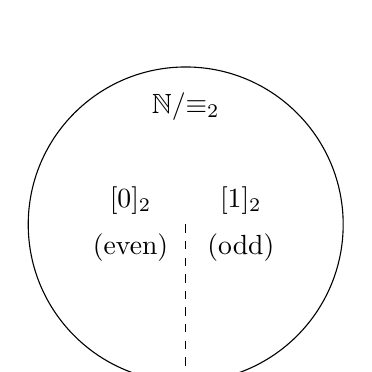
\begin{tikzpicture}
    \draw (0,0) circle (2cm);
    \node at (0, 1.5) {$\N/{\equiv_2}$};
    \draw[dashed] (0,0) -- (0,-2);
    \node at (-0.7, 0.3) {$[0]_2$};
    \node at (-0.7, -0.3) {(even)};
    \node at (0.7, 0.3) {$[1]_2$};
    \node at (0.7, -0.3) {(odd)};
\end{tikzpicture}
\end{center}

\textbf{Equivalence modulo 4}: Define the relation $\equiv_4 \subseteq \N \times \N$ by:
\[
n \equiv_4 m \quad \text{iff} \quad n \equiv m \pmod{4}
\]

This relation partitions $\N$ into four equivalence classes:
\begin{center}
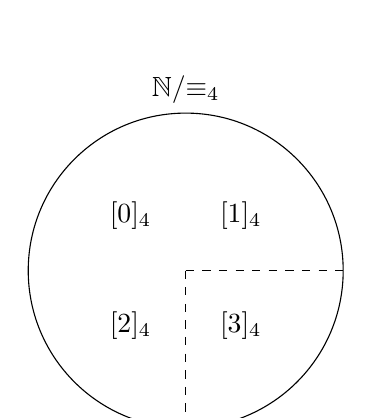
\begin{tikzpicture}
    \draw (0,0) circle (2cm);
    \node at (0, 2.3) {$\N/{\equiv_4}$};
    \draw[dashed] (0,0) -- (0,-2);
    \draw[dashed] (0,0) -- (2,0);
    \node at (-0.7, 0.7) {$[0]_4$};
    \node at (0.7, 0.7) {$[1]_4$};
    \node at (-0.7, -0.7) {$[2]_4$};
    \node at (0.7, -0.7) {$[3]_4$};
\end{tikzpicture}
\end{center}

\begin{proposition}[Refinement]
The relation $\equiv_4$ is a \textbf{refinement} of $\equiv_2$. That is:
\[
n \equiv_4 m \quad \implies \quad n \equiv_2 m
\]

However, the converse does not hold:
\[
n \equiv_2 m \quad \not\Rightarrow \quad n \equiv_4 m
\]
\end{proposition}

\begin{proof}
If $n \equiv_4 m$, then $n \equiv m \pmod{4}$, which means $n - m = 4k$ for some $k \in \mathbb{Z}$. Therefore, $n - m = 2(2k)$, so $n \equiv m \pmod{2}$, i.e., $n \equiv_2 m$.

For the converse, consider $n = 0$ and $m = 2$. Then $n \equiv_2 m$ (both are even), but $n \not\equiv_4 m$ (since $0 \equiv 0 \pmod{4}$ and $2 \equiv 2 \pmod{4}$).
\end{proof}

\textbf{Set-theoretic interpretation}: This means that $(n, m) \in {\equiv_4} \implies (n, m) \in {\equiv_2}$, so:
\[
{\equiv_4} \subseteq {\equiv_2}
\]

In this sense, $\equiv_4$ is \textbf{strictly smaller} than $\equiv_2$ (it is a proper subset), and provides a finer partition of $\N$.

\subsection{The Congruence Closure Decision Procedure}

We now return to the main problem: deciding satisfiability for a quantifier-free formula in the theory of equality.

\subsubsection{Algorithm Description}

Recall that the input formula $F$ has the form:
\[
F = \underbrace{\{s_1 = t_1, \dots, s_n = t_n\}}_{F^+} \cup \underbrace{\{s_{n+1} \neq t_{n+1}, \dots, s_{n+m} \neq t_{n+m}\}}_{F^-}
\]

The congruence closure algorithm proceeds as follows:

\begin{algorithm}[H]
\caption{Congruence Closure Decision Procedure}
\begin{algorithmic}[1]
\STATE \textbf{Input:} Formula $F = F^+ \cup F^-$
\STATE Compute the congruence closure $\text{CC}(F^+)$ of the positive equalities $F^+$
\STATE \textbf{for} $i = n+1$ to $n+m$ \textbf{do}
\STATE \quad \textbf{if} $(s_i, t_i) \in \text{CC}(F^+)$ \textbf{then}
\STATE \quad \quad \textbf{return} UNSATISFIABLE
\STATE \quad \textbf{end if}
\STATE \textbf{end for}
\STATE \textbf{return} SATISFIABLE
\end{algorithmic}
\end{algorithm}

\textbf{Step 1}: Compute $\text{CC}(F^+)$, the smallest congruence relation containing all pairs $(s_i, t_i)$ for $i = 1, \dots, n$.

\textbf{Step 2}: For each disequality $s_i \neq t_i$ in $F^-$ (where $n+1 \leq i \leq n+m$), check whether $(s_i, t_i)$ belongs to the same equivalence class in $\text{CC}(F^+)$.

\textbf{Step 3}: 
\begin{itemize}
    \item If $(s_j, t_j) \in \text{CC}(F^+)$ for some $j$ with $n+1 \leq j \leq n+m$, then $F$ is \textbf{unsatisfiable}
    \item Otherwise, $F$ is \textbf{satisfiable}
\end{itemize}

\begin{center}
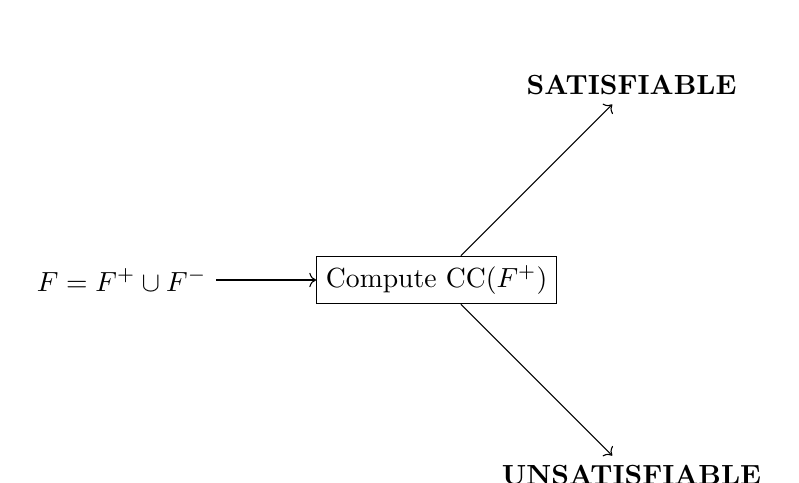
\begin{tikzpicture}[node distance=3cm, auto]
    \node (input) {$F = F^+ \cup F^-$};
    \node (cc) [rectangle, draw, right of=input, node distance=4cm] {Compute $\text{CC}(F^+)$};
    \node (unsat) [below right of=cc, node distance=3.5cm] {\textbf{UNSATISFIABLE}};
    \node (sat) [above right of=cc, node distance=3.5cm] {\textbf{SATISFIABLE}};
    
    \draw[->] (input) -- (cc);
    \draw[->] (cc) -- (unsat);
    \draw[->] (cc) -- (sat);
\end{tikzpicture}
\end{center}

\subsubsection{Correctness of the Algorithm}

\begin{theorem}[Soundness and Completeness]
The congruence closure algorithm is sound and complete for deciding satisfiability in the quantifier-free fragment of $\mathcal{T}_E$.
\end{theorem}

\begin{proof}[Proof sketch]
\textbf{Soundness (Unsatisfiability)}: Suppose there exists $j$ with $n+1 \leq j \leq n+m$ such that $(s_j, t_j) \in \text{CC}(F^+)$. 

Since $\text{CC}(F^+)$ is the smallest congruence relation containing $F^+$, the pair $(s_j, t_j)$ must belong to \emph{every} congruence relation that contains $F^+$. 

Therefore, in any model $\mathcal{I}$ that satisfies all equalities in $F^+$, we must have $\mathcal{I} \models s_j = t_j$. But $F$ also contains $s_j \neq t_j$, so $\mathcal{I} \not\models s_j \neq t_j$. Thus, no model can satisfy both $F^+$ and $F^-$, making $F$ unsatisfiable.

\textbf{Completeness (Satisfiability)}: If $(s_i, t_i) \notin \text{CC}(F^+)$ for all $i$ with $n+1 \leq i \leq n+m$, then we can construct a model by interpreting the equivalence classes of $\text{CC}(F^+)$ as domain elements. This model satisfies all equalities in $F^+$ (by construction) and all disequalities in $F^-$ (since the terms belong to different equivalence classes).
\end{proof}

The key insight is that the congruence closure captures exactly those equalities that are \emph{forced} by the positive equalities in $F^+$ together with the congruence axioms of equality.

\subsection{Examples: Manual Execution}

We now illustrate the congruence closure algorithm with concrete examples.

\subsubsection{Notation and Setup}

For a formula $F$ of the form:
\[
F = \{s_1 = t_1, \dots, s_n = t_n\} \cup \{s_{n+1} \neq t_{n+1}, \dots, s_{n+m} \neq t_{n+m}\}
\]

we define $S_F$ as the \textbf{set of all terms} that appear in $F$.

\subsubsection{Example 1}

Consider the formula:
\[
F = \{x = g(x), \, f(x, x) = g(g(x)), \, f(x, g(g(x))) \neq g(x)\}
\]

The set of terms is:
\[
S_F = \{x, \, g(x), \, f(x, x), \, g(g(x)), \, f(x, g(g(x)))\}
\]

\textbf{Notation}:
\begin{itemize}
    \item $x$ is a \textbf{free variable symbol}
    \item $f$ is a \textbf{binary function symbol} (arity 2)
    \item $g$ is a \textbf{unary function symbol} (arity 1)
\end{itemize}

\textbf{Positive equalities}: $F^+ = \{x = g(x), \, f(x, x) = g(g(x))\}$

\textbf{Negative equalities}: $F^- = \{f(x, g(g(x))) \neq g(x)\}$

\subsubsection{Example 2}

Consider the formula:
\[
F = \{f(a, b) = a, \, f(f(a, b), b) \neq a\}
\]

The set of terms is:
\[
S_F = \{f(a, b), \, a, \, b, \, f(f(a, b), b)\}
\]

\textbf{Notation}:
\begin{itemize}
    \item $a, b$ are \textbf{constant symbols} (by convention)
    \item $f$ is a \textbf{binary function symbol}
\end{itemize}

\textbf{Positive equalities}: $F^+ = \{f(a, b) = a\}$

\textbf{Negative equalities}: $F^- = \{f(f(a, b), b) \neq a\}$

\begin{remark}[Free Variables vs. Constants]
In the quantifier-free fragment, all variables are free. From a semantic perspective, free variables and constants can be used interchangeably: both are interpreted as arbitrary elements of the domain. The distinction is purely syntactic.
\end{remark}

\subsubsection{Step-by-Step Execution for Example 1}

We now execute the congruence closure algorithm on Example 1:
\[
F = \{x = g(x), \, f(x, x) = g(g(x)), \, f(x, g(g(x))) \neq g(x)\}
\]

\textbf{Step 1: Initialize the partition}

Create a partition of $S_F$ where every term is in its own singleton equivalence class:
\[
\{\{x\}, \{g(x)\}, \{f(x, x)\}, \{g(g(x))\}, \{f(x, g(g(x)))\}\}
\]

\textbf{Step 2: Process positive equalities}

For each equality $(s_i = t_i) \in F^+$ (for all $i$ with $1 \leq i \leq n$):
\begin{itemize}
    \item Unite the equivalence class of $s_i$ with the equivalence class of $t_i$
    \item Unite the classes of all terms in $S_F$ that become congruent as a consequence of $s_i = t_i$
\end{itemize}

\textbf{Processing $x = g(x)$}:

Merge the classes $\{x\}$ and $\{g(x)\}$:
\[
\{\{x, g(x)\}, \{f(x, x)\}, \{g(g(x))\}, \{f(x, g(g(x)))\}\}
\]

Since $x = g(x)$, by congruence we derive $g(x) = g(g(x))$ (applying $g$ to both sides). Merge these classes:
\[
\{\{x, g(x), g(g(x))\}, \{f(x, x)\}, \{f(x, g(g(x)))\}\}
\]

\textbf{Processing $f(x, x) = g(g(x))$}:

Since $g(g(x)) \in \{x, g(x), g(g(x))\}$ and $f(x, x) \in \{f(x, x)\}$, merge these classes:
\[
\{\{x, g(x), g(g(x)), f(x, x)\}, \{f(x, g(g(x)))\}\}
\]

Now check for congruence: since $x \sim g(g(x))$ (both in the same class), we have:
\[
f(x, x) \sim f(x, g(g(x)))
\]

by the congruence property (both arguments are in the same equivalence classes). Merge these classes:
\[
\{\{x, g(x), g(g(x)), f(x, x), f(x, g(g(x)))\}\}
\]

\textbf{Step 3: Check negative equalities}

Check whether $(s_i, t_i) \in \text{CC}(F^+)$ for all $i$ with $n+1 \leq i \leq n+m$.

For the disequality $f(x, g(g(x))) \neq g(x)$:
\begin{itemize}
    \item $f(x, g(g(x))) \in \{x, g(x), g(g(x)), f(x, x), f(x, g(g(x)))\}$
    \item $g(x) \in \{x, g(x), g(g(x)), f(x, x), f(x, g(g(x)))\}$
\end{itemize}

Both terms are in the same equivalence class, so $(f(x, g(g(x))), g(x)) \in \text{CC}(F^+)$.

\textbf{Conclusion}: The formula $F$ is \textbf{UNSATISFIABLE}.




\newpage

\section{Implementation of Congruence Closure on a DAG}

\subsection{DAG Representation}

The congruence closure algorithm can be implemented efficiently using a \textbf{Directed Acyclic Graph (DAG)} representation of the terms.

Consider the formula:
\[
F = \{x = g(x), \, f(x, x) = g(g(x))\} \cup \{f(x, g(g(x))) \neq g(x)\}
\]

The set of terms is:
\[
S_F = \{x, \, g(x), \, g(g(x)), \, f(x, x), \, f(x, g(g(x)))\}
\]

We represent these terms as a graph where:
\begin{itemize}
    \item Each term is a node
    \item Edges connect function symbols to their arguments
    \item We use $g$ and $g'$ to distinguish the two applications of function $g$
    \item We use $f$ and $f'$ to distinguish the two applications of function $f$
\end{itemize}

\begin{center}
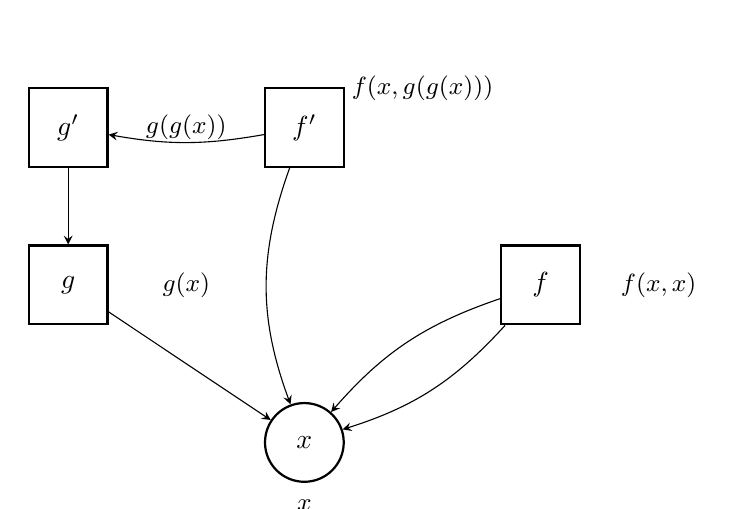
\begin{tikzpicture}[
    node/.style={circle, draw, minimum size=1cm, thick},
    func/.style={rectangle, draw, minimum size=1cm, thick},
    >=stealth,
    every edge/.style={draw, ->, thick}
]
    % Variable node (center)
    \node[node] (x) at (0, 0) {$x$};
    
    % First g application: g(x)
    \node[func] (g) at (-3, 2) {$g$};
    \draw[->] (g) -- (x);
    
    % Second g application: g(g(x))
    \node[func] (g2) at (-3, 4) {$g'$};
    \draw[->] (g2) -- (g);
    
    % First f application: f(x, x)
    \node[func] (f) at (3, 2) {$f$};
    \draw[->] (f) to[bend left=15] (x);
    \draw[->] (f) to[bend right=15] (x);
    
    % Second f application: f(x, g(g(x)))
    \node[func] (f2) at (0, 4) {$f'$};
    \draw[->] (f2) to[bend right=20] (x);
    \draw[->] (f2) to[bend left=10] (g2);
    
    % Labels
    \node[font=\small] at (0, -0.8) {$x$};
    \node[font=\small] at (-1.5, 2) {$g(x)$};
    \node[font=\small] at (-1.5, 4) {$g(g(x))$};
    \node[font=\small] at (4.5, 2) {$f(x,x)$};
    \node[font=\small] at (1.5, 4.5) {$f(x,g(g(x)))$};
\end{tikzpicture}
\end{center}

The graph shows the structure of the terms:
\begin{itemize}
    \item Node $g$ has an edge to $x$ (representing $g(x)$)
    \item Node $f$ has two edges to $x$ (representing $f(x,x)$)
    \item Node $g'$ has an edge to $g$ (representing $g(g(x))$)
    \item Node $f'$ has edges to $x$ and $g'$ (representing $f(x, g(g(x)))$)
\end{itemize}

This is a graph representation of the term structure, which allows efficient implementation of the congruence closure algorithm using union-find data structures to track equivalence classes of nodes.

\subsection{Node Data Structure}

\begin{tcolorbox}[colback=blue!5!white,colframe=blue!75!black,title=\textbf{Node Data Structure}]
Each node in the DAG is represented by a data structure with the following fields:

\begin{verbatim}
type node = { 
    id: Id;
    fn: String;
    args: Id list; 
    mutable find: Id;
    mutable ccpar: Id set;
}
\end{verbatim}

For a node $n$ of type \texttt{node}, the fields have the following meaning:

\begin{itemize}
    \item \textbf{n.id}: The unique identifier of node $n$
    
    \item \textbf{n.fn}: The function symbol (or variable name) represented by this node
    
    \item \textbf{n.args}: The list of identifiers of the argument nodes (empty for variables and constants)
    
    \item \textbf{n.find}: The identifier of the representative node of the equivalence class to which $n$ belongs
    \begin{itemize}
        \item \textit{Initialization}: \texttt{n.find = n.id} (each node starts in its own equivalence class)
    \end{itemize}
    
    \item \textbf{n.ccpar}: The set of identifiers of the parent nodes of $n$ (nodes that have $n$ as an argument) and all nodes congruent to $n$
\end{itemize}
\end{tcolorbox}

This data structure supports the union-find operations needed for the congruence closure algorithm, where \texttt{find} implements the path to the representative of each equivalence class, and \texttt{ccpar} tracks congruence relationships for efficient propagation.

\subsection{Basic Operations}

We now define the basic operations on the DAG structure.

\subsubsection{The NODE Function}

The function \texttt{NODE} retrieves a node given its identifier:

\[
\texttt{NODE} : \texttt{Id} \rightarrow \texttt{Node}
\]

\[
\texttt{NODE}(i) = n \quad \text{such that} \quad n.\texttt{id} = i
\]

\subsubsection{The FIND Operation}

The \texttt{FIND} function takes an identifier and returns the identifier of the representative of the equivalence class to which the node belongs:

\[
\texttt{FIND} : \texttt{Id} \rightarrow \texttt{Id}
\]

\begin{verbatim}
let rec FIND i = 
    let n = NODE i in 
        if n.find = i then i 
        else FIND n.find
\end{verbatim}

This recursive function follows the \texttt{find} pointers until it reaches a node that is its own representative (i.e., $n.\texttt{find} = n.\texttt{id}$).

\subsubsection{The UNION Operation}

The \texttt{UNION} function merges two equivalence classes:

\[
\texttt{UNION} : \texttt{Id} \times \texttt{Id} \rightarrow \texttt{void}
\]

\begin{verbatim}
let UNION i_1 i_2 = 
    let n_1 = NODE (FIND i_1) in 
    let n_2 = NODE (FIND i_2) in 
    n_1.find <- n_2.find;
    n_2.ccpar <- n_2.ccpar U n_1.ccpar;
    n_1.ccpar <- empty_set
\end{verbatim}

The \texttt{UNION} operation performs the following steps:
\begin{enumerate}
    \item Find the representatives $n_1$ and $n_2$ of the two equivalence classes
    \item Make $n_1$ point to $n_2$ (merging the classes)
    \item Transfer the \texttt{ccpar} set from $n_1$ to $n_2$
    \item Clear the \texttt{ccpar} set of $n_1$
\end{enumerate}

\begin{remark}
During execution, $n.\texttt{ccpar} \neq \emptyset$ if and only if $n$ is a representative (i.e., $n.\texttt{find} = n.\texttt{id}$). This invariant ensures that only representative nodes maintain the parent and congruence information.
\end{remark}

\subsubsection{The CCPAR Function}

The \texttt{CCPAR} function returns the \texttt{ccpar} set of the representative of a given node:

\[
\texttt{CCPAR} : \texttt{Id} \rightarrow \texttt{Id set}
\]

\begin{verbatim}
let CCPAR i = (NODE (FIND i)).ccpar
\end{verbatim}

This function first finds the representative of node $i$, then returns its \texttt{ccpar} set.

\subsubsection{The CONGRUENT Function}

The \texttt{CONGRUENT} function checks whether two nodes are congruent (i.e., they have the same function symbol and their corresponding arguments are in the same equivalence classes):

\[
\texttt{CONGRUENT} : \texttt{Id} \times \texttt{Id} \rightarrow \texttt{bool}
\]

\begin{verbatim}
let CONGRUENT i_1 i_2 = 
    let n_1 = NODE i_1 in
    let n_2 = NODE i_2 in
    n_1.fn = n_2.fn && 
    |n_1.args| = |n_2.args| && 
    forall i in {1, ..., |n_1.args|} 
        FIND n_1.args[i] = FIND n_2.args[i]
\end{verbatim}

Two nodes are congruent if:
\begin{enumerate}
    \item They have the same function symbol ($n_1.\texttt{fn} = n_2.\texttt{fn}$)
    \item They have the same number of arguments ($|n_1.\texttt{args}| = |n_2.\texttt{args}|$)
    \item Their corresponding arguments are in the same equivalence classes
\end{enumerate}

\subsubsection{The MERGE Function}

\begin{tcolorbox}[colback=purple!5!white,colframe=purple!75!black,title=\textbf{MERGE Operation}]
The \texttt{MERGE} function merges two equivalence classes and recursively propagates congruence:

\[
\texttt{MERGE} : \texttt{Id} \times \texttt{Id} \rightarrow \texttt{void}
\]

\begin{verbatim}
let rec MERGE i_1 i_2 = 
    if FIND i_1 =/= FIND i_2 then
        begin 
            let P_1 = CCPAR i_1 in 
            let P_2 = CCPAR i_2 in 
            UNION i_1 i_2;
            foreach (t_1, t_2) in P_1 x P_2 do 
                if FIND t_1 =/= FIND t_2 && CONGRUENT t_1 t_2 
                then MERGE t_1 t_2
            done 
        end
\end{verbatim}

The \texttt{MERGE} operation works as follows:
\begin{enumerate}
    \item Check if $i_1$ and $i_2$ are already in the same equivalence class; if so, do nothing
    \item Save the \texttt{ccpar} sets $P_1$ and $P_2$ of both nodes
    \item Perform \texttt{UNION} to merge the equivalence classes
    \item For each pair $(t_1, t_2)$ in the Cartesian product $P_1 \times P_2$:
    \begin{itemize}
        \item If $t_1$ and $t_2$ are not already equivalent and are congruent
        \item Recursively merge them with \texttt{MERGE}
    \end{itemize}
\end{enumerate}
\end{tcolorbox}

This recursive propagation ensures that when two nodes become equivalent, all pairs of congruent parent nodes are also merged, maintaining the congruence closure property.

\subsection{The Complete Congruence Closure Algorithm}

We can now describe the complete congruence closure algorithm using the DAG-based implementation.

\subsubsection{Algorithm}

\begin{tcolorbox}[colback=orange!10!white,colframe=orange!75!black,title=\textbf{Complete Congruence Closure Algorithm (DAG-based)}]
Given a formula:
\[
F = \{s_1 = t_1, \dots, s_n = t_n\} \cup \{s_{n+1} \neq t_{n+1}, \dots, s_{n+m} \neq t_{n+m}\}
\]

The algorithm proceeds as follows:

\begin{algorithm}[H]
\caption{Congruence Closure Algorithm (DAG-based)}
\begin{algorithmic}[1]
\STATE \textbf{Input:} Formula $F = F^+ \cup F^-$ where $F^+ = \{s_1 = t_1, \dots, s_n = t_n\}$ and $F^- = \{s_{n+1} \neq t_{n+1}, \dots, s_{n+m} \neq t_{n+m}\}$
\STATE Construct the DAG for $F$
\STATE \textbf{for} $i = 1$ to $n$ \textbf{do}
\STATE \quad \texttt{MERGE}($s_i$, $t_i$)
\STATE \textbf{end for}
\STATE \textbf{for} $i = n+1$ to $n+m$ \textbf{do}
\STATE \quad \textbf{if} \texttt{FIND}($s_i$) $=$ \texttt{FIND}($t_i$) \textbf{then}
\STATE \quad \quad \textbf{return} UNSATISFIABLE
\STATE \quad \textbf{end if}
\STATE \textbf{end for}
\STATE \textbf{return} SATISFIABLE
\end{algorithmic}
\end{algorithm}
\end{tcolorbox}

\textbf{Steps}:
\begin{enumerate}
    \item \textbf{Construct the DAG}: Build the DAG representation of all terms in $F$
    \item \textbf{Process equalities}: For each equality $s_i = t_i$ in $F^+$, call \texttt{MERGE}($s_i$, $t_i$) to merge the equivalence classes and propagate congruence
    \item \textbf{Check disequalities}: For each disequality $s_i \neq t_i$ in $F^-$, check if $s_i$ and $t_i$ are in the same equivalence class (i.e., \texttt{FIND}($s_i$) $=$ \texttt{FIND}($t_i$))
    \begin{itemize}
        \item If yes, return UNSATISFIABLE
    \end{itemize}
    \item \textbf{Return result}: If no conflicts found, return SATISFIABLE
\end{enumerate}

\subsubsection{Complexity}

\begin{tcolorbox}[colback=red!5!white,colframe=red!75!black,title=\textbf{Complexity Analysis}]
Let $n$ be the number of nodes in the DAG. The complexity of the congruence closure algorithm is $O(n^2)$ in the worst case, where the quadratic factor comes from the potential number of congruence propagations that may occur during the \texttt{MERGE} operations.
\end{tcolorbox}


\newpage

\section{Worked Examples of Congruence Closure}

In this section, we present detailed worked examples demonstrating the execution of the congruence closure algorithm on concrete formulas. These examples illustrate the DAG construction, the initialization of node fields, and the step-by-step execution of the \texttt{MERGE} operations.

\subsection{Example 1: Simple Commutativity}

\begin{example}[Congruence Closure with Commutativity]
Consider the formula without quantifiers:
\[
F = \{f(x, y) = f(y, x)\} \cup \{f(a, y) = f(y, a)\}
\]

where $a$ is a constant symbol.

\textbf{Step 1: Identify the set of subterms}

The set of all subterms appearing in $F$ is:
\[
S_F = \{x, y, a, f(x, y), f(y, x), f(a, y), f(y, a)\}
\]

\textbf{Step 2: Construct the DAG}

We construct a DAG where each node represents a unique subterm. Each node has the following fields:
\begin{itemize}
    \item \textbf{id}: A unique integer identifier
    \item \textbf{fn}: The function symbol (or variable/constant name) as a string
    \item \textbf{args}: List of identifiers of argument nodes (empty for variables/constants)
    \item \textbf{find}: Initially set to the node's own id
    \item \textbf{ccpar}: Set of parent node identifiers (initially contains all nodes that have this node as an argument)
\end{itemize}

The DAG structure can be visualized as:
\[
\begin{array}{cccc}
f_3 & f_4 & f_5 & f_6 \\
\downarrow & \downarrow & \downarrow & \downarrow \\
(x_0, y_1) & (y_1, x_0) & (a_2, y_1) & (y_1, a_2)
\end{array}
\]

\textbf{Step 3: Initialize node fields}

\begin{tcolorbox}[colback=blue!5!white,colframe=blue!75!black,title=\textbf{Initial DAG Node Configuration}]
\begin{verbatim}
Node f_3:  id = 3, fn = "f", args = [0, 1], find = 3, ccpar = {}

Node x_0:  id = 0, fn = "x", args = [], find = 0, ccpar = {3, 4}

Node f_4:  id = 4, fn = "f", args = [1, 0], find = 4, ccpar = {}

Node y_1:  id = 1, fn = "y", args = [], find = 1, ccpar = {3, 4, 5, 6}

Node f_5:  id = 5, fn = "f", args = [2, 1], find = 5, ccpar = {}

Node a_2:  id = 2, fn = "a", args = [], find = 2, ccpar = {5, 6}

Node f_6:  id = 6, fn = "f", args = [1, 2], find = 6, ccpar = {}
\end{verbatim}
\end{tcolorbox}

\textbf{Key observations about initialization}:
\begin{itemize}
    \item Each node's \texttt{find} field initially points to itself
    \item The \texttt{ccpar} field of each leaf node (variables/constants) contains the ids of all function nodes that have it as an argument
    \item Function nodes initially have empty \texttt{ccpar} sets
\end{itemize}

\textbf{Step 4: Process the equality $f(x, y) = f(y, x)$}

We execute \texttt{MERGE}$(3, 4)$ corresponding to the equality $f(x, y) = f(y, x)$:

\begin{enumerate}
    \item Check if \texttt{FIND}$(3) \neq$ \texttt{FIND}$(4)$: YES (they are $3$ and $4$ respectively)
    \item Save parent sets: $P_1 = \texttt{CCPAR}(3) = \emptyset$, $P_2 = \texttt{CCPAR}(4) = \emptyset$
    \item Execute \texttt{UNION}$(3, 4)$:
    \begin{itemize}
        \item Set node $4$'s \texttt{find} field to $3$
        \item Merge \texttt{ccpar} sets (both empty in this case)
    \end{itemize}
    \item Check Cartesian product $P_1 \times P_2 = \emptyset \times \emptyset = \emptyset$
    \item No further merges needed
\end{enumerate}

After this operation, nodes $f_3$ and $f_4$ are in the same equivalence class.

\textbf{Step 5: Check the disequality (if any)}

In this example, we only have equalities. The formula $f(a, y) = f(y, a)$ represents another equality that could be processed similarly. Since $f(a, y)$ and $f(y, a)$ (nodes $5$ and $6$) remain in distinct equivalence classes after processing the first equality, the formula is \textbf{SATISFIABLE}---there is no contradiction.
\end{example}





\subsection{Example 2: Cyclic Function Application with Disequality}

\begin{example}[Detecting Unsatisfiability through Congruence Closure]
Consider the formula:
\[
F = \{f^3(a) = f^5(a)\} \cup \{f(a) \neq a\}
\]

where we use the notation $f^n(a)$ to denote $n$ applications of function $f$ to constant $a$. Explicitly:
\begin{itemize}
    \item $f^3(a) = f(f(f(a)))$
    \item $f^5(a) = f(f(f(f(f(a)))))$
\end{itemize}

\textbf{Step 1: Identify the set of subterms}

The set of all subterms is:
\[
S_F = \{a, f(a), f^2(a), f^3(a), f^4(a), f^5(a)\}
\]

\textbf{Step 2: Construct the DAG}

We build a chain-like DAG where each node represents successive applications of $f$:
\[
f^5(a) \rightarrow f^4(a) \rightarrow f^3(a) \rightarrow f^2(a) \rightarrow f(a) \rightarrow a
\]

\textbf{Step 3: Initialize node fields}

\begin{tcolorbox}[colback=blue!5!white,colframe=blue!75!black,title=\textbf{Initial DAG Configuration}]
\begin{verbatim}
Node 5: id = 5, fn = "f", args = [4], find = 5, ccpar = {}
Node 4: id = 4, fn = "f", args = [3], find = 4, ccpar = {5}
Node 3: id = 3, fn = "f", args = [2], find = 3, ccpar = {4}
Node 2: id = 2, fn = "f", args = [1], find = 2, ccpar = {3}
Node 1: id = 1, fn = "f", args = [0], find = 1, ccpar = {2}
Node 0: id = 0, fn = "a", args = [],  find = 0, ccpar = {1}
\end{verbatim}
\end{tcolorbox}

\textbf{Step 4: Process the equality $f^3(a) = f^5(a)$}

The equality $f^3(a) = f^5(a)$ implies that after three applications of $f$, we get the same result as after five applications. This creates a cycle in the equivalence structure.

We execute \texttt{MERGE}$(3, 5)$. However, the congruence closure algorithm will propagate this equality through the structure, ultimately establishing relationships between multiple nodes.

\textbf{Logical implications of the equality}:

From $f^3(a) = f^5(a)$, by applying the congruence rule repeatedly, we can derive:
\begin{align*}
f^3(a) &= f^5(a) \\
f^4(a) &= f^6(a) = f(f^5(a)) = f(f^3(a)) \\
f^2(a) &= f^4(a) \quad \text{(by applying $f^{-1}$ conceptually)} \\
f(a) &= f^3(a) \\
a &= f^2(a)
\end{align*}

More precisely, the algorithm establishes these equivalences through congruence propagation.

\textbf{Step 5: Detailed execution trace}

We now trace the execution of \texttt{MERGE}$(3, 5)$ and observe how congruence propagates:

\begin{tcolorbox}[colback=green!5!white,colframe=green!75!black,title=\textbf{Execution Trace}]
\textbf{Call: MERGE(3, 5)}

Since $f^3(a) = f^5(a)$, we need to merge nodes 3 and 5.

\begin{enumerate}
    \item \texttt{FIND}$(3) = 3$, \texttt{FIND}$(5) = 5$ (different, so proceed)
    \item $P_1 = \texttt{CCPAR}(3) = \{4\}$, $P_2 = \texttt{CCPAR}(5) = \emptyset$
    \item \texttt{UNION}$(3, 5)$: merge the equivalence classes
    \item Check $P_1 \times P_2 = \{4\} \times \emptyset = \emptyset$ (no propagation yet)
\end{enumerate}

However, the equality $f^3(a) = f^5(a)$ implies $f^2(a) = f^4(a)$ by the congruence property. This triggers further merges.

\textbf{Call: MERGE(3, 0)} (establishing $f^3(a) = a$)

\begin{enumerate}
    \item $P_1 = \texttt{CCPAR}(3) = \{4\}$, $P_2 = \texttt{CCPAR}(0) = \{1\}$
    \item \texttt{UNION}$(3, 0)$
    \item Check $P_1 \times P_2 = \{4\} \times \{1\} = \{(4, 1)\}$
    \item \texttt{CONGRUENT}$(4, 1)$? 
    \begin{itemize}
        \item Same symbol: YES ($f = f$)
        \item Same arity: YES (both unary)
        \item Arguments equivalent: \texttt{FIND}$(3) = $ \texttt{FIND}$(0)$ after union: YES
    \end{itemize}
    \item Result: TRUE $\Rightarrow$ call \texttt{MERGE}$(4, 1)$
\end{enumerate}

\textbf{Call: MERGE(4, 1)} (establishing $f^4(a) = f(a)$)

\begin{enumerate}
    \item $P_1 = \texttt{CCPAR}(4) = \{5\}$, $P_2 = \texttt{CCPAR}(1) = \{2\}$
    \item \texttt{UNION}$(4, 1)$
    \item Check $P_1 \times P_2 = \{5\} \times \{2\} = \{(5, 2)\}$
    \item \texttt{CONGRUENT}$(5, 2)$?
    \begin{itemize}
        \item Same symbol: YES
        \item Same arity: YES
        \item Arguments equivalent: \texttt{FIND}$(4) = $ \texttt{FIND}$(1)$: YES
    \end{itemize}
    \item Result: TRUE $\Rightarrow$ call \texttt{MERGE}$(5, 2)$
\end{enumerate}

\textbf{Call: MERGE(5, 2)} (establishing $f^5(a) = f^2(a)$)

\begin{enumerate}
    \item $P_1 = \texttt{CCPAR}(5) = \emptyset$, $P_2 = \texttt{CCPAR}(2) = \{3\}$
    \item \texttt{UNION}$(5, 2)$
    \item Check $P_1 \times P_2 = \emptyset \times \{3\} = \emptyset$
    \item No further propagation
\end{enumerate}

The congruence closure process continues, eventually establishing that all nodes $\{0, 1, 2, 3, 4, 5\}$ are in the same equivalence class, meaning:
\[
a = f(a) = f^2(a) = f^3(a) = f^4(a) = f^5(a)
\]
\end{tcolorbox}

\textbf{Step 6: Check the disequality $f(a) \neq a$}

After processing all equalities through congruence closure, we check the disequality constraint:
\begin{itemize}
    \item We have $f(a) \neq a$ in $F^-$
    \item Check: \texttt{FIND}$(1) = $ \texttt{FIND}$(0)$?
    \item After congruence closure: YES (they are in the same equivalence class)
    \item \textbf{Conclusion}: The disequality is violated!
\end{itemize}

\textbf{Result}: The formula is \textbf{UNSATISFIABLE}. The equality $f^3(a) = f^5(a)$ forces a cycle that ultimately implies $f(a) = a$, which contradicts the disequality constraint $f(a) \neq a$.
\end{example} 


\section{Complexity Improvements and Optimizations}

The basic congruence closure algorithm presented earlier has complexity $O(n^2)$ for $n$ nodes in the DAG. However, several optimizations have been developed to improve the practical and theoretical performance of the algorithm.

\subsection{Historical Development}

\subsubsection{Nelson-Oppen Algorithm (1980)}

The original congruence closure algorithm by Nelson and Oppen (1980) operates on a graph $G = (V, E)$ where:
\begin{itemize}
    \item $|V| = n$ (number of nodes/vertices)
    \item $|E| = e$ (number of edges)
\end{itemize}

\begin{tcolorbox}[colback=orange!5!white,colframe=orange!75!black,title=\textbf{Nelson-Oppen Complexity}]
The Nelson-Oppen algorithm has complexity $O(e^2)$ for $O(n)$ calls to \texttt{MERGE}.
\end{tcolorbox}

This quadratic complexity in the number of edges can be prohibitive for large formulas with many equalities.

\subsubsection{Downey-Sethi-Tarjan Improvements (1980-1982)}

Downey, Sethi, and Tarjan developed several optimizations that significantly improved the complexity of congruence closure algorithms.

\begin{tcolorbox}[colback=green!5!white,colframe=green!75!black,title=\textbf{Improved Complexity}]
The Downey-Sethi-Tarjan optimizations reduce the complexity to $O(e \log e)$ for $O(n)$ calls to \texttt{MERGE}.
\end{tcolorbox}

This represents a substantial improvement, especially for sparse graphs where $e$ is much smaller than $n^2$.

\subsection{Key Optimizations}

The improvements introduced by Downey, Sethi, and Tarjan focus on two main aspects of the algorithm:

\subsubsection{Optimization 1: Avoiding Recursion in FIND}

\textbf{Original recursive implementation}:
\begin{verbatim}
let rec FIND i = 
    let n = NODE i in 
        if n.find = i then i 
        else FIND n.find
\end{verbatim}

\textbf{Optimized non-recursive implementation}:
\begin{verbatim}
let FIND i = (NODE i).find
\end{verbatim}

\begin{remark}
This optimization is correct only if the \texttt{UNION} operation is modified appropriately. When node $i_1$ becomes the representative of the merged equivalence class, the \texttt{find} field of \textbf{all nodes} in $i_2$'s class must be updated to point directly to $i_1$.

This eliminates the need for path traversal during \texttt{FIND} operations, reducing the cost from $O(h)$ (where $h$ is the height of the union-find tree) to $O(1)$.
\end{remark}

\subsubsection{Optimization 2: Union by Size Heuristics}

When merging two equivalence classes via \texttt{UNION}$(i_1, i_2)$, we must choose which representative becomes the representative of the merged class. Two effective heuristics are:

\begin{tcolorbox}[colback=purple!5!white,colframe=purple!75!black,title=\textbf{Union Heuristics}]
\textbf{Heuristic 1: Union by Equivalence Class Size}

Choose as the representative of the new class the representative of the \textbf{larger equivalence class}:
\begin{itemize}
    \item Compare $|[i_1]|$ and $|[i_2]|$ (sizes of the equivalence classes)
    \item Make the representative of the larger class the new representative
\end{itemize}

\textbf{Heuristic 2: Union by CCPAR Size}

Choose as the representative the node whose \texttt{ccpar} field has \textbf{more members}:
\begin{itemize}
    \item Compare $|i_1.\texttt{ccpar}|$ and $|i_2.\texttt{ccpar}|$
    \item Make the representative with the larger \texttt{ccpar} set the new representative
\end{itemize}
\end{tcolorbox}

\textbf{Rationale}: These heuristics ensure that the union-find tree remains balanced, preventing degenerate cases where the tree becomes a long chain. By always attaching the smaller structure to the larger one, we maintain logarithmic depth in the union-find structure.

\subsection{Implementation Note}

The \texttt{CCPAR} function must retrieve the \texttt{ccpar} set of the representative node:

\begin{verbatim}
let CCPAR i = (NODE (FIND i)).ccpar
\end{verbatim}

This ensures that we always access the \texttt{ccpar} information from the current representative of the equivalence class, which is essential for correctness after multiple \texttt{UNION} operations.

\subsection{Practical Impact}

These optimizations have significant practical impact:
\begin{itemize}
    \item \textbf{Reduced time complexity}: From $O(e^2)$ to $O(e \log e)$
    \item \textbf{Better cache locality}: Non-recursive \texttt{FIND} reduces function call overhead
    \item \textbf{Balanced structures}: Union heuristics prevent worst-case tree depths
    \item \textbf{Scalability}: Enables congruence closure on much larger formulas
\end{itemize}

These improvements make congruence closure practical for real-world applications in automated theorem proving, program verification, and satisfiability modulo theories (SMT) solvers. 

\newpage

\part{Advanced Topics in Congruence Closure}

\section{Congruence Closure Implementation}

\subsection{DAG-Based Implementation}

The congruence closure algorithm is implemented on a Directed Acyclic Graph (DAG) representation of the terms. We previously presented the pseudocode for this implementation.

\subsection{Bradley-Miller Algorithm (2007)}

We also studied the Bradley-Miller algorithm from 2007, which appears in a paper by Nelson and Oppen. This algorithm has complexity $O(e^2)$ assuming $O(n)$ calls to \texttt{MERGE}, where:
\begin{itemize}
    \item $n$ is the number of vertices (nodes) in the DAG
    \item $e$ is the number of edges in the DAG
\end{itemize}

\subsection{Downey-Sethi-Tarjan Improvements (1980)}

We also discussed the Downey-Sethi-Tarjan paper from 1980, which achieves improved complexity of $O(e \log e)$ under the same assumptions.

The two key ingredients for achieving this improved complexity are:
\begin{itemize}
    \item A non-recursive version of the \texttt{FIND} operation
    \item Selection of the representative of the new class in \texttt{UNION} based on the size of \texttt{n.ccpar}
\end{itemize}

\subsection{Forbidden Set Optimization}

The forbidden set feature was implemented in 2005 by Oppen, Detlefs, and Saxe in the context of the ``Simplify'' theorem prover.

\subsubsection{Problem Structure}

During congruence closure, we solve problems of the form:
\[
F = \underbrace{\{s_i = t_i\}}_{F^+} \cup \underbrace{\{s_i \neq t_i\}}_{F^-}
\]
where $i$ ranges from $1$ to $n$ for positive equalities and from $n+1$ to $n+m$ for negative equalities.

The process involves:
\begin{enumerate}
    \item Constructing the set of terms $S_F$
    \item Building the DAG representation
    \item Computing the congruence closure of $F^+$
    \item For each disequality $s_i \neq t_i$ (where $n+1 \leq i \leq n+m$), checking if the nodes representing $s_i$ and $t_i$ are in the same equivalence class
\end{enumerate}

Let $u_i$ be the node representing $s_i$ and $v_i$ be the node representing $t_i$. If $\texttt{FIND}(u_i) = \texttt{FIND}(v_i)$, then return \textbf{UNSATISFIABLE}.

\subsubsection{Forbidden Set Mechanism}

The forbidden set mechanism enhances the basic algorithm by adding early detection of unsatisfiability:

\begin{tcolorbox}[colback=purple!5!white,colframe=purple!75!black,title=\textbf{Forbidden Set Implementation}]
\textbf{Algorithm enhancement}:

\begin{enumerate}
    \item Extend the node data structure with an additional field:
    \begin{verbatim}
    forbidden: Id set
    \end{verbatim}

    \item For each disequality $s_i \neq t_i$ (where $n+1 \leq i \leq n+m$):
    \begin{itemize}
        \item Add the node representing $s_i$ to the forbidden set of the node representing $t_i$
        \item Add the node representing $t_i$ to the forbidden set of the node representing $s_i$
    \end{itemize}

    \item Modify the \texttt{MERGE} function:
    \begin{verbatim}
    MERGE i_1 i_2:
        if FIND i_1 =/= FIND i_2 then
            ... (standard merge operations)
            if i_1 in n_1.forbidden or i_2 in n_2.forbidden then
                return UNSATISFIABLE
    \end{verbatim}
    where $n_1$ is the node for $i_1$ and $n_2$ is the node for $i_2$.
\end{enumerate}
\end{tcolorbox}

This optimization allows for early termination when a merge operation would violate a disequality constraint, potentially avoiding unnecessary computation.

\subsection{Summary of Congruence Closure}

The congruence closure algorithm provides a complete and sound decision procedure for the quantifier-free fragment of the theory of equality. The algorithm:
\begin{itemize}
    \item Constructs the smallest congruence relation containing all positive equalities
    \item Checks whether any negative equality is violated by this congruence
    \item Returns \textbf{SATISFIABLE} if no violations are found, \textbf{UNSATISFIABLE} otherwise
\end{itemize}

The various optimizations (Bradley-Miller, Downey-Sethi-Tarjan, forbidden sets) improve the practical efficiency while maintaining correctness.


\section{The Theory of Lists}

The theory of lists represents a special case of parametric theories of recursive data structures, providing a formal framework for reasoning about list structures and operations.

\subsection{Signatures for List Theories}

\begin{tcolorbox}[colback=blue!5!white,colframe=blue!75!black,title=\textbf{List Theory Signatures}]
The theory of lists can be formalized using two different signatures:

\begin{itemize}
    \item \textbf{Signature $\Sigma_{CONS}$} (non-empty lists):
    \[
    \Sigma_{CONS} = \{\textsf{cons}, \textsf{car}, \textsf{cdr}, \backsimeq, \textsf{atom}\}
    \]

    \item \textbf{Signature $\Sigma_{NIL}$} (possibly empty lists):
    \[
    \Sigma_{NIL} = \{\textsf{cons}, \textsf{car}, \textsf{cdr}, \backsimeq, \textsf{nil}\}
    \]
\end{itemize}

Note: We will return to the $\Sigma_{NIL}$ signature later in our discussion.
\end{tcolorbox}

\subsection{Axioms of the List Theory}

The axioms for the $\Sigma_{CONS}$ theory are denoted $A_{CONS}$ and consist of congruence axioms together with selector-over-constructor axioms.

\subsubsection{Congruence Axioms}

The congruence axioms establish that equality is preserved under list operations:

\begin{center}
\textbf{Equality Axioms}
\end{center}

\begin{align*}
\forall x \, (x \backsimeq x) && \text{(Reflexivity)} \\
\forall x \, \forall y \, (x \backsimeq y \rightarrow y \backsimeq x) && \text{(Symmetry)} \\
\forall x \, \forall y \, \forall z \, ((x \backsimeq y \wedge y \backsimeq z) \rightarrow x \backsimeq z) && \text{(Transitivity)}
\end{align*}

\begin{center}
\textbf{Function Congruence Axioms}
\end{center}

\begin{align*}
\forall x \, \forall y \, (x \backsimeq y \rightarrow \textsf{car}(x) \backsimeq \textsf{car}(y)) \\
\forall x \, \forall y \, (x \backsimeq y \rightarrow \textsf{cdr}(x) \backsimeq \textsf{cdr}(y)) \\
\forall x_1 \, \forall x_2 \, \forall y_1 \, \forall y_2 \, ((x_1 \backsimeq x_2 \wedge y_1 \backsimeq y_2) \rightarrow \textsf{cons}(x_1, y_1) \backsimeq \textsf{cons}(x_2, y_2))
\end{align*}

\begin{center}
\textbf{Predicate Congruence Axiom}
\end{center}

\[
\forall x \, \forall y \, (x \backsimeq y \rightarrow (\textsf{atom}(x) \leftrightarrow \textsf{atom}(y)))
\]

\subsubsection{Selector-over-Constructor Axioms}

These axioms define the fundamental properties of the list constructors and selectors:

\begin{center}
\textbf{Constructor-Selector Axioms}
\end{center}

\begin{align*}
\forall x \, \forall y \, (\textsf{car}(\textsf{cons}(x, y)) = x) \\
\forall x \, \forall y \, (\textsf{cdr}(\textsf{cons}(x, y)) = y) \\
\forall x \, \forall y \, (\neg \textsf{atom}(\textsf{cons}(x, y))) \\
\forall x \, (\textsf{cons}(\textsf{car}(x), \textsf{cdr}(x)) = x) \quad \text{(provided } \neg \textsf{atom}(x)\text{)}
\end{align*}

These axioms formalize the basic operations on lists:
\begin{itemize}
    \item $\textsf{cons}(x, y)$ constructs a new list with head $x$ and tail $y$
    \item $\textsf{car}(x)$ returns the head (first element) of list $x$
    \item $\textsf{cdr}(x)$ returns the tail (remaining elements) of list $x$
    \item $\textsf{atom}(x)$ tests whether $x$ is an atomic element (not a list)
\end{itemize}

The final axiom states that applying $\textsf{car}$ and $\textsf{cdr}$ to a non-atomic list and then reconstructing with $\textsf{cons}$ recovers the original list, provided the list is not atomic.

\subsection{Validity Examples in List Theory}

Consider the following formula in the theory $\mathcal{T}_{CONS} = \langle \Sigma_{CONS}, A_{CONS} \rangle$:

\begin{example}[Validity in List Theory]
\textbf{Input formula}:
\[
F: \quad \textsf{car}(x) = y \wedge \textsf{cdr}(x) = z \rightarrow x = \textsf{cons}(y, z)
\]

\textbf{Question}: Is $F$ $\mathcal{T}_{CONS}$-valid?

\textbf{Answer}: No, because $x$ could be interpreted as an atom.

However, we can modify the formula to ensure validity:

\[
F': \quad \neg \textsf{atom}(x) \wedge \textsf{car}(x) = y \wedge \textsf{cdr}(x) = z \rightarrow x = \textsf{cons}(y, z)
\]

By the selector-over-constructor axioms, we have $\textsf{cons}(\textsf{car}(x), \textsf{cdr}(x)) = x$, which implies $\textsf{cons}(y, z) = x$. Therefore, $F'$ is $\mathcal{T}_{CONS}$-valid.
\end{example}

\subsection{The Theory of Possibly Empty Lists}

We now consider the theory of possibly empty lists, which extends the previous theory to handle the empty list case.

\begin{definition}[Theory of Possibly Empty Lists]
\textbf{Signature}:
\[
\Sigma_{NIL} = \{\textsf{cons}, \textsf{car}, \textsf{cdr}, \backsimeq, \textsf{nil}\}
\]

\textbf{Axioms} $A_{NIL}$:

The axiom set includes the congruence axioms from $A_{CONS}$ plus additional axioms for the empty list:

\begin{align*}
n_1: & \quad \forall x \, \forall y \, (\textsf{cons}(x, y) \neq \textsf{nil}) \\
n_2: & \quad \forall x \, (x \neq \textsf{nil} \rightarrow \textsf{cons}(\textsf{car}(x), \textsf{cdr}(x)) = x)
\end{align*}
\end{definition}

Axiom $n_1$ ensures that constructed lists are never empty, while axiom $n_2$ states that for non-empty lists, the reconstruction property holds.

\subsection{Generalization to Recursive Data Structures}

The theory of lists can be generalized to arbitrary recursive data structures.

\begin{definition}[Recursive Data Structures (RDS)]
Consider a signature $\Sigma_{CONS} = \textsf{RDS}_k$ for a recursive data structure with:

\begin{itemize}
    \item One \textbf{constructor} $C$ of arity $k$
    \item $k$ \textbf{selectors} $s_1, \dots, s_k$
\end{itemize}

The corresponding axioms would be:

\begin{align*}
\forall x_1 \dots \forall x_k \, (s_i(C(x_1, \dots, x_k)) = x_i) && \text{for each } i = 1, \dots, k \\
\forall x_1 \dots \forall x_k \, (\neg \textsf{atom}(C(x_1, \dots, x_k))) \\
\forall x \, (\neg \textsf{atom}(x) \rightarrow x = C(s_1(x), \dots, s_k(x)))
\end{align*}
\end{definition}

These axioms generalize the list theory to arbitrary tree-like recursive data structures where:
\begin{itemize}
    \item The constructor creates structured data from components
    \item The selectors extract the components from structured data
    \item The atom predicate distinguishes between atomic and structured data
\end{itemize}

This framework provides a foundation for reasoning about complex recursive data types in automated reasoning systems.




\newpage

\part{Theory of Lists and Recursive Data Structures}

\section{Decision Procedure for Equality and Lists}

We analyse the decision procedure for the union of the quantifier-free fragments of the theories of equality and lists. The extensionality axiom states that two constructed lists are equal whenever their components coincide:
\[
\forall x_1, x_2, y_1, y_2 \,\bigl(x_1 \backsimeq x_2 \wedge y_1 \backsimeq y_2 \rightarrow \textsf{cons}(x_1, y_1) \backsimeq \textsf{cons}(x_2, y_2)\bigr).
\]

\subsection{Problem Setting}

Let $F$ be a quantifier-free formula over the signature $\Sigma_{\textsf{CONS}}$. We first convert $F$ into disjunctive normal form,
\[
F \equiv C_1 \vee C_2 \vee \dots \vee C_k,
\]
where every $C_i$ is a conjunction of literals. The satisfiability question is reduced to each conjunction separately: for a fixed $C_i$ we write $S$ for the associated set of literals over $\Sigma_{\textsf{CONS}}$.

\begin{remark}
Reminder: $P(\overline{t}) f_1(\overline{t}) = \text{[dot]}$ while $P(\overline{t}) f_P(\overline{t}) \neq \text{[dot]}$.
\end{remark}

Our strategy enriches the standard Congruence Closure (CC) algorithm with the axioms specific to lists, yielding a decision procedure for $\mathcal{T}_{\textsf{CONS}} \cup \mathcal{T}_{=}$. 

\subsection{Structure of the Literal Set}

Each conjunction $S$ can be written as
\[
S = \{s_i = t_i\}_{i=1}^{n} \cup \{s_i \neq t_i\}_{i=n+1}^{n+m} \cup \{\textsf{atom}(u_i)\}_{i=n+m+1}^{n+m+k} \cup \{\neg \textsf{atom}(u_i)\}_{i=n+m+1}^{n+m+k}.
\]
Congruence axioms are already handled by CC. The remaining axioms of the list theory are:
\begin{align*}
&\forall x \forall y \; \textsf{car}(\textsf{cons}(x, y)) = x, \\\
&\forall x \forall y \; \textsf{cdr}(\textsf{cons}(x, y)) = y, \\\
&\forall x \forall y \; \neg \textsf{atom}(\textsf{cons}(x, y)), \\\
&\forall x \; \neg \textsf{atom}(x) \rightarrow x = \textsf{cons}(\textsf{car}(x), \textsf{cdr}(x)).
\end{align*}

\subsection{Eliminating Negative Atom Literals}

We preprocess $S$ by replacing every $\neg \textsf{atom}(u_i)$ with the equality
\[
u_i = \textsf{cons}(u_i^{(1)}, u_i^{(2)}),\]
where $u_i^{(1)}$ and $u_i^{(2)}$ are fresh free variables. This accounts for the reconstruction axiom directly: $\textsf{car}(u_i) = u_i^{(1)}$ and $\textsf{cdr}(u_i) = u_i^{(2)}$. After preprocessing we obtain
\[
F = \{s_i = t_i\}_{i=1}^{n} \cup \{s_i \neq t_i\}_{i=n+1}^{n+m} \cup \{\textsf{atom}(u_i)\}_{i=n+m+1}^{n+m+k}
\]
and denote by $S_F$ the set of all terms occurring in $F$.

\subsection{Extending the Congruence Closure Graph}

We build the directed acyclic graph (DAG) for $S_F$ as in the pure equality case and then add the list axioms structurally. For every node whose function symbol is $\textsf{cons}$ we introduce two new nodes, representing $\textsf{car}(t)$ and $\textsf{cdr}(t)$, where $t$ is the term stored in the original node. We enforce the selector axioms by executing
\[
\textsf{MERGE}(n_1, n.\textsf{args}[0]) \quad \text{and} \quad \textsf{MERGE}(n_2, n.\textsf{args}[1]),
\]
which merges the newly added nodes with the appropriate arguments. No recursion occurs because the nodes are fresh. At this point we run the CC algorithm exactly as we would for the theory of equality.

\subsection{Post-processing for Atom Constraints}

The axiom $\forall x \forall y \neg \textsf{atom}(\textsf{cons}(x, y))$ is handled after CC terminates. For each $i$ with $n+m+1 \leq i \leq n+m+k$, if
\[
\textsf{FIND}(u_i) = \textsf{FIND}(v)
\]
for some node $v$ representing a $\textsf{cons}$ term, we conclude that $S$ is unsatisfiable: $u_i$ would be equal to a constructed list, contradicting the atom predicate.

\subsection{Example}

\begin{example}
Consider
\[
F = \{\textsf{car}(x) = \textsf{car}(y),\; \textsf{cdr}(x) = \textsf{cdr}(y),\; f(x) \neq f(y),\; \neg \textsf{atom}(x),\; \neg \textsf{atom}(y)\}.
\]
From the negative atom literals we derive
\[
x = \textsf{cons}(\textsf{car}(x), \textsf{cdr}(x)) \quad \text{and} \quad y = \textsf{cons}(\textsf{car}(y), \textsf{cdr}(y)).
\]
Congruence propagates the selector equalities, yielding $x = y$. This contradicts $f(x) \neq f(y)$, so $F$ is unsatisfiable in $\mathcal{T}_{\textsf{CONS}} \cup \mathcal{T}_{=}$. 
\end{example}



\newpage 

\part{Satisfiability Modulo Theories and Theorem Proving}

\section{Overview of SMT and ATP}

\subsection{Satisfiability Modulo Theories}

The topic of Satisfiability Modulo Theories (SMT) focuses on procedures to determine satisfiability in specific first-order logic theories. The course covers the quantifier-free fragments (QFF) of several important theories:

\begin{itemize}
    \item Theory of Equality
    \item Theory of CONS (Lists)
    \item Theory of Arrays
    \item Combination of Theories
    \item Integration with SAT solvers
\end{itemize}

\subsection{Automated Theorem Proving}

In contrast to SMT, Automated Theorem Proving (ATP) deals with full first-order logic:

\begin{itemize}
    \item Admits quantifiers
    \item Equality as the only defined symbol
    \item Uses semidecision procedures
\end{itemize}

\section{Reduction to Clausal Form}

The reduction of first-order formulas to clausal form is a fundamental transformation necessary for both SMT and ATP. This process converts arbitrary first-order formulas into a standardized form suitable for automated reasoning procedures.

\subsection{Basic Logical Equivalences}

The first step involves eliminating certain connectives using standard logical equivalences:

\begin{align*}
F \leftrightarrow G &\equiv (F \rightarrow G) \wedge (G \rightarrow F) \\
F \rightarrow G &\equiv \neg F \vee G \\
\neg (F \wedge G) &\equiv \neg F \vee \neg G \\
\neg (F \vee G) &\equiv \neg F \wedge \neg G
\end{align*}

\subsection{Negation Normal Form}

\begin{definition}[Negation Normal Form]
A formula is in \textbf{Negation Normal Form (NNF)} if the only connectives are $\vee$, $\wedge$, and $\neg$, and all occurrences of negation apply directly to atoms.
\end{definition}

To achieve NNF when quantifiers are present, we push negations through quantifiers using the following equivalences:

\begin{align*}
\neg \forall x \, F &\equiv \exists x \, \neg F \\
\neg \exists x \, F &\equiv \forall x \, \neg F
\end{align*}

These transformations are analogous to De Morgan's laws. The universal quantifier can be viewed as a potentially infinite conjunction, while the existential quantifier corresponds to a potentially infinite disjunction.

\subsection{Clausal Form and CNF}

\begin{tcolorbox}[colback=blue!5!white,colframe=blue!75!black,title=\textbf{Clausal Form and CNF}]
\begin{definition}[Clause]
A \textbf{clause} is a disjunction of literals.
\end{definition}

\begin{definition}[Conjunctive Normal Form]
A formula is in \textbf{Conjunctive Normal Form (CNF)} if it is a conjunction of clauses (i.e., a conjunction of disjunctions of literals).
\end{definition}

\begin{definition}[Clausal Form]
In first-order logic, \textbf{clausal form} is a set of clauses where all variables are implicitly universally quantified. There are no free variables and no existentially quantified variables.
\end{definition}
\end{tcolorbox}

\subsection{Skolemization}

Skolemization is the process of eliminating existential quantifiers by introducing new symbols.

\subsubsection{Outermost Existential Quantifiers}

For a formula $\exists x \, F$ where the existential quantifier is outermost, we replace all occurrences of $x$ with a fresh constant symbol $a$:
\[
\exists x \, F \quad \rightsquigarrow \quad F[x \leftarrow a]
\]
where $a$ is a new \textbf{Skolem constant}.

\begin{example}
\[
\exists x \, [(P(x) \wedge P(a)) \vee (R(x) \rightarrow Q(x))]
\]
Introducing the fresh constant $b$ for $x$, we obtain:
\[
(P(b) \wedge P(a)) \vee (R(b) \rightarrow Q(b))
\]
\end{example}

For multiple consecutive existential quantifiers:
\begin{align*}
\exists x \, \exists y \, R(x, y) 
&\quad \rightsquigarrow \quad \exists y \, R(a, y) \\
&\quad \rightsquigarrow \quad R(a, b)
\end{align*}
where $a$ and $b$ are new constant symbols.

\subsubsection{Nested Existential Quantifiers}

For a formula where an existential quantifier appears within the scope of universal quantifiers:
\[
\forall y_1 \, \forall y_2 \, \cdots \, \forall y_n \, \exists x \, F \quad \text{for } n \geq 1
\]
we replace $x$ with a fresh function applied to all universally quantified variables in whose scope it appears:
\[
\forall \overline{y} \, \exists x \, F \quad \rightsquigarrow \quad \forall \overline{y} \, F[x \leftarrow g(\overline{y})]
\]
where $g$ is a new \textbf{Skolem function symbol}.

\begin{definition}[Skolem Symbols]
\begin{itemize}
    \item A \textbf{Skolem constant} is a fresh constant symbol introduced to replace an outermost existential quantifier
    \item A \textbf{Skolem function symbol} is a fresh function symbol introduced to replace a nested existential quantifier
    \item \textbf{Skolem terms} are the terms constructed using these symbols (e.g., $a$, $b$, $g(\overline{y})$)
\end{itemize}
\end{definition}

\subsection{Dropping Universal Quantifiers}

After Skolemization, all remaining quantifiers are universal. These can be dropped, with the understanding that all variables are implicitly universally quantified, which is exactly the requirement for clausal form.

\subsection{Distribution to CNF}

The final step applies distributivity to transform the formula into a conjunction of disjunctions:
\[
F \vee (G \wedge H) \equiv (F \vee G) \wedge (F \vee H)
\]

The result is a set of clauses in clausal form.

\subsection{Complete Example}

\begin{example}
Consider the formula:
\[
\forall x \, \bigl(P(x) \rightarrow \bigl[\forall y \, (P(y) \rightarrow P(f(x, y))) \wedge \neg \forall y \, (Q(x, y) \rightarrow P(y))\bigr]\bigr)
\]

\textbf{Step 1: Eliminate implications}
\begin{align*}
&\forall x \, \bigl(\neg P(x) \vee \bigl[\forall y \, (\neg P(y) \vee P(f(x, y))) \wedge \exists y \, \neg (\neg Q(x, y) \vee P(y))\bigr]\bigr)
\end{align*}

\textbf{Step 2: Push negations inward (NNF)}
\begin{align*}
&\forall x \, \bigl(\neg P(x) \vee \bigl[\forall y \, (\neg P(y) \vee P(f(x, y))) \wedge \exists y \, (Q(x, y) \wedge \neg P(y))\bigr]\bigr)
\end{align*}

\textbf{Step 3: Standardize variables apart}
\begin{align*}
&\forall x \, \bigl(\neg P(x) \vee \bigl[\forall y_1 \, (\neg P(y_1) \vee P(f(x, y_1))) \wedge \exists y_2 \, (Q(x, y_2) \wedge \neg P(y_2))\bigr]\bigr)
\end{align*}

\textbf{Step 4: Skolemization}

The existential quantifier $\exists y_2$ appears in the scope of $\forall x$ and $\forall y_1$. We replace $y_2$ with $g(x, y_1)$ where $g$ is a fresh function symbol:
\begin{align*}
&\forall x \, \forall y_1 \, \bigl(\neg P(x) \vee \bigl[(\neg P(y_1) \vee P(f(x, y_1))) \wedge Q(x, g(x, y_1)) \wedge \neg P(g(x, y_1))\bigr]\bigr)
\end{align*}

\textbf{Alternative Skolemization}: If we use $y_2 \leftarrow g(x)$ (depending only on $x$), we obtain a simpler form.

\textbf{Step 5: Drop universal quantifiers and distribute}

The formula is already in a form that can be converted to clauses by distribution.
\end{example}



\newpage 

\part{Theory of Arrays}

\section{The Theory of Arrays}

We now investigate the theory of arrays, following our study of the theory of equality and the theory of lists.

\begin{tcolorbox}[colback=purple!5!white,colframe=purple!75!black,title=\textbf{Theory of Arrays}]
\begin{definition}[Theory of Arrays]
The theory of arrays is defined as:
\[
\mathcal{T}_A = \langle \Sigma_A, A_A \rangle
\]
where $\Sigma_A$ is the signature and $A_A$ is the axiomatization.
\end{definition}
\end{tcolorbox}

An \textbf{array} is a data structure in which we can reach directly every value contained in the array through indexing. Arrays support two fundamental operations:
\begin{itemize}
    \item \textbf{Read}: $a[i]$ (also called \textsf{select})
    \item \textbf{Write}: $a[i] := w$ (also called \textsf{store})
\end{itemize}

\subsubsection{Signature of the Theory of Arrays}

\begin{tcolorbox}[colback=cyan!5!white,colframe=cyan!75!black,title=\textbf{Signature of the Theory of Arrays}]
The signature of the theory of arrays is:
\[
\Sigma_A = \{\textsf{select}, \textsf{store}, \backsimeq\}
\]

In general, a signature of a theory $\Sigma_A = \langle \mathcal{S}_A, \mathcal{F}_A \rangle$ consists of:
\begin{itemize}
    \item $\mathcal{S}_A$: the set of sorts
    \item $\mathcal{F}_A$: the set of function symbols
\end{itemize}

For the theory of arrays, we have:
\[
\mathcal{S}_A = \{\textsf{ARRAY}, \textsf{INDEX}, \textsf{VALUE}\}
\]

These are all distinct sorts. This means that in reality we have three equality relations:
\[
\backsimeq_{\textsf{ARRAY}}, \quad \backsimeq_{\textsf{INDEX}}, \quad \backsimeq_{\textsf{VALUE}}
\]
\end{tcolorbox}

\subsubsection{Function Symbols: Select and Store}

For function symbols in general, we need to know not only the arity, but also the sorts involved. A function $f$ has type:
\[
f: s_1 \times s_2 \times \dots \times s_k \rightarrow s
\]

For example, addition has type $+: \textsf{int} \times \textsf{int} \rightarrow \textsf{int}$.

\begin{center}
\textbf{The Select Function}
\end{center}

\[
\textsf{select}: \textsf{ARRAY} \times \textsf{INDEX} \rightarrow \textsf{VALUE}
\]

We write $a[i]$ as $\textsf{select}(a, i)$.

\begin{center}
\textbf{The Store Function}
\end{center}

\[
\textsf{store}: \textsf{ARRAY} \times \textsf{INDEX} \times \textsf{VALUE} \rightarrow \textsf{ARRAY}
\]

The store function takes an array and modifies it by storing a value $w$ at index $i$, returning a new array.

We write $a[i] := w$ as $\textsf{store}(a, i, w)$.

\begin{remark}
In general, it may be true that $a \backsimeq \textsf{store}(a, i, w)$, but it could also be that $a \not\backsimeq \textsf{store}(a, i, w)$ since we are modifying the array.

We can observe that:
\begin{itemize}
    \item If $\textsf{select}(a, i) \not\backsimeq w$, then $a \not\backsimeq \textsf{store}(a, i, w)$
    \item If $\textsf{select}(a, i) \backsimeq w$, then $a \backsimeq \textsf{store}(a, i, w)$
\end{itemize}
\end{remark}
\subsubsection{Axioms of the Theory of Arrays}

Now we consider the axioms $A_A$ of the theory of arrays.

\begin{center}
\textbf{Equality Axioms}
\end{center}

The basic equality axioms include:

\begin{align*}
&\forall x \, (x \backsimeq x) && \text{(Reflexivity)} \\
&\forall x \, \forall y \, (x \backsimeq y \rightarrow y \backsimeq x) && \text{(Symmetry)} \\
&\forall x \, \forall y \, \forall z \, ((x \backsimeq y \wedge y \backsimeq z) \rightarrow x \backsimeq z) && \text{(Transitivity)}
\end{align*}

\begin{center}
\textbf{Congruence Axioms}
\end{center}

\begin{align*}
&\forall x_1 \, \forall x_2 \, \forall y_1 \, \forall y_2 \, ((x_1 \backsimeq x_2 \wedge y_1 \backsimeq y_2) \rightarrow \textsf{select}(x_1, y_1) \backsimeq \textsf{select}(x_2, y_2)) \\
&\forall x_1 \, \forall x_2 \, \forall y_1 \, \forall y_2 \, \forall z_1 \, \forall z_2 \, ((x_1 \backsimeq x_2 \wedge y_1 \backsimeq y_2 \wedge z_1 \backsimeq z_2) \\
&\quad\quad\quad\quad\quad\quad \rightarrow \textsf{store}(x_1, y_1, z_1) \backsimeq \textsf{store}(x_2, y_2, z_2))
\end{align*}

\begin{tcolorbox}[colback=yellow!10!white,colframe=yellow!75!black,title=\textbf{Select-over-Store Axioms}]
\begin{align*}
&\forall x \, \forall y \, \forall z \, (\textsf{select}(\textsf{store}(x, y, z), y) \backsimeq z) \\
&\forall x \, \forall y_1 \, \forall y_2 \, \forall z \, (y_1 \not\backsimeq y_2 \rightarrow \textsf{select}(\textsf{store}(x, y_1, z), y_2) \backsimeq \textsf{select}(x, y_2))
\end{align*}

\begin{remark}
The select-over-store axioms are analogous to those in the theory of lists.
\end{remark}
\end{tcolorbox}

\begin{tcolorbox}[colback=teal!10!white,colframe=teal!75!black,title=\textbf{Extensionality Axiom}]
\[
\forall x_1 \, \forall x_2 \, \bigl((\forall y \, (\textsf{select}(x_1, y) \backsimeq \textsf{select}(x_2, y))) \rightarrow x_1 \backsimeq x_2\bigr)
\]

This axiom can be written as a bi-implication:
\[
\forall x_1 \, \forall x_2 \, \bigl(x_1 \backsimeq x_2 \leftrightarrow (\forall y \, (\textsf{select}(x_1, y) \backsimeq \textsf{select}(x_2, y)))\bigr)
\]

However, we typically write it as a single implication (from right to left) because the other direction (from left to right) follows from the congruence axioms.
\end{tcolorbox}

\subsection{Validity Example in the Theory of Arrays}

\begin{example}[Validity in Array Theory]
Consider the following formula:
\[
\phi: \quad \textsf{select}(a, i) \backsimeq e \rightarrow \textsf{store}(a, i, e) \backsimeq a
\]

\textbf{Question}: Is $\phi$ valid in $\mathcal{T}_A^{\backsimeq}$ (the theory of arrays with equality)?

\textbf{Alternative formulation}: We can equivalently express the validity as:
\[
\textsf{select}(a, i) \backsimeq e \rightarrow \forall y \, (\textsf{select}(\textsf{store}(a, i, e), y) \backsimeq \textsf{select}(a, y))
\]

\textbf{Proof by contradiction}:

Assume the negation of the formula:

\textbf{I)} Suppose:
\begin{align*}
&\textsf{select}(a, i) \backsimeq e \\
&\neg (\forall y \, (\textsf{select}(\textsf{store}(a, i, e), y) \backsimeq \textsf{select}(a, y)))
\end{align*}

This is equivalent to:
\[
\exists y \, (\textsf{select}(\textsf{store}(a, i, e), y) \not\backsimeq \textsf{select}(a, y))
\]

Applying Skolemization, we introduce a new constant $j$:

\textbf{II)}
\[
\textsf{select}(\textsf{store}(a, i, e), j) \not\backsimeq \textsf{select}(a, j)
\]

Now we apply the select-over-store axioms to find a contradiction:
\begin{itemize}
    \item $\textsf{select}(\textsf{store}(x, y, z), y) \backsimeq z$
    \item $y_1 \not\backsimeq y_2 \rightarrow \textsf{select}(\textsf{store}(x, y_1, z), y_2) \backsimeq \textsf{select}(x, y_2)$
\end{itemize}

We consider two cases:

\textbf{Case 1}: $i \backsimeq j$

By the first select-over-store axiom:
\[
\textsf{select}(\textsf{store}(a, i, e), j) \backsimeq e
\]

But from assumption I), we have $\textsf{select}(a, i) \backsimeq e$, and since $i \backsimeq j$, by congruence $\textsf{select}(a, j) \backsimeq e$.

Therefore, $\textsf{select}(\textsf{store}(a, i, e), j) \backsimeq \textsf{select}(a, j)$, which contradicts II).

\textbf{Case 2}: $i \not\backsimeq j$

By the second select-over-store axiom:
\[
\textsf{select}(\textsf{store}(a, i, e), j) \backsimeq \textsf{select}(a, j)
\]

This directly contradicts II).

Since both cases lead to a contradiction, the formula $\phi$ is valid in $\mathcal{T}_A$.
\end{example}


\subsection{Decision Procedure for Quantifier-Free Array Theory}

We now present a decision procedure for the quantifier-free fragment of the theory of arrays.

\begin{tcolorbox}[colback=blue!5!white,colframe=blue!75!black,title=\textbf{Decision Problem for $\mathcal{T}_A$}]
\textbf{Input:} A formula $S$ over $\mathcal{T}_A$

\textbf{Output:}
\begin{itemize}
    \item \texttt{SAT} if $S$ is satisfiable in $\mathcal{T}_A$
    \item \texttt{UNSAT} if $S$ is unsatisfiable in $\mathcal{T}_A$
\end{itemize}

\textbf{Assumption:} $S$ is a set of literals (equivalently, a conjunction) where all variables, if any, are free (i.e., quantifier-free).
\end{tcolorbox}

\subsubsection{Key Observation}

The function $\textsf{select}(a, i)$ can be viewed as applying array $a$ to index $i$. An array is essentially a table that maps indices to values—it is an \textbf{extensional representation of a function}.

This observation motivates the following decision procedure, which reduces array satisfiability to congruence closure by eliminating array-specific operations.

\subsubsection{Decision Procedure Algorithm}

\begin{tcolorbox}[colback=green!5!white,colframe=green!75!black,title=\textbf{Array Theory Decision Procedure}]
The procedure operates in two main cases depending on whether $\textsf{store}$ operations appear in the formula.

\vspace{0.5em}

\textbf{Case 1: No $\textsf{store}$ operations}

If $S$ does not contain any $\textsf{store}$ terms:
\begin{enumerate}
    \item For each array constant (or function) $a$ of sort \textsf{ARRAY}, introduce a new function symbol $f_a$
    \item Rewrite each term of the form $\textsf{select}(a, i)$ as $f_a(i)$
    \item Apply the \textbf{congruence closure algorithm} to decide satisfiability
\end{enumerate}

\vspace{0.5em}

\textbf{Case 2: With $\textsf{store}$ operations}

If $S$ contains $\textsf{store}$ operations:
\begin{enumerate}
    \item \textbf{Key observation}: In $\mathcal{T}_A$ (not $\mathcal{T}_A^{\backsimeq}$), $\textsf{store}$ can only appear inside a $\textsf{select}$ operation
    
    \item Perform case analysis corresponding to the two select-over-store axioms of $\mathcal{T}_A$
    
    \item For each occurrence of $\textsf{select}(\textsf{store}(a, i, v), i')$, create two subproblems:
    \begin{itemize}
        \item \textbf{Subproblem 1}: $i \backsimeq i'$ (indices are equal)
        
        Replace $\textsf{select}(\textsf{store}(a, i, v), i')$ with $v$ (the store is immaterial, we get the stored value)
        
        \item \textbf{Subproblem 2}: $i \not\backsimeq i'$ (indices are different)
        
        Replace $\textsf{select}(\textsf{store}(a, i, v), i')$ with $\textsf{select}(a, i')$ (the store is irrelevant)
    \end{itemize}
    
    \item Repeat this case splitting for each $\textsf{store}$ operation (we get $2^n$ subproblems for $n$ stores)
    
    \item Once all $\textsf{store}$ operations are eliminated, apply the congruence closure algorithm to each subproblem
    
    \item \textbf{Final verdict}:
    \begin{itemize}
        \item If \textit{all} subproblems are found \texttt{UNSAT}, return \texttt{UNSAT}
        \item If \textit{at least one} subproblem is found \texttt{SAT}, return \texttt{SAT}
    \end{itemize}
\end{enumerate}
\end{tcolorbox}

\subsubsection{Procedure Visualization}

For a term $S[\textsf{select}(\textsf{store}(a, i, v), i')]$, the case splitting can be visualized as:

\begin{center}
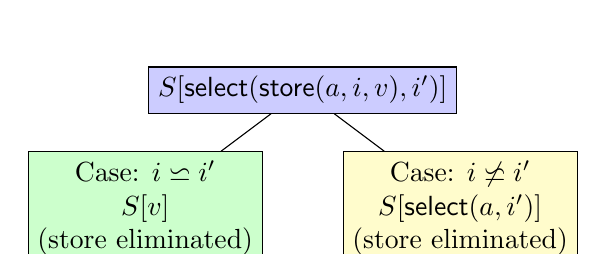
\begin{tikzpicture}[
    node distance=1.5cm and 2cm,
    every node/.style={align=center},
    level/.style={sibling distance=40mm/#1}
]
    \node[rectangle, draw, fill=blue!20] {$S[\textsf{select}(\textsf{store}(a, i, v), i')]$}
        child {node[rectangle, draw, fill=green!20] {Case: $i \backsimeq i'$\\$S[v]$\\(store eliminated)}}
        child {node[rectangle, draw, fill=yellow!20] {Case: $i \not\backsimeq i'$\\$S[\textsf{select}(a, i')]$\\(store eliminated)}};
\end{tikzpicture}
\end{center}

\begin{remark}
The procedure generates $2^n$ subproblems for $n$ occurrences of $\textsf{store}$, which can lead to exponential complexity in the worst case. However, in practice, many subproblems can be pruned early, and modern optimizations (such as lazy case splitting) significantly improve performance.
\end{remark}

\subsubsection{Correctness}

The correctness of this procedure follows from:
\begin{itemize}
    \item \textbf{Soundness}: Each subproblem correctly encodes a possible case consistent with the select-over-store axioms
    \item \textbf{Completeness}: The case splitting exhaustively covers all possibilities (either $i \backsimeq i'$ or $i \not\backsimeq i'$)
    \item \textbf{Termination}: The procedure terminates because each case split eliminates at least one $\textsf{store}$ operation, and we start with finitely many stores
\end{itemize}






\newpage

\part{Array Theory: Worked Examples}

\section{Decision Procedure Examples}

We now present four examples illustrating how the decision procedure for the theory of arrays works in practice.

\begin{example}[Satisfiability with store and inequality]
\begin{tcolorbox}[colback=green!5!white,colframe=green!75!black,title=\textbf{Example 1: SAT with Index Inequality},breakable]
\textbf{Given formula}:
\[
\textsf{select}(\textsf{store}(a, i, e), j) \backsimeq e \quad \wedge \quad i \not\backsimeq j
\]

\textbf{Question}: Is this formula satisfiable or unsatisfiable?

\vspace{0.3em}

\textbf{Intuition}: The store operation creates a new array with value $e$ at index $i$. Since $i \neq j$, it is perfectly possible for the original array $a$ to already have value $e$ at position $j$. This does not lead to a contradiction.

\vspace{0.5em}

\textbf{Decision Procedure Analysis}:

The procedure detects one occurrence of $\textsf{store}$ and performs case analysis based on whether the indices are equal:

\vspace{0.3em}

\textbf{Case 1}: $i \backsimeq j$

The formula becomes:
\[
i \backsimeq j \quad \wedge \quad e \backsimeq e \quad \wedge \quad i \not\backsimeq j
\]

\textbf{Result}: \texttt{UNSAT} — contradiction between $i \backsimeq j$ and $i \not\backsimeq j$.

\vspace{0.3em}

\textbf{Case 2}: $i \not\backsimeq j$

Applying the second select-over-store axiom:
\[
i \not\backsimeq j \quad \wedge \quad \textsf{select}(a, j) \backsimeq e
\]

Transform $\textsf{select}(a, j)$ into $f_a(j)$:
\[
i \not\backsimeq j \quad \wedge \quad f_a(j) \backsimeq e
\]

Congruence closure determines that $f_a(j)$ and $e$ are in the same equivalence class. No contradiction arises.

\textbf{Result}: \texttt{SAT}

\vspace{0.5em}

\textbf{Final Verdict}: Since at least one branch is satisfiable, the procedure returns \texttt{SAT}.
\end{tcolorbox}
\end{example}

\newpage

\begin{example}[Satisfiability with conflicting constraints]
\begin{tcolorbox}[colback=green!5!white,colframe=green!75!black,title=\textbf{Example 2: SAT with Partial Contradiction},breakable]
\textbf{Given formula}:
\[
\textsf{select}(\textsf{store}(a, i, e), j) \backsimeq e \quad \wedge \quad \textsf{select}(a, j) \not\backsimeq e
\]

\textbf{Question}: Is this formula satisfiable or unsatisfiable?

\vspace{0.5em}

\textbf{Decision Procedure Analysis}:

\textbf{Case 1}: $i \backsimeq j$

Applying the first select-over-store axiom, replace $\textsf{select}(\textsf{store}(a, i, e), j)$ with $e$:
\[
i \backsimeq j \quad \wedge \quad e \backsimeq e \quad \wedge \quad \textsf{select}(a, j) \not\backsimeq e
\]

Transform $\textsf{select}(a, j)$ into $f_a(j)$:
\[
i \backsimeq j \quad \wedge \quad e \backsimeq e \quad \wedge \quad f_a(j) \not\backsimeq e
\]

The congruence closure algorithm processes this successfully — the original array $a$ could have had any value at position $j$.

\textbf{Result}: \texttt{SAT}

\vspace{0.3em}

\textbf{Case 2}: $i \not\backsimeq j$

Applying the second select-over-store axiom:
\[
i \not\backsimeq j \quad \wedge \quad \textsf{select}(a, j) \backsimeq e \quad \wedge \quad \textsf{select}(a, j) \not\backsimeq e
\]

Direct contradiction: $\textsf{select}(a, j) \backsimeq e$ and $\textsf{select}(a, j) \not\backsimeq e$ cannot both be true.

\textbf{Result}: \texttt{UNSAT}

\vspace{0.5em}

\textbf{Final Verdict}: Since at least one branch is satisfiable (Case 1), the procedure returns \texttt{SAT}.
\end{tcolorbox}
\end{example}

\newpage

\begin{example}[Unsatisfiability on all branches]
\begin{tcolorbox}[colback=red!5!white,colframe=red!75!black,title=\textbf{Example 3: UNSAT on All Branches},breakable]
\textbf{Given formula}:
\[
\textsf{select}(\textsf{store}(a, i, e), j) \backsimeq e \quad \wedge \quad \textsf{select}(a, j) \not\backsimeq e \quad \wedge \quad i \not\backsimeq j
\]

\textbf{Question}: Is this formula satisfiable or unsatisfiable?

\vspace{0.5em}

\textbf{Decision Procedure Analysis}:

\textbf{Case 1}: $i \backsimeq j$

The formula becomes:
\[
i \backsimeq j \quad \wedge \quad \textsf{select}(\textsf{store}(a, i, e), j) \backsimeq e \quad \wedge \quad \textsf{select}(a, j) \not\backsimeq e \quad \wedge \quad i \not\backsimeq j
\]

Immediate contradiction between $i \backsimeq j$ and $i \not\backsimeq j$.

\textbf{Result}: \texttt{UNSAT}

\vspace{0.3em}

\textbf{Case 2}: $i \not\backsimeq j$

Applying the second select-over-store axiom:
\[
\textsf{select}(a, j) \backsimeq e \quad \wedge \quad \textsf{select}(a, j) \not\backsimeq e \quad \wedge \quad i \not\backsimeq j
\]

Direct contradiction between $\textsf{select}(a, j) \backsimeq e$ and $\textsf{select}(a, j) \not\backsimeq e$.

\textbf{Result}: \texttt{UNSAT}

\vspace{0.5em}

\textbf{Final Verdict}: Since both branches are unsatisfiable, the procedure returns \texttt{UNSAT}.
\end{tcolorbox}
\end{example}

\newpage

\begin{example}[Nested store operations]
\begin{tcolorbox}[colback=red!5!white,colframe=red!75!black,title=\textbf{Example 4: UNSAT with Nested Stores},breakable]
\textbf{Given formula}:
\begin{align*}
i_1 \backsimeq j \quad &\wedge \quad i_1 \not\backsimeq i_2 \quad \wedge \quad \textsf{select}(a, j) \backsimeq v_1 \\
&\wedge \quad \textsf{select}(\textsf{store}(\textsf{store}(a, i_1, v_1), i_2, v_2), j) \not\backsimeq \textsf{select}(a, j)
\end{align*}

\textbf{Question}: Is this formula satisfiable or unsatisfiable?

\vspace{0.5em}

\textbf{Decision Procedure Analysis}:

The formula involves nested $\textsf{store}$ operations. We perform case analysis on whether $j \backsimeq i_2$:

\vspace{0.3em}

\textbf{Case 1}: $j \backsimeq i_2$

Applying the first select-over-store axiom (since $j \backsimeq i_2$):
\begin{align*}
i_1 \backsimeq j \quad &\wedge \quad i_1 \not\backsimeq i_2 \quad \wedge \quad j \backsimeq i_2 \quad \wedge \quad \textsf{select}(a, j) \backsimeq v_1 \\
&\wedge \quad v_2 \not\backsimeq \textsf{select}(a, j)
\end{align*}

Transform $\textsf{select}(a, j)$ into $f_a(j)$:
\[
i_1 \backsimeq j \quad \wedge \quad i_1 \not\backsimeq i_2 \quad \wedge \quad j \backsimeq i_2 \quad \wedge \quad f_a(j) \backsimeq v_1 \quad \wedge \quad v_2 \not\backsimeq f_a(j)
\]

Congruence closure returns \texttt{UNSAT}: we have $i_1 \backsimeq j \backsimeq i_2$ but $i_1 \not\backsimeq i_2$ (contradiction).

\textbf{Result}: \texttt{UNSAT}

\vspace{0.3em}

\textbf{Case 2}: $j \not\backsimeq i_2$

Applying the second select-over-store axiom:
\begin{align*}
i_1 \backsimeq j \quad &\wedge \quad i_1 \not\backsimeq i_2 \quad \wedge \quad \textsf{select}(a, j) \backsimeq v_1 \\
&\wedge \quad \textsf{select}(\textsf{store}(a, i_1, v_1), j) \not\backsimeq \textsf{select}(a, j)
\end{align*}

Now we need a second case analysis on whether $j \backsimeq i_1$. However, we already have $i_1 \backsimeq j$ as part of the problem, so the branch $j \not\backsimeq i_1$ is immediately unsatisfiable.

\textbf{Subcase 2.1}: $j \backsimeq i_1$ (forced by the given constraint)

Applying the first select-over-store axiom:
\[
i_1 \backsimeq j \quad \wedge \quad i_1 \not\backsimeq i_2 \quad \wedge \quad \textsf{select}(a, j) \backsimeq v_1 \quad \wedge \quad v_1 \not\backsimeq \textsf{select}(a, j)
\]

Direct contradiction: $\textsf{select}(a, j) \backsimeq v_1$ and $v_1 \not\backsimeq \textsf{select}(a, j)$ cannot both be true.

\textbf{Result}: \texttt{UNSAT}

\vspace{0.5em}

\textbf{Final Verdict}: Since all branches are unsatisfiable, the procedure returns \texttt{UNSAT}.
\end{tcolorbox}
\end{example} 



\newpage 

\part{Theory Combination: Exercises and Assumptions}

\section{Exercise}

\begin{example}[Theory Combination Exercise]
Consider the formula:
\[
1 \leq x \wedge x \leq 2 \wedge f(x) \not\backsimeq f(1) \wedge f(x) \not\backsimeq f(2)
\]

\textbf{Analysis with different theories}:

\begin{itemize}
    \item $\mathcal{T}_E \cup \mathcal{T}_{\text{LRA}}$ (Linear Rational Arithmetic) $\longrightarrow$ \texttt{SAT}

    Satisfying assignment: $x \leftarrow 0.5$

    \item $\mathcal{T}_E \cup \mathcal{T}_{\text{LIA}}$ (Linear Integer Arithmetic) $\longrightarrow$ \texttt{UNSAT}
\end{itemize}

\textbf{Key observation}: In $\mathcal{T}_E$, from $x \backsimeq 1 \vee x \backsimeq 2$ we can deduce $f(x) \backsimeq f(1)$ (by congruence).
\end{example}

\section{The Nelson-Oppen Scheme for Theory Combination}

The Nelson-Oppen scheme is an \textbf{equality-sharing scheme} for combining theories.

\subsection{Assumptions}

\begin{tcolorbox}[colback=blue!5!white,colframe=blue!75!black,title=\textbf{Nelson-Oppen Assumptions}]
\textbf{Assumption 1: Decision Procedures}

Each theory $\mathcal{T}_i$ has a decision procedure for the satisfiability of sets (conjunctions) of $\mathcal{T}_i$-literals.

Combining theories by combining procedures as black-boxes.

\vspace{0.5em}

\textbf{Assumption 2: Disjoint Signatures}

The theories are pairwise disjoint, i.e., the only shared symbol is $\backsimeq$ (equality).

\begin{itemize}
    \item It's ok if they share sorts and variables (and hence also constants, because variables and constants are interchangeable in the quantifier-free fragment)
    \item They cannot share function or predicate symbols
\end{itemize}

Example:
\begin{align*}
f &\in \Sigma_E \\
1, 2, < &\in \Sigma_{\text{Arithm}} \\
\backsimeq &\in \Sigma_E \cap \Sigma_{\text{Arithm}}
\end{align*}

The theories will have to agree only about $\backsimeq$.

\vspace{0.5em}

\textbf{Assumption 3: Stable Infiniteness}

The theories are \textbf{stably infinite}, i.e., each theory $\mathcal{T}_i$ has models where all the sorts are interpreted as countably infinite sets.

The theories agree upfront on the cardinality of the shared sorts (by making them all infinite).
\end{tcolorbox}

\subsection{Architecture}

\begin{center}
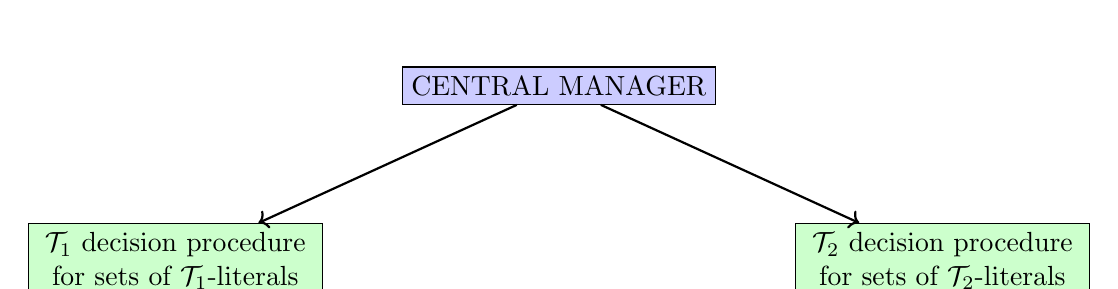
\begin{tikzpicture}[node distance=2cm]
    \node[rectangle, draw, fill=blue!20] (cm) {CENTRAL MANAGER};
    \node[rectangle, draw, fill=green!20, below left=1.5cm and 1cm of cm, text width=3.5cm, align=center] (t1) {$\mathcal{T}_1$ decision procedure \\ for sets of $\mathcal{T}_1$-literals};
    \node[rectangle, draw, fill=green!20, below right=1.5cm and 1cm of cm, text width=3.5cm, align=center] (t2) {$\mathcal{T}_2$ decision procedure \\ for sets of $\mathcal{T}_2$-literals};
    \draw[->,thick] (cm) -- (t1);
    \draw[->,thick] (cm) -- (t2);
\end{tikzpicture}
\end{center}

\subsection{Phase I: Separation}

Separate and decompose the problem.

\begin{example}[Separation Example]
Given:
\[
1 \leq x \wedge x \leq 2 \wedge f(x) \not\backsimeq f(1) \wedge f(x) \not\backsimeq f(2)
\]

After separation into $\mathcal{T}_E$ and $\mathcal{T}_{\text{Arithm}}$:
\begin{align*}
F_E &: f(x) \not\backsimeq f(w_2) \wedge f(x) \not\backsimeq f(w_1) \\
F_{\text{Arithm}} &: 1 \leq x \wedge x \leq 2 \wedge w_1 \backsimeq 1 \wedge w_2 \backsimeq 2
\end{align*}

Shared variables: $V = \{w_1, x, w_2\}$
\end{example}

\subsubsection{Separation Rules}

When we have $[t[s]]$ where the top symbol of $s$ belongs to $\Sigma_i$ and $t$ to $\Sigma_j$:
\begin{align*}
F_1 &: L[t[w]] \\
F_2 &: w \backsimeq s
\end{align*}

When we have $t_1 \backsimeq t_2$ where the top symbol of $t_1$ belongs to $\Sigma_i$ and the top of $t_2$ belongs to $\Sigma_j$ ($i \neq j$), we introduce a fresh variable.

\begin{tcolorbox}[colback=green!5!white,colframe=green!75!black,title=\textbf{Separation Process}]
\textbf{Input} $F$: set of $\mathcal{T}_1 \cup \mathcal{T}_2$ literals

\textbf{After separation}: $F_1$ and $F_2$
\begin{itemize}
    \item $F_1$: set of $\mathcal{T}_1$-literals
    \item $F_2$: set of $\mathcal{T}_2$-literals
\end{itemize}

\textbf{Key property}: $F$ is $\mathcal{T}_1 \cup \mathcal{T}_2$-satisfiable if and only if $F_1 \cup F_2$ is $\mathcal{T}_1 \cup \mathcal{T}_2$-satisfiable.
\end{tcolorbox}

\subsection{Phase II: Arrangements}

Work on the shared variables and $\backsimeq$.

Find an arrangement of the set $V$ of shared variables.

\newpage


\part{Nelson-Oppen Scheme}

\section{Combining Decision Procedures}

\subsection{Introduction to the Nelson-Oppen Scheme}

The \textbf{Nelson-Oppen scheme} provides a method for combining $\mathcal{T}_i$-decision procedures where $i \in \{1, 2\}$.

The procedure is organized with a \textbf{central manager} (C.M.) which is responsible for the communication between the two decision procedures. We don't want to modify the procedures, just combine them as black-boxes.

\begin{center}
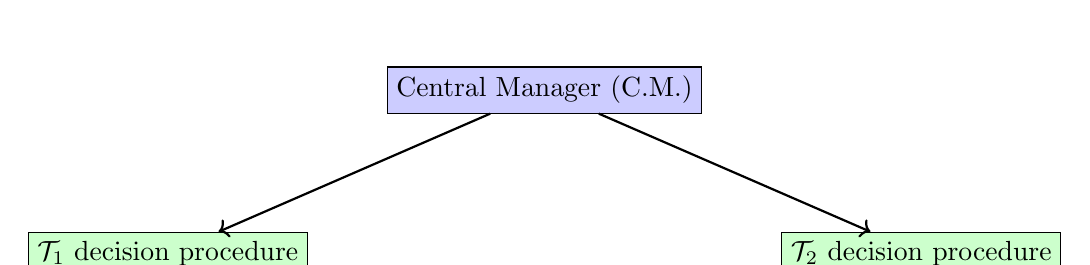
\begin{tikzpicture}[node distance=2cm]
    \node[rectangle, draw, fill=blue!20] (cm) {Central Manager (C.M.)};
    \node[rectangle, draw, fill=green!20, below left=1.5cm and 1cm of cm] (t1) {$\mathcal{T}_1$ decision procedure};
    \node[rectangle, draw, fill=green!20, below right=1.5cm and 1cm of cm] (t2) {$\mathcal{T}_2$ decision procedure};
    \draw[->,thick] (cm) -- (t1);
    \draw[->,thick] (cm) -- (t2);
\end{tikzpicture}
\end{center} 

\subsection{Phase I: Separation}

The first phase of the scheme is called \textbf{Separation}.

\begin{tcolorbox}[colback=blue!5!white,colframe=blue!75!black,title=\textbf{Separation Phase}]
The separation phase separates the input into two sets:
\[
F \longrightarrow F_1 \wedge F_2
\]

where:
\begin{itemize}
    \item $F$ is a set of mixed $\mathcal{T}_1 \cup \mathcal{T}_2$ literals
    \item $F_i$ is the set of $\mathcal{T}_i$-literals only
\end{itemize}

\textbf{Key property}: $F$ is $\mathcal{T}_1 \cup \mathcal{T}_2$-satisfiable if and only if $F_1 \wedge F_2$ is $\mathcal{T}_1 \cup \mathcal{T}_2$-satisfiable.
\end{tcolorbox}

\subsubsection{Separation Rules}

Let $w$ be a new variable. The separation is performed according to the following rules:

\begin{enumerate}
    \item If $\text{head}(t) \in \Sigma_j$ and $f \in \Sigma_i$ with $j \neq i$:
    \[
    F[f(t_1, \ldots, t, \ldots, t_n)] \longrightarrow F[f(t_1, \ldots, w, \ldots, t_n)] \wedge w \backsimeq t
    \]

    \item If $\text{head}(t) \in \Sigma_j$ and $P \in \Sigma_i$ with $j \neq i$ (where $P$ can also be equality $\backsimeq$):
    \[
    F[P(t_1, \ldots, t, \ldots, t_n)] \longrightarrow F[P(t_1, \ldots, w, \ldots, t_n)] \wedge w \backsimeq t
    \]

    \item If $\text{head}(s) \in \Sigma_i$ and $\text{head}(t) \in \Sigma_j$:
    \[
    F[\ldots] \wedge s \backsimeq t \longrightarrow F[\ldots] \wedge s \backsimeq w \wedge w \backsimeq t
    \]
\end{enumerate}

\begin{example}[Simple Separation]
Consider:
\[
f(2, y) \backsimeq f(x, y)
\]

This is a combination of theories because $f \in \Sigma_{\text{Equality}}$ and $2 \in \Sigma_{\mathbb{Z}}$ (arithmetic).

We create $F_E$ and $F_{\mathbb{Z}}$:
\begin{align*}
F_E &: f(w, y) \backsimeq f(x, y) \\
F_{\mathbb{Z}} &: w \backsimeq 2
\end{align*}
\end{example} 

\begin{example}[Complex Separation]
Consider:
\[
F: x \leq y \wedge y \leq (x + g(x)) \wedge P(h(x) - h(y)) \wedge \neg P(0) \wedge g(x) \backsimeq 0
\]

where $x$ is some kind of number (for the $+$ symbol), $g$ is a function that takes an integer and returns an integer (integers or rational numbers); if $x$ is a number, also $y$ must be a number; $h$ is like $g$, a function (although it operates on numbers and returns numbers); $P$ is a predicate which applies also to numbers.

This is a combination between:
\[
\mathcal{T}_{\mathbb{Z}} \cup \mathcal{T}_E
\]

where $\mathcal{T}_{\mathbb{Z}}$ is the theory of integers $\{\leq, +, -, 0\}$ and $\mathcal{T}_E$ is the theory of equality $\{f, g, h, P\}$.

We could also interpret $\mathcal{T}_{\mathbb{Z}}$ as the theory of rationals $\mathcal{T}_{\mathbb{Q}}$ (these integers could actually also be rationals).

\textbf{How can we separate}:
\begin{align*}
F_{\mathbb{Z}} &: x \leq y \wedge y \leq (x + w_1) \wedge w_2 \backsimeq w_3 - w_4 \wedge w_5 \backsimeq 0 \\
F_E &: w_1 \backsimeq g(x) \wedge P(w_2) \wedge w_3 \backsimeq h(x) \wedge w_4 \backsimeq h(y) \wedge \neg P(w_5) \wedge g(x) \backsimeq w_5
\end{align*}

\textbf{Set of shared variables}:
\[
V = \{x, y, w_1, w_2, w_3, w_4, w_5\}
\]

We rewrite the problem (rewriting $P$ as $f_P$):
\[
F_E: w_1 \backsimeq g(x) \wedge f_P(w_2) \backsimeq \bullet \wedge w_3 \backsimeq h(x) \wedge w_4 \backsimeq h(y) \wedge f_P(w_5) \not\backsimeq \bullet \wedge g(x) \backsimeq w_5
\]
\end{example} 

\subsection{Phase II: Arrangements}

Two procedures decide $\mathcal{T}_1$-SAT and $\mathcal{T}_2$-SAT: but not $\mathcal{T}_1 \cup \mathcal{T}_2$-SAT.

Here comes the notion of \textbf{arrangement} of the set $V$ of shared variables.

An arrangement will have to do with equality (the \textit{only} shared symbol in the 2 theories, all other symbols make sense only in 1 of the 2 theories). It will say which shared variables are equal and which are not.

\subsubsection{Arrangements and Equivalence Relations}

We have a set $V$ of shared variables:
\[
V = \{x, y, w_1, w_2, w_3, w_4, w_5\}
\]

Here we are considering equality between variables (no function symbols), so an equivalence is sufficient.

We are interested in an equivalence relation over the set $V$ of shared variables:
\[
E \subseteq V \times V
\]

We know that an equivalence relation generates a partition. We are looking for the partition of the set $E$ of shared variables.

\begin{tcolorbox}[colback=teal!10!white,colframe=teal!75!black,title=\textbf{Arrangement Definition}]
We define an \textbf{arrangement} $\alpha(V, E)$ as a conjunction of equalities and disequalities:
\[
\alpha(V, E) = \bigwedge_{\substack{u, v \in V \\ u \, E \, v}} u \backsimeq v \quad \wedge \quad \bigwedge_{\substack{u, v \in V \\ \neg(u \, E \, v)}} u \not\backsimeq v
\]
\end{tcolorbox}

\textbf{Phase II goal}: Find an $\alpha(V, E)$ such that:
\[
F_1 \wedge F_2 \text{ is } \mathcal{T}_1 \cup \mathcal{T}_2\text{-satisfiable iff } F_1 \wedge \alpha(V, E) \text{ is } \mathcal{T}_1\text{-satisfiable and } F_2 \wedge \alpha(V, E) \text{ is } \mathcal{T}_2\text{-satisfiable}
\] 

\subsection{Non-Deterministic Nelson-Oppen Scheme}

\textbf{How to look for $\alpha$?}

The non-deterministic version of the Nelson-Oppen scheme is simply based on:
\begin{itemize}
    \item Guess $E$ and hence $\alpha(V, E)$
    \item Check the $\mathcal{T}_1$-satisfiability and the $\mathcal{T}_2$-satisfiability of $F_1 \wedge \alpha(V, E)$ and $F_2 \wedge \alpha(V, E)$ respectively
\end{itemize}

Enumerate all possible $E$ and test them:
\begin{itemize}
    \item As soon as one succeeds (both problems return \texttt{SAT}), we return \texttt{SAT}
    \item If none succeeds (at least one returns \texttt{UNSAT}), we return \texttt{UNSAT}
\end{itemize}

\begin{example}[Non-Deterministic Nelson-Oppen]
Consider:
\[
f(x) \backsimeq x + y \wedge x \leq y + z \wedge x + z \leq y \wedge y \backsimeq 1 \wedge f(x) \not\backsimeq f(2)
\]

After separation:
\begin{align*}
F_E &: f(x) \backsimeq w_1 \wedge f(x) \not\backsimeq f(w_2) \\
F_{\mathbb{Z}} &: w_1 \backsimeq x + y \wedge x \leq y + z \wedge x + z \leq y \wedge y \backsimeq 1 \wedge w_2 \backsimeq 2
\end{align*}

Set of shared variables:
\[
V = \{w_1, w_2, x\}
\]

Try different equivalence relations:
\begin{itemize}
    \item $E_0: \{\{w_1\}, \{w_2\}, \{x\}\}$ \\
    $\alpha(E_0, V) = w_1 \not\backsimeq w_2 \wedge w_1 \not\backsimeq x \wedge w_2 \not\backsimeq x$ $\longrightarrow$ \texttt{SAT}

    \item $E_1: \{\{w_1\}, \{w_2, x\}\}$ \\
    $\alpha(E_1, V) = w_2 \backsimeq x \wedge w_1 \not\backsimeq w_2 \wedge w_1 \not\backsimeq x$ $\longrightarrow$ \texttt{CONTRADICTION}
\end{itemize}
\end{example}

\begin{remark}
For $|V| = n$, the number of equivalence relations is equal to $\text{Bell}(n)$.

Bell numbers are a sequence of integers which capture exactly the number of equivalence relations that exist over a set of $n$ elements.
\end{remark} 

\subsection{Deterministic Nelson-Oppen Scheme}

In the deterministic Nelson-Oppen scheme, we don't guess $E$ and $\alpha(V, E)$, but we build incrementally $E$ and $\alpha(V, E)$ in the arrangement.

This is the one used in practice.

\subsubsection{Convexity Property}

We need to verify the theories have all the property of \textbf{Convexity}.

\begin{tcolorbox}[colback=purple!5!white,colframe=purple!75!black,title=\textbf{Convexity Definition}]
A theory $\mathcal{T}$ is \textbf{convex} if and only if:
\[
\mathcal{T} \models H \rightarrow \bigvee_{k=1}^{n} u_k \backsimeq v_k \quad \Rightarrow \quad \exists q, \, 1 \leq q \leq n, \text{ such that } \mathcal{T} \models H \rightarrow u_q \backsimeq v_q
\]

where:
\begin{itemize}
    \item $u_k, v_k$ are variables
    \item $H$ is a conjunction of $\mathcal{T}$-literals
\end{itemize}
\end{tcolorbox}

If a theory is convex we don't need to reason about disjunction.

\begin{center}
\textbf{Examples of Convex and Non-Convex Theories}
\end{center}

\textbf{Convex theories}:
\begin{itemize}
    \item $\mathcal{T}_E$ (theory of equality)
    \item $\mathcal{T}_{\text{cons}}$ (theory of lists/constructors)
    \item $\mathcal{T}_{\mathbb{Q}}$ (theory of rationals)
\end{itemize}

\textbf{Non-convex theories}:
\begin{itemize}
    \item $\mathcal{T}_{\mathbb{Z}}$ (theory of integers)
    \item $\mathcal{T}_A$ (theory of arrays)
\end{itemize} 

\subsubsection{Two Versions of the Deterministic Scheme}

We need 2 versions of the deterministic scheme:

\begin{enumerate}
    \item \textbf{If $\mathcal{T}_1$ and $\mathcal{T}_2$ are convex}: \\
    It suffices that the $\mathcal{T}_i$-procedure (where $i$ can be 1 or 2) is capable of deducing all equalities between shared variables $\mathcal{T}_i$-entailed by $F_i$.

    \item \textbf{If a theory $\mathcal{T}_i$ is not convex}: \\
    The $\mathcal{T}_i$-procedure must be capable of deducing all disjunctions of equalities between shared variables $\mathcal{T}_i$-entailed by $F_i$.
\end{enumerate}

\subsubsection{Deterministic Algorithm for Convex Theories}

\begin{tcolorbox}[colback=green!5!white,colframe=green!75!black,title=\textbf{Deterministic Nelson-Oppen Algorithm}]
Let $\mathcal{E}$ be the set of shared equalities between shared variables.

\textbf{Initialization}: $\mathcal{E} = \emptyset$

\textbf{Iteration}:
\begin{enumerate}
    \item Suppose $P_i$ (decision procedure for $\mathcal{T}_i$) finds that:
    \[
    F_i \cup \mathcal{E} \models_{\mathcal{T}_i} x \backsimeq y \quad \text{where } x, y \in V
    \]
    Then it sends it to the central manager (C.M.).

    \item Update:
    \[
    \mathcal{E}_{k+1} = \mathcal{E}_k \cup \{x \backsimeq y\}
    \]
    We add to the set of shared equalities the new one that we have discovered.

    \item Then, maybe $P_j$ also finds that:
    \[
    F_j \cup \mathcal{E}_{k+1} \models_{\mathcal{T}_j} x \backsimeq y \quad \text{where } x, y \in V
    \]
    \[
    \mathcal{E}_{k+2} = \mathcal{E}_{k+1} \cup \{x \backsimeq y\}
    \]
\end{enumerate}

\textbf{Termination}:
\begin{itemize}
    \item \textbf{Termination 1}: When neither $P_i$ nor $P_j$ can deduce any more equalities between shared variables $\longrightarrow$ return \texttt{SAT}
    \item \textbf{Termination 2}: When $P_i$ or $P_j$ deduces contradictions $\longrightarrow$ return \texttt{UNSAT}
\end{itemize}
\end{tcolorbox}


\newpage

\part{Nelson-Oppen: Worked Examples}

\section{Deterministic Nelson-Oppen Exercises}

In this section, we present detailed examples of applying the deterministic Nelson-Oppen scheme. We have already seen examples of the first phase (Separation), now we focus on complete exercises including the second phase (Arrangements).

\begin{example}[Deterministic Nelson-Oppen with Convex Theories]
\begin{tcolorbox}[colback=blue!5!white,colframe=blue!75!black,title=\textbf{Example 1: Combining $\mathcal{T}_E$ and $\mathcal{T}_{\text{LIA}}$},breakable]
\textbf{Given formula}:
\[
f(x) \backsimeq x + y \quad \wedge \quad x \leq y + z \quad \wedge \quad x + z \leq y \quad \wedge \quad y \backsimeq 1 \quad \wedge \quad f(x) \not\backsimeq f(2)
\]

\textbf{Question}: Is this formula satisfiable or unsatisfiable?

\vspace{0.5em}

\textbf{Step 1: Identify the theories involved}

First, we identify which theories are involved:
\begin{itemize}
    \item $\mathcal{T}_E$ (Theory of Equality with uninterpreted functions) — because of function symbol $f$
    \item $\mathcal{T}_{\text{LIA}}$ (Linear Integer Arithmetic) — because of arithmetic operations and constraints
\end{itemize}

\vspace{0.5em}

\textbf{Step 2: Separation Phase}

We separate the formula into $F_E$ and $F_{\text{LIA}}$:

\begin{align*}
F_E &: f(x) \backsimeq w_1 \quad \wedge \quad f(x) \not\backsimeq f(w_2) \\
F_{\text{LIA}} &: w_1 \backsimeq x + y \quad \wedge \quad x \leq y + z \quad \wedge \quad x + z \leq y \quad \wedge \quad y \backsimeq 1 \quad \wedge \quad w_2 \backsimeq 2
\end{align*}

\textbf{Set of shared variables}:
\[
V = \{w_1, w_2, x, y, z\}
\]

\vspace{0.5em}

\textbf{Step 3: Deterministic Nelson-Oppen — Arrangement Phase}

We now apply the deterministic Nelson-Oppen algorithm. The two decision procedures (congruence closure for $\mathcal{T}_E$ and simplex for $\mathcal{T}_{\text{LIA}}$) will communicate by sharing equalities between variables in $V$.

\textbf{Initial state}: $\mathcal{E}_0 = \emptyset$

\vspace{0.3em}

\textbf{Analysis of $F_{\text{LIA}}$}:

From the arithmetic constraints, we can derive information about the shared variables. Let's analyze what the arithmetic procedure can deduce.

From the constraints $x \leq y + z$ and $x + z \leq y$, we can derive:
\begin{align*}
x - y &\leq z \tag{from $x \leq y + z$} \\
x - y &\leq -z \tag{from $x + z \leq y$}
\end{align*}

Adding these two inequalities:
\begin{align*}
(x - y) + (x - y) &\leq z + (-z) \\
2x - 2y &\leq 0 \\
2x &\leq 2y \\
x &\leq y
\end{align*}

Since $y \backsimeq 1$, we can conclude:
\[
x \leq 1
\]

Also, from $y \backsimeq 1$ and $w_1 \backsimeq x + y$:
\[
w_1 \backsimeq x + 1
\]

This means $w_1 \not\backsimeq x$ (since $w_1 = x + 1 \neq x$).

Similarly, $w_2 \backsimeq 2$ and $x \leq 1$ imply $x \not\backsimeq w_2$.

\vspace{0.3em}

\textbf{Analysis of $F_E$}:

From $f(x) \not\backsimeq f(w_2)$, the congruence closure algorithm cannot deduce any equality between shared variables (only that $x \not\backsimeq w_2$, but this is a disequality).

\vspace{0.3em}

\textbf{Iteration}: No new equalities between shared variables are propagated

Neither procedure finds equalities between shared variables that need to be propagated to the other procedure. The algorithm terminates without finding a contradiction.

\vspace{0.5em}

\textbf{Step 4: Satisfying Assignment}

Since no contradiction was found, the formula is \texttt{SAT}. We can construct a satisfying assignment:

\begin{align*}
x &\leftarrow 0 \\
y &\leftarrow 1 \\
z &\leftarrow 0 \\
w_1 &\leftarrow 1 \quad \text{(since $w_1 = x + y = 0 + 1 = 1$)} \\
w_2 &\leftarrow 2 \\
f(0) &\leftarrow 1 \\
f(2) &\leftarrow \text{any value different from } 1
\end{align*}

We can verify this assignment satisfies all constraints:
\begin{itemize}
    \item $f(x) \backsimeq x + y$: $f(0) = 1 = 0 + 1$ \checkmark
    \item $x \leq y + z$: $0 \leq 1 + 0$ \checkmark
    \item $x + z \leq y$: $0 + 0 \leq 1$ \checkmark
    \item $y \backsimeq 1$: $1 = 1$ \checkmark
    \item $f(x) \not\backsimeq f(2)$: $f(0) = 1 \neq f(2)$ \checkmark
\end{itemize}

\vspace{0.5em}

\textbf{Final Answer}: The formula is \texttt{SAT}.
\end{tcolorbox}
\end{example} 

\newpage

\begin{example}[Deterministic Nelson-Oppen with Fourier-Motzkin]
\begin{tcolorbox}[colback=blue!5!white,colframe=blue!75!black,title=\textbf{Example 2: UNSAT with Equality Propagation},breakable]
\textbf{Given formula}:
\[
f(f(x) - f(y)) \not\backsimeq f(z) \quad \wedge \quad x \leq y \quad \wedge \quad y + z \leq x \quad \wedge \quad 0 \leq z
\]

\textbf{Question}: Is this formula satisfiable or unsatisfiable?

\vspace{0.5em}

\textbf{Step 1: Identify the theories involved}

Again, we have a combination of two theories:
\begin{itemize}
    \item $\mathcal{T}_E$ (Theory of Equality with uninterpreted functions) — because of function symbol $f$
    \item $\mathcal{T}_{\text{LIA}}$ (Linear Integer Arithmetic) — because of arithmetic operations and inequality constraints
\end{itemize}

Note: We could also use $\mathcal{T}_{\text{LRA}}$ (Linear Rational Arithmetic) instead, as the constraints don't require integrality.

\vspace{0.5em}

\textbf{Step 2: Separation Phase}

We separate the formula into $F_E$ and $F_{\text{LIA}}$:

\begin{align*}
F_E &: f(w_1) \not\backsimeq f(z) \quad \wedge \quad w_2 \backsimeq f(x) \quad \wedge \quad w_3 \backsimeq f(y) \\
F_{\text{LIA}} &: w_1 \backsimeq w_2 - w_3 \quad \wedge \quad x \leq y \quad \wedge \quad y + z \leq x \quad \wedge \quad 0 \leq z
\end{align*}

\textbf{Set of shared variables}:
\[
V = \{w_1, w_2, w_3, x, y, z\}
\]

\vspace{0.5em}

\textbf{Step 3: Deterministic Nelson-Oppen — Arrangement Phase}

We apply the deterministic Nelson-Oppen algorithm with equality sharing.

\textbf{Initial state}: $\mathcal{E}_0 = \emptyset$

\vspace{0.3em}

\textbf{Fourier-Motzkin Elimination Background}:

Before proceeding, recall the Fourier-Motzkin resolution rule used in linear arithmetic:
\[
\frac{t_1 \prec_1 z \quad z \prec_2 t_2}{t_1 \prec_3 t_2}
\]
where:
\begin{itemize}
    \item $t_1, t_2$ are linear arithmetic terms (not containing variable $z$)
    \item $z$ is a variable to be eliminated
    \item $\prec_1, \prec_2, \prec_3 \in \{<, \leq\}$
\end{itemize}

This rule allows us to eliminate variables and derive relationships between other terms.

\vspace{0.3em}

\textbf{Iteration 1: Arithmetic procedure deduces $x \backsimeq y$}

From $F_{\text{LIA}}$, we have:
\begin{align*}
x &\leq y \\
y + z &\leq x \\
0 &\leq z
\end{align*}

From $y + z \leq x$, we get $y \leq x - z$. Combined with $0 \leq z$, we have $y \leq x$.

But we also have $x \leq y$. Therefore:
\[
x \leq y \quad \wedge \quad y \leq x \quad \Rightarrow \quad x \backsimeq y
\]

The arithmetic procedure sends this equality to the central manager:
\[
\mathcal{E}_1 = \{x \backsimeq y\}
\]

\vspace{0.3em}

\textbf{Iteration 2: Equality procedure deduces $w_2 \backsimeq w_3$}

The congruence closure procedure receives $x \backsimeq y$ and processes:
\begin{align*}
x \backsimeq y &\models_{\mathcal{T}_E} f(x) \backsimeq f(y) \quad \text{(by congruence)} \\
w_2 \backsimeq f(x) \wedge w_3 \backsimeq f(y) &\models_{\mathcal{T}_E} w_2 \backsimeq w_3 \quad \text{(by transitivity)}
\end{align*}

The equality procedure sends this to the central manager:
\[
\mathcal{E}_2 = \{x \backsimeq y, w_2 \backsimeq w_3\}
\]

\vspace{0.3em}

\textbf{Iteration 3: Arithmetic procedure deduces $w_1 \backsimeq 0$}

The arithmetic procedure receives $w_2 \backsimeq w_3$ and processes:
\begin{align*}
w_1 &\backsimeq w_2 - w_3 \quad \text{(from $F_{\text{LIA}}$)} \\
w_2 &\backsimeq w_3 \quad \text{(received from equality)} \\
\Rightarrow w_1 &\backsimeq w_2 - w_2 \\
\Rightarrow w_1 &\backsimeq 0
\end{align*}

The arithmetic procedure sends this to the central manager:
\[
\mathcal{E}_3 = \{x \backsimeq y, w_2 \backsimeq w_3, w_1 \backsimeq 0\}
\]

\vspace{0.3em}

\textbf{Iteration 4: Equality procedure detects contradiction}

The congruence closure procedure receives $w_1 \backsimeq 0$ and analyzes:

From $F_E$, we have $f(w_1) \not\backsimeq f(z)$.

Now we need to check if $w_1 \backsimeq z$ or $w_1 \not\backsimeq z$.

Going back to the arithmetic constraints with $x \backsimeq y$ and $w_1 \backsimeq 0$:
\begin{align*}
x &\backsimeq y \\
y + z &\leq x \\
\Rightarrow y + z &\leq y \quad \text{(substituting $x$ with $y$)} \\
\Rightarrow z &\leq 0
\end{align*}

Combined with $0 \leq z$, we get:
\[
z \leq 0 \quad \wedge \quad 0 \leq z \quad \Rightarrow \quad z \backsimeq 0
\]

The arithmetic procedure sends $z \backsimeq 0$ to the central manager:
\[
\mathcal{E}_4 = \{x \backsimeq y, w_2 \backsimeq w_3, w_1 \backsimeq 0, z \backsimeq 0\}
\]

Now the congruence closure procedure has:
\begin{align*}
w_1 &\backsimeq 0 \\
z &\backsimeq 0 \\
\Rightarrow w_1 &\backsimeq z \quad \text{(by transitivity)}
\end{align*}

By congruence:
\[
w_1 \backsimeq z \quad \models_{\mathcal{T}_E} \quad f(w_1) \backsimeq f(z)
\]

But from $F_E$, we have $f(w_1) \not\backsimeq f(z)$.

\textbf{CONTRADICTION!}

\vspace{0.5em}

\textbf{Final Answer}: The formula is \texttt{UNSAT}.

\vspace{0.3em}

\textbf{Summary of the propagation chain}:
\begin{center}
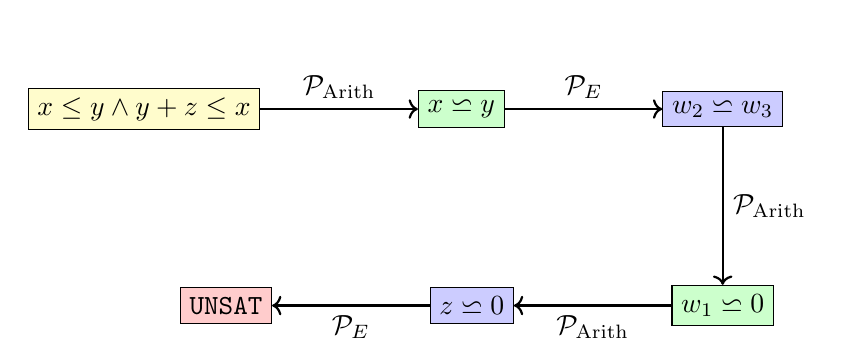
\begin{tikzpicture}[node distance=2cm, auto]
    \node[rectangle, draw, fill=yellow!20] (start) {$x \leq y \wedge y+z \leq x$};
    \node[rectangle, draw, fill=green!20, right=of start] (eq1) {$x \backsimeq y$};
    \node[rectangle, draw, fill=blue!20, right=of eq1] (eq2) {$w_2 \backsimeq w_3$};
    \node[rectangle, draw, fill=green!20, below=of eq2] (eq3) {$w_1 \backsimeq 0$};
    \node[rectangle, draw, fill=blue!20, left=of eq3] (eq4) {$z \backsimeq 0$};
    \node[rectangle, draw, fill=red!20, left=of eq4] (unsat) {\texttt{UNSAT}};

    \draw[->,thick] (start) -- node {$\mathcal{P}_{\text{Arith}}$} (eq1);
    \draw[->,thick] (eq1) -- node {$\mathcal{P}_E$} (eq2);
    \draw[->,thick] (eq2) -- node {$\mathcal{P}_{\text{Arith}}$} (eq3);
    \draw[->,thick] (eq3) -- node {$\mathcal{P}_{\text{Arith}}$} (eq4);
    \draw[->,thick] (eq4) -- node {$\mathcal{P}_E$} (unsat);
\end{tikzpicture}
\end{center}
\end{tcolorbox}
\end{example}

\newpage

\begin{example}[Non-Convex Theory: Disjunctive Reasoning]
\begin{tcolorbox}[colback=purple!5!white,colframe=purple!75!black,title=\textbf{Example 3: Non-Convex $\mathcal{T}_{\text{LIA}}$ with Disjunctions},breakable]
\textbf{Given formula}:
\[
1 \leq x \quad \wedge \quad x \leq 2 \quad \wedge \quad f(x) \not\backsimeq f(1) \quad \wedge \quad f(x) \not\backsimeq f(2)
\]

\textbf{Question}: Is this formula satisfiable or unsatisfiable?

\vspace{0.5em}

\textbf{Key observation}: This is the classic example we saw earlier that illustrates the importance of \textbf{stable infiniteness} and demonstrates non-convex theory behavior.

\vspace{0.3em}

\textbf{Expected results}:
\begin{itemize}
    \item Using $\mathcal{T}_E \cup \mathcal{T}_{\text{LIA}}$ (Linear Integer Arithmetic): \textbf{UNSAT}
    \item Using $\mathcal{T}_E \cup \mathcal{T}_{\text{LRA}}$ (Linear Rational Arithmetic): \textbf{SAT}

    For $\mathcal{T}_{\text{LRA}}$, we can satisfy with $x \leftarrow 1.5$ (or any value in the open interval $(1, 2)$).
\end{itemize}

\vspace{0.5em}

We will analyze the case with \textbf{integer arithmetic} to demonstrate how the deterministic Nelson-Oppen scheme handles \textbf{non-convex theories}.

\vspace{0.5em}

\textbf{Step 1: Identify the theories involved}

\begin{itemize}
    \item $\mathcal{T}_E$ (Theory of Equality) — \textbf{convex}
    \item $\mathcal{T}_{\text{LIA}}$ (Linear Integer Arithmetic) — \textbf{non-convex}
\end{itemize}

\begin{remark}
$\mathcal{T}_{\text{LIA}}$ is \textbf{non-convex} because it can entail disjunctions of equalities without entailing any single equality. For example:
\[
1 \leq x \wedge x \leq 2 \quad \models_{\mathcal{T}_{\text{LIA}}} \quad x \backsimeq 1 \vee x \backsimeq 2
\]
but neither $x \backsimeq 1$ nor $x \backsimeq 2$ is individually entailed.
\end{remark}

\vspace{0.5em}

\textbf{Step 2: Separation Phase}

We separate the formula into $F_E$ and $F_{\text{LIA}}$:

\begin{align*}
F_E &: f(x) \not\backsimeq f(w_1) \quad \wedge \quad f(x) \not\backsimeq f(w_2) \\
F_{\text{LIA}} &: 1 \leq x \quad \wedge \quad x \leq 2 \quad \wedge \quad w_1 \backsimeq 1 \quad \wedge \quad w_2 \backsimeq 2
\end{align*}

\textbf{Set of shared variables}:
\[
V = \{w_1, w_2, x\}
\]

\vspace{0.5em}

\textbf{Step 3: Deterministic Nelson-Oppen for Non-Convex Theories}

When one of the theories is \textbf{non-convex}, the procedure must handle \textbf{disjunctions of equalities}.

\textbf{Initial state}: $\mathcal{E}_0 = \emptyset$

\vspace{0.3em}

\textbf{Analysis by $\mathcal{P}_{\text{LIA}}$}:

The arithmetic procedure analyzes the constraints:
\[
1 \leq x \quad \wedge \quad x \leq 2
\]

Since $x$ is an integer and $1 \leq x \leq 2$, the only possible values are:
\[
\mathcal{P}_{\text{LIA}}: \{1 \leq x \wedge x \leq 2\} \models_{\mathcal{T}_{\text{LIA}}} x \backsimeq 1 \vee x \backsimeq 2
\]

Equivalently, using shared variables:
\[
\mathcal{P}_{\text{LIA}} \text{ deduces: } x \backsimeq w_1 \vee x \backsimeq w_2
\]

\textbf{Key point}: The arithmetic procedure cannot deduce a single equality; it can only deduce a \textbf{disjunction} of equalities. This is the hallmark of a non-convex theory.

\vspace{0.3em}

\textbf{Case Analysis}: We must explore both branches:

\begin{itemize}
    \item \textbf{Branch 1}: $\mathcal{E}_1 = \{x \backsimeq w_1\}$
    \item \textbf{Branch 2}: $\mathcal{E}_2 = \{x \backsimeq w_2\}$
\end{itemize}

\vspace{0.5em}

\textbf{Step 4: Branch 1 — Assume $x \backsimeq w_1$}

The central manager sends $x \backsimeq w_1$ to both procedures.

\textbf{Analysis by $\mathcal{P}_E$}:

The congruence closure procedure receives $x \backsimeq w_1$ and processes:
\begin{align*}
x \backsimeq w_1 &\models_{\mathcal{T}_E} f(x) \backsimeq f(w_1) \quad \text{(by congruence)}
\end{align*}

But from $F_E$, we have:
\[
f(x) \not\backsimeq f(w_1)
\]

\textbf{Contradiction in Branch 1!}

We have both $f(x) \backsimeq f(w_1)$ and $f(x) \not\backsimeq f(w_1)$.

\textbf{Branch 1 result}: \texttt{UNSAT}

\vspace{0.5em}

\textbf{Step 5: Branch 2 — Assume $x \backsimeq w_2$}

The central manager sends $x \backsimeq w_2$ to both procedures.

\textbf{Analysis by $\mathcal{P}_E$}:

The congruence closure procedure receives $x \backsimeq w_2$ and processes:
\begin{align*}
x \backsimeq w_2 &\models_{\mathcal{T}_E} f(x) \backsimeq f(w_2) \quad \text{(by congruence)}
\end{align*}

But from $F_E$, we have:
\[
f(x) \not\backsimeq f(w_2)
\]

\textbf{Contradiction in Branch 2!}

We have both $f(x) \backsimeq f(w_2)$ and $f(x) \not\backsimeq f(w_2)$.

\textbf{Branch 2 result}: \texttt{UNSAT}

\vspace{0.5em}

\textbf{Step 6: Final Verdict}

Since \textbf{all branches} lead to contradiction, the formula is unsatisfiable.

The disjunction $x \backsimeq w_1 \vee x \backsimeq w_2$ was necessary (from integer constraints), but each case individually leads to a contradiction with the equality constraints.

\vspace{0.5em}

\textbf{Final Answer}: The formula is \texttt{UNSAT}.

\vspace{0.5em}

\textbf{Explanation of Non-Convexity}:

This example perfectly illustrates why handling non-convex theories requires case splitting:

\begin{enumerate}
    \item The non-convex theory ($\mathcal{T}_{\text{LIA}}$) produces a disjunction: $x \backsimeq 1 \vee x \backsimeq 2$
    \item We cannot simply propagate a single equality to the equality procedure
    \item Instead, we must try \textbf{all possibilities} in the disjunction
    \item Only if \textbf{all branches} are \texttt{UNSAT} can we conclude the original formula is \texttt{UNSAT}
    \item If \textbf{at least one branch} is \texttt{SAT}, the original formula is \texttt{SAT}
\end{enumerate}

\begin{center}
\textbf{Branching Visualization}
\end{center}

\begin{center}
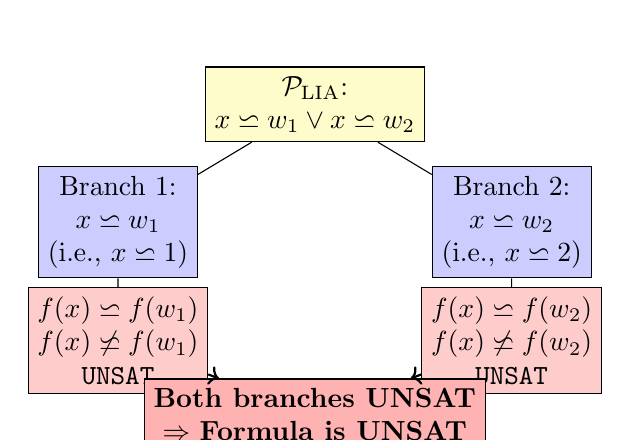
\begin{tikzpicture}[
    node distance=1.5cm and 2.5cm,
    every node/.style={align=center},
    level/.style={sibling distance=50mm/#1}
]
    \node[rectangle, draw, fill=yellow!20] (start) {$\mathcal{P}_{\text{LIA}}$: \\ $x \backsimeq w_1 \vee x \backsimeq w_2$}
        child {node[rectangle, draw, fill=blue!20] (b1) {Branch 1: \\ $x \backsimeq w_1$ \\ (i.e., $x \backsimeq 1$)}
            child {node[rectangle, draw, fill=red!20] (r1) {$f(x) \backsimeq f(w_1)$ \\ $f(x) \not\backsimeq f(w_1)$ \\ \texttt{UNSAT}}}}
        child {node[rectangle, draw, fill=blue!20] (b2) {Branch 2: \\ $x \backsimeq w_2$ \\ (i.e., $x \backsimeq 2$)}
            child {node[rectangle, draw, fill=red!20] (r2) {$f(x) \backsimeq f(w_2)$ \\ $f(x) \not\backsimeq f(w_2)$ \\ \texttt{UNSAT}}}};

    \node[rectangle, draw, fill=red!30, below=3cm of start] (final) {\textbf{Both branches UNSAT} \\ $\Rightarrow$ \textbf{Formula is UNSAT}};

    \draw[->,thick,dashed] (r1) -- (final);
    \draw[->,thick,dashed] (r2) -- (final);
\end{tikzpicture}
\end{center}

\vspace{0.5em}

\textbf{Contrast with $\mathcal{T}_{\text{LRA}}$}:

If we had used $\mathcal{T}_{\text{LRA}}$ (rationals) instead:
\begin{itemize}
    \item The constraint $1 \leq x \leq 2$ over rationals allows infinitely many values (e.g., $x = 1.5, 1.3, 1.7, \ldots$)
    \item The rational arithmetic procedure would \textbf{not} deduce $x \backsimeq 1 \vee x \backsimeq 2$
    \item No equality between shared variables would be propagated
    \item The procedures would terminate without finding a contradiction
    \item Result: \texttt{SAT} with assignment $x \leftarrow 1.5$ (or any value $\notin \{1, 2\}$ in the range)
\end{itemize}

This demonstrates the critical importance of \textbf{stable infiniteness} in theory combination: theories must agree on the cardinality of shared sorts, or unexpected results can occur.
\end{tcolorbox}
\end{example}

\newpage

\begin{example}[Non-Convex Theory: SAT with Three Branches]
\begin{tcolorbox}[colback=green!5!white,colframe=green!75!black,title=\textbf{Example 4: Non-Convex $\mathcal{T}_{\text{LIA}}$ — One SAT Branch Suffices},breakable]
\textbf{Given formula}:
\[
1 \leq x \quad \wedge \quad x \leq 3 \quad \wedge \quad f(x) \not\backsimeq f(1) \quad \wedge \quad f(x) \not\backsimeq f(3) \quad \wedge \quad f(1) \not\backsimeq f(2)
\]

\textbf{Question}: Is this formula satisfiable or unsatisfiable?

\vspace{0.5em}

\textbf{Key observation}: This example extends the previous one by allowing \textbf{three possible integer values} for $x$. Unlike Example 3, where both branches were UNSAT, here we will see that \textbf{one SAT branch is sufficient} to make the entire formula satisfiable.

\vspace{0.5em}

\textbf{Step 1: Identify the theories involved}

\begin{itemize}
    \item $\mathcal{T}_E$ (Theory of Equality with uninterpreted functions) — \textbf{convex}
    \item $\mathcal{T}_{\text{LIA}}$ (Linear Integer Arithmetic) — \textbf{non-convex}
\end{itemize}

\vspace{0.5em}

\textbf{Step 2: Separation Phase}

We separate the formula into $F_E$ and $F_{\text{LIA}}$:

\begin{align*}
F_E &: f(x) \not\backsimeq f(w_1) \quad \wedge \quad f(x) \not\backsimeq f(w_3) \quad \wedge \quad f(w_1) \not\backsimeq f(w_2) \\
F_{\text{LIA}} &: 1 \leq x \quad \wedge \quad x \leq 3 \quad \wedge \quad w_1 \backsimeq 1 \quad \wedge \quad w_2 \backsimeq 2 \quad \wedge \quad w_3 \backsimeq 3
\end{align*}

\textbf{Set of shared variables}:
\[
V = \{w_1, w_2, w_3, x\}
\]

\vspace{0.5em}

\textbf{Step 3: Deterministic Nelson-Oppen for Non-Convex Theories}

\textbf{Initial state}: $\mathcal{E}_0 = \emptyset$

\vspace{0.3em}

\textbf{Analysis by $\mathcal{P}_{\text{LIA}}$}:

The arithmetic procedure analyzes the constraints:
\[
1 \leq x \quad \wedge \quad x \leq 3
\]

Since $x$ is an integer and $1 \leq x \leq 3$, the only possible values are:
\[
\mathcal{P}_{\text{LIA}}: \{1 \leq x \wedge x \leq 3\} \models_{\mathcal{T}_{\text{LIA}}} x \backsimeq 1 \vee x \backsimeq 2 \vee x \backsimeq 3
\]

Equivalently, using shared variables:
\[
\mathcal{P}_{\text{LIA}} \text{ deduces: } x \backsimeq w_1 \vee x \backsimeq w_2 \vee x \backsimeq w_3
\]

\vspace{0.3em}

\textbf{Case Analysis}: We must explore all three branches:

\begin{itemize}
    \item \textbf{Branch 1}: $\mathcal{E}_1 = \{x \backsimeq w_1\}$ (i.e., $x \backsimeq 1$)
    \item \textbf{Branch 2}: $\mathcal{E}_2 = \{x \backsimeq w_2\}$ (i.e., $x \backsimeq 2$)
    \item \textbf{Branch 3}: $\mathcal{E}_3 = \{x \backsimeq w_3\}$ (i.e., $x \backsimeq 3$)
\end{itemize}

\vspace{0.5em}

\textbf{Step 4: Branch 1 — Assume $x \backsimeq w_1$ (i.e., $x \backsimeq 1$)}

The central manager sends $x \backsimeq w_1$ to both procedures.

\textbf{Analysis by $\mathcal{P}_E$}:

The congruence closure procedure receives $x \backsimeq w_1$ and processes:
\begin{align*}
x \backsimeq w_1 &\models_{\mathcal{T}_E} f(x) \backsimeq f(w_1) \quad \text{(by congruence)}
\end{align*}

But from $F_E$, we have:
\[
f(x) \not\backsimeq f(w_1)
\]

\textbf{Contradiction in Branch 1!}

We have both $f(x) \backsimeq f(w_1)$ and $f(x) \not\backsimeq f(w_1)$.

\textbf{Branch 1 result}: \texttt{UNSAT}

\vspace{0.5em}

\textbf{Step 5: Branch 3 — Assume $x \backsimeq w_3$ (i.e., $x \backsimeq 3$)}

The central manager sends $x \backsimeq w_3$ to both procedures.

\textbf{Analysis by $\mathcal{P}_E$}:

The congruence closure procedure receives $x \backsimeq w_3$ and processes:
\begin{align*}
x \backsimeq w_3 &\models_{\mathcal{T}_E} f(x) \backsimeq f(w_3) \quad \text{(by congruence)}
\end{align*}

But from $F_E$, we have:
\[
f(x) \not\backsimeq f(w_3)
\]

\textbf{Contradiction in Branch 3!}

We have both $f(x) \backsimeq f(w_3)$ and $f(x) \not\backsimeq f(w_3)$.

\textbf{Branch 3 result}: \texttt{UNSAT}

\vspace{0.5em}

\textbf{Step 6: Branch 2 — Assume $x \backsimeq w_2$ (i.e., $x \backsimeq 2$)}

The central manager sends $x \backsimeq w_2$ to both procedures.

\textbf{Analysis by $\mathcal{P}_E$}:

The congruence closure procedure receives $x \backsimeq w_2$ and processes:
\begin{align*}
x \backsimeq w_2 &\models_{\mathcal{T}_E} f(x) \backsimeq f(w_2) \quad \text{(by congruence)}
\end{align*}

Let's check the constraints in $F_E$:
\begin{itemize}
    \item $f(x) \not\backsimeq f(w_1)$ — Still satisfied (we have $f(w_2) \not\backsimeq f(w_1)$ or they could be different)
    \item $f(x) \not\backsimeq f(w_3)$ — Still satisfied (we have $f(w_2) \not\backsimeq f(w_3)$ or they could be different)
    \item $f(w_1) \not\backsimeq f(w_2)$ — This is explicitly required in $F_E$, so it's satisfied
\end{itemize}

\textbf{No contradiction in Branch 2!}

The congruence closure algorithm processes $F_E \cup \{x \backsimeq w_2\}$ and finds no inconsistency. The equality $f(x) \backsimeq f(w_2)$ does not conflict with any constraint in $F_E$.

Neither procedure can deduce any new equalities or contradictions.

\textbf{Branch 2 result}: \texttt{SAT}

\vspace{0.5em}

\textbf{Step 7: Final Verdict}

Since \textbf{at least one branch} is satisfiable (Branch 2), the formula is satisfiable.

\textbf{Key rule for non-convex theories}:
\begin{itemize}
    \item For the formula to be \texttt{UNSAT}: \textbf{ALL branches} must be \texttt{UNSAT}
    \item For the formula to be \texttt{SAT}: \textbf{At least ONE branch} must be \texttt{SAT}
\end{itemize}

\vspace{0.5em}

\textbf{Final Answer}: The formula is \texttt{SAT}.

\vspace{0.5em}

\textbf{Step 8: Satisfying Assignment}

We can construct a satisfying assignment based on Branch 2 ($x \backsimeq 2$):

\begin{align*}
x &\leftarrow 2 \\
w_1 &\leftarrow 1 \\
w_2 &\leftarrow 2 \\
w_3 &\leftarrow 3 \\
f(1) &\leftarrow \alpha \quad \text{(some value)} \\
f(2) &\leftarrow \beta \quad \text{(different from } \alpha \text{)} \\
f(3) &\leftarrow \gamma \quad \text{(any value)}
\end{align*}

\textbf{Verification}:
\begin{itemize}
    \item $1 \leq x \wedge x \leq 3$: $1 \leq 2 \leq 3$ \checkmark
    \item $f(x) \not\backsimeq f(1)$: $f(2) = \beta \neq \alpha = f(1)$ \checkmark
    \item $f(x) \not\backsimeq f(3)$: $f(2) = \beta$ can be different from $f(3) = \gamma$ \checkmark
    \item $f(1) \not\backsimeq f(2)$: $f(1) = \alpha \neq \beta = f(2)$ \checkmark
\end{itemize}

For example, we can set $\alpha = 10$, $\beta = 20$, $\gamma = 20$ (or any other values satisfying the disequalities).

\vspace{0.5em}

\textbf{Branching Visualization}:

\begin{center}
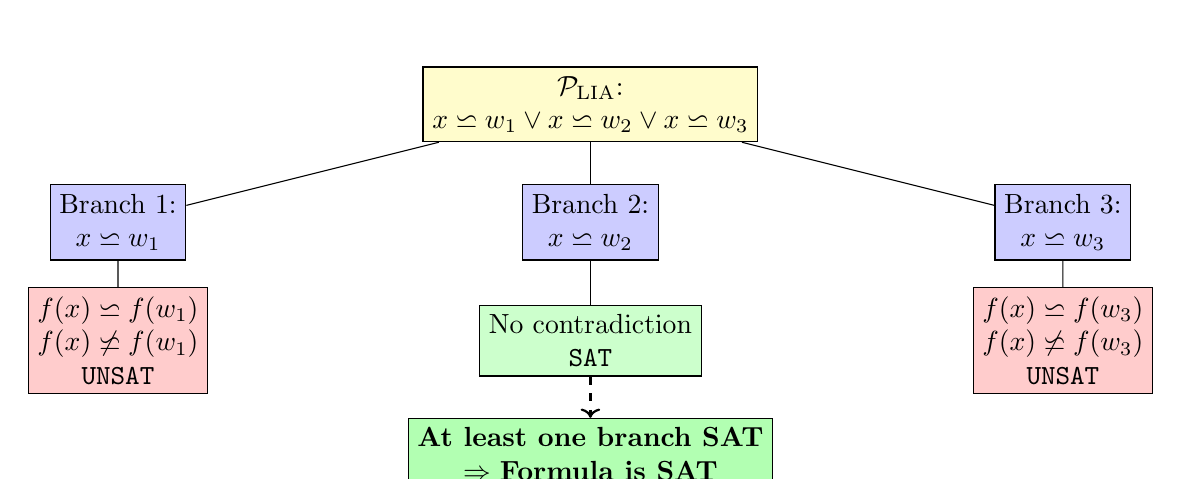
\begin{tikzpicture}[
    node distance=1.5cm and 2cm,
    every node/.style={align=center},
    level 1/.style={sibling distance=60mm},
    level 2/.style={sibling distance=30mm}
]
    \node[rectangle, draw, fill=yellow!20] (start) {$\mathcal{P}_{\text{LIA}}$: \\ $x \backsimeq w_1 \vee x \backsimeq w_2 \vee x \backsimeq w_3$}
        child {node[rectangle, draw, fill=blue!20] (b1) {Branch 1: \\ $x \backsimeq w_1$}
            child {node[rectangle, draw, fill=red!20] (r1) {$f(x) \backsimeq f(w_1)$ \\ $f(x) \not\backsimeq f(w_1)$ \\ \texttt{UNSAT}}}}
        child {node[rectangle, draw, fill=blue!20] (b2) {Branch 2: \\ $x \backsimeq w_2$}
            child {node[rectangle, draw, fill=green!20] (r2) {No contradiction \\ \texttt{SAT}}}}
        child {node[rectangle, draw, fill=blue!20] (b3) {Branch 3: \\ $x \backsimeq w_3$}
            child {node[rectangle, draw, fill=red!20] (r3) {$f(x) \backsimeq f(w_3)$ \\ $f(x) \not\backsimeq f(w_3)$ \\ \texttt{UNSAT}}}};

    \node[rectangle, draw, fill=green!30, below=3.5cm of start] (final) {\textbf{At least one branch SAT} \\ $\Rightarrow$ \textbf{Formula is SAT}};

    \draw[->,thick,dashed] (r2) -- (final);
\end{tikzpicture}
\end{center}

\vspace{0.5em}

\textbf{Key Insights}:

\begin{enumerate}
    \item This example demonstrates the \textbf{existential nature} of satisfiability in non-convex theories: we only need \textbf{one} satisfying assignment.

    \item The constraint $f(w_1) \not\backsimeq f(w_2)$ in $F_E$ is crucial: it prevents Branch 2 from having a contradiction because $f(2)$ is explicitly required to be different from $f(1)$.

    \item If the constraint $f(1) \not\backsimeq f(2)$ were not present, Branch 2 might still be SAT (depending on other constraints), but the reasoning would be different.

    \item This illustrates a practical strategy: when dealing with non-convex theories, the decision procedure must explore \textbf{all branches} until either:
    \begin{itemize}
        \item One branch is found to be \texttt{SAT} → return \texttt{SAT}
        \item All branches are found to be \texttt{UNSAT} → return \texttt{UNSAT}
    \end{itemize}
\end{enumerate}
\end{tcolorbox}
\end{example}

\newpage



\part{Beyond Conjunctions: Handling General Formulas}



\section{From Sets of Literals to General Formulas}



So far, we have studied decision procedures that work with \textbf{sets of literals} (conjunctions of atoms):



\begin{itemize}

    \item \textbf{Congruence Closure}: Handles sets of equality literals in $\mathcal{T}_E$

    \item \textbf{Theory of Lists/Constructors}: Handles sets of literals involving list operations

    \item \textbf{Theory of Arrays}: Handles sets of literals with $\textsf{select}$ and $\textsf{store}$

    \item \textbf{Nelson-Oppen}: Combines theories by sharing equalities between procedures

\end{itemize}



\begin{tcolorbox}[colback=yellow!10!white,colframe=orange!75!black,title=\textbf{Key Question}]

How do we handle more \textbf{general formulas} that contain \textbf{disjunctions}, not just conjunctions of literals?

\end{tcolorbox}



\subsection{The Challenge}



Most decision procedures are designed to work with \textbf{conjunctions} of literals:
\[
L_1 \wedge L_2 \wedge \cdots \wedge L_n
\]



But in practice, we often need to check satisfiability of formulas with complex Boolean structure:
\[
(L_1 \vee L_2) \wedge (L_3 \vee \neg L_4 \vee L_5) \wedge \cdots
\]



\subsection{Solution Approach: SAT Solver Integration}



The key idea is to combine:

\begin{enumerate}

    \item A \textbf{SAT solver} to handle the Boolean structure

    \item \textbf{Theory decision procedures} to handle the theory constraints

\end{enumerate}



This approach is known as \textbf{SMT (Satisfiability Modulo Theories)}.



\section{The Abstraction-Refinement Framework}



\subsection{Step 1: Convert to CNF}



Given a general first-order formula $F$, we first convert it to \textbf{Equisatisfiable Conjunctive Normal Form (ECNF)}:
\[
F \longrightarrow \text{ECNF} \longrightarrow S
\]



where $S$ is a \textbf{set of clauses} (CNF formula).



\begin{example}[CNF Conversion]

Original formula:
\[
f(x) \backsimeq y \rightarrow (x \backsimeq 1 \vee x \backsimeq 2)
\]

Convert to CNF:
\[
\neg(f(x) \backsimeq y) \vee x \backsimeq 1 \vee x \backsimeq 2
\]



This becomes a single clause:
\[
\{f(x) \not\backsimeq y, x \backsimeq 1, x \backsimeq 2\}
\]

\end{example}



\subsection{Step 2: Abstraction Function}



We define an \textbf{abstraction function} $\alpha$ that maps first-order atoms to propositional variables:



\begin{tcolorbox}[colback=blue!5!white,colframe=blue!75!black,title=\textbf{Abstraction Function}]
\[
\alpha: \text{First-order atoms} \longrightarrow \text{Propositional variables}
\]



\textbf{Examples}:
\begin{align*}
\alpha(f(x) \backsimeq y) &= P_1 \\
\alpha(x \backsimeq 1) &= P_2 \\
\alpha(x \backsimeq 2) &= P_3
\end{align*}



We also need the \textbf{inverse function}:
\[
\alpha^{-1}: \text{Propositional variables} \longrightarrow \text{First-order atoms}
\]

\textbf{Examples}:
\begin{align*}
\alpha^{-1}(P_1) &= f(x) \backsimeq y \\
\alpha^{-1}(P_2) &= x \backsimeq 1 \\
\alpha^{-1}(P_3) &= x \backsimeq 2
\end{align*}

\end{tcolorbox}



\subsection{Step 3: The SMT Architecture}



The integration between SAT solver and theory procedures works as follows:



\begin{center}
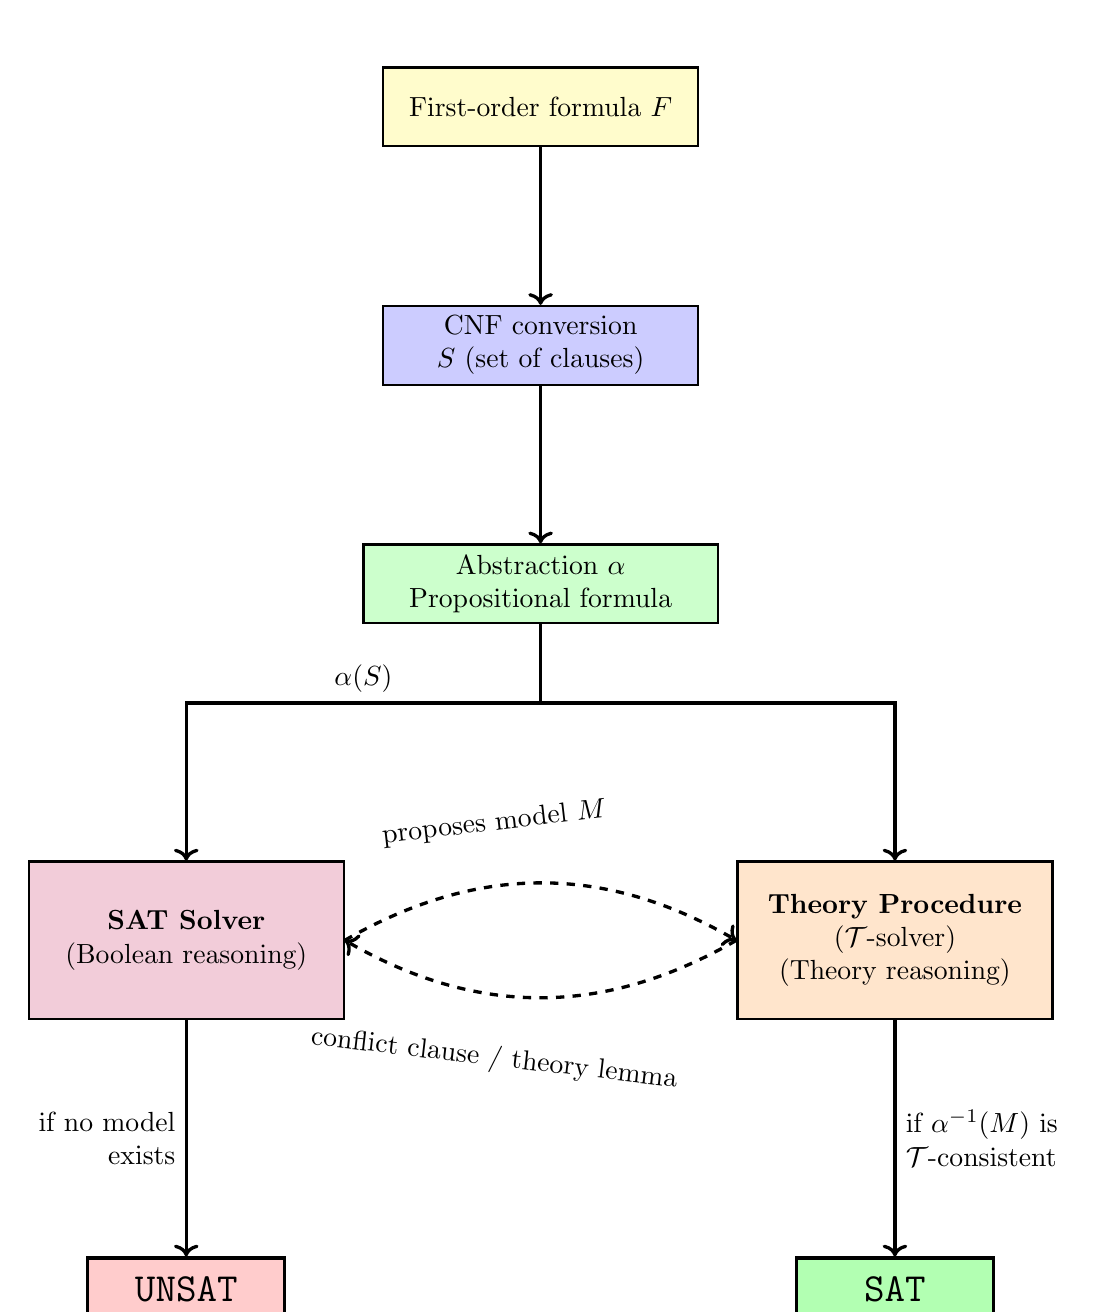
\begin{tikzpicture}[
    node distance=2cm,
    thick,
    box/.style={rectangle, draw, thick, minimum height=1cm, align=center},
    result/.style={rectangle, draw, very thick, minimum height=0.8cm, minimum width=2.5cm, align=center}
]
    % Top flow - centered
    \node[box, fill=yellow!20, minimum width=4cm] (F) {First-order formula $F$};
    \node[box, fill=blue!20, minimum width=4cm, below=of F] (CNF) {CNF conversion \\ $S$ (set of clauses)};
    \node[box, fill=green!20, minimum width=4.5cm, below=of CNF] (abs) {Abstraction $\alpha$ \\ Propositional formula};
    % SAT and Theory solvers side by side - properly centered using xshift
    \node[box, fill=purple!20, minimum width=4cm, minimum height=2cm, below=3cm of abs, xshift=-4.5cm] (sat) {\textbf{SAT Solver} \\ (Boolean reasoning)};
    \node[box, fill=orange!20, minimum width=4cm, minimum height=2cm, below=3cm of abs, xshift=4.5cm] (theory) {\textbf{Theory Procedure} \\ ($\mathcal{T}$-solver) \\ (Theory reasoning)};
    % Results at bottom - centered
    \node[result, fill=red!20, below=3cm of sat] (unsat) {\Large\texttt{UNSAT}};
    \node[result, fill=green!30, below=3cm of theory] (sat_result) {\Large\texttt{SAT}};
    % Arrows - preprocessing flow
    \draw[->, very thick] (F) -- (CNF);
    \draw[->, very thick] (CNF) -- (abs);
    \draw[->, very thick] (abs) |- ([yshift=-1cm]abs.south) -| node[near start, above] {$\alpha(S)$} (sat);
    \draw[->, very thick] (abs) |- ([yshift=-1cm]abs.south) -| (theory);
    % Interaction arrows
    \draw[->, dashed, very thick, bend left=30] (sat.east) to node[above, sloped, pos=0.4, yshift=5mm] {proposes model $M$} (theory.west);
    \draw[->, dashed, very thick, bend left=30] (theory.west) to node[below, sloped, pos=0.6, yshift=-5mm] {conflict clause / theory lemma} (sat.east);
    % Result arrows
    \draw[->, very thick] (sat) -- node[left, align=right] {if no model\\exists} (unsat);
    \draw[->, very thick] (theory) -- node[right, align=left] {if $\alpha^{-1}(M)$ is \\ $\mathcal{T}$-consistent} (sat_result);
\end{tikzpicture}
\end{center}



\vspace{0.5em}



\textbf{Key components}:

\begin{itemize}

    \item \textbf{SAT Solver}: Handles the Boolean/propositional structure

    \item \textbf{Theory Procedure}: Checks theory-level consistency

    \item \textbf{Interaction}: Iterative refinement through model proposals and conflict clauses

\end{itemize}



\subsection{Step 4: The SMT Loop}



The SMT solver operates in a loop:



\begin{enumerate}

    \item The \textbf{SAT solver} works on the abstracted (propositional) formula



    \item If SAT solver returns \texttt{UNSAT}: \\

    → The original formula is \texttt{UNSAT} (we're done)



    \item If SAT solver returns \texttt{SAT} and proposes a model $M$: \\

    → Apply $\alpha^{-1}$ to get a set of theory literals \\

    → Send these literals to the \textbf{theory procedure}



    \item The theory procedure checks if the literals are $\mathcal{T}$-consistent:

    \begin{itemize}

        \item If \texttt{SAT}: Return \texttt{SAT} (we found a satisfying assignment)

        \item If \texttt{UNSAT}: Generate a \textbf{conflict clause} and send it back to the SAT solver, which continues the search

    \end{itemize}

\end{enumerate}



\begin{example}[Abstraction in Action]

Consider the disjunction produced by a non-convex theory:
\[
x \backsimeq w_1 \vee x \backsimeq w_2 \vee x \backsimeq w_3
\]

We abstract this as:
\[
P_1 \vee P_2 \vee P_3
\]

where:
\begin{align*}
\alpha^{-1}(P_1) &= x \backsimeq w_1 \\
\alpha^{-1}(P_2) &= x \backsimeq w_2 \\
\alpha^{-1}(P_3) &= x \backsimeq w_3
\end{align*}



When the SAT solver decides that $P_1$ is true, we check if $x \backsimeq w_1$ is $\mathcal{T}_E$-consistent with the other constraints, and so on.

\end{example}



\newpage



\part{SMT and ATP}



\section{Theory Propagation and Conflict}



Instead of a simple generate-and-test approach, a tighter integration between the SAT solver and the theory solver is used, based on two main mechanisms: \textbf{theory propagation} and \textbf{theory conflict}.



Let's assume:

\begin{center}

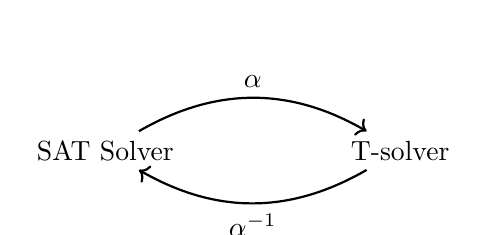
\begin{tikzpicture}[node distance=2cm, auto]

    \node (sat) {SAT Solver};

    \node (tsolver) [right=of sat, node distance=5cm] {T-solver};

    \draw[->, thick] (sat) to[bend left] node[above] {$\alpha$} (tsolver);

    \draw[->, thick] (tsolver) to[bend left] node[below] {$\alpha^{-1}$} (sat);

\end{tikzpicture}

\end{center}



\begin{itemize}

    \item \textbf{SAT Solver}: A tool that implements a procedure to decide the satisfiability of a set of clauses in propositional logic.

    \item \textbf{T-solver}: A tool that implements a procedure to decide the satisfiability of a set of $\mathcal{T}$-literals (e.g., for $\mathcal{T}_E, \mathcal{T}_{CONS}, \mathcal{T}_A$, or a combination).

    \item \textbf{$\alpha$}: The abstraction function that maps first-order atoms to propositional variables.

    \item \textbf{$\alpha^{-1}$}: The inverse of $\alpha$.

\end{itemize}



A tighter interaction involves two key ideas:



\begin{tcolorbox}[colback=blue!5!white,colframe=blue!75!black,title=\textbf{Theory Propagation}]

Assume we have the trail $\mathcal{M}$ (the current partial assignment) and the set of clauses $\mathcal{S}$ that we need to satisfy.
\[
\mathcal{M} \parallel \mathcal{S} \quad \longrightarrow \quad \mathcal{M}L_C \parallel \mathcal{S} \cup \{C\}
\]

if there exist literals $L_1, \dots, L_n \in \mathcal{M}$ such that $\{L_1, \dots, L_n\} \models_T L$, and $C = \neg L_1 \vee \dots \vee \neg L_n \vee L$. The atom of $L$ must occur in the input.

\end{tcolorbox}



\begin{tcolorbox}[colback=red!5!white,colframe=red!75!black,title=\textbf{Theory Conflict}]
\[
\mathcal{M} \parallel \mathcal{S} \quad \longrightarrow \quad \mathcal{M} \parallel \mathcal{S} \cup \{C\}
\]

if there are literals $L_1, \dots, L_n \in \mathcal{M}$ such that $\{L_1, \dots, L_n\}$ is $\mathcal{T}$-unsatisfiable (i.e., $\{L_1, \dots, L_n\} \models_T \bot$), and $C = \neg L_1 \vee \dots \vee \neg L_n$.

\end{tcolorbox}



With this, we conclude the part on satisfiability modulo theories.



\newpage



\part{Automated Theorem Proving in First-Order Logic}



\section{Dealing with Quantifiers}



We have seen satisfiability modulo theories, which covers:

\begin{itemize}

    \item Decision procedures for the satisfiability of sets of literals in single theories and in combination of theories.

    \item CDCL($\mathcal{T}$) to decide the satisfiability of ground clauses.

\end{itemize}

However, basic SMT methods do not handle quantifiers. Automated Theorem Proving (ATP) in first-order logic addresses this.



\textbf{Automated theorem proving in first-order logic}:

\begin{itemize}

    \item Involves quantifier reasoning.

    \item Basic ATP methods do not handle defined symbols other than equality, unless by adding the axioms defining the symbol to the input problem (e.g., for symbols a, b, c, f, g, h, ..., P, Q, R, ...).

\end{itemize}



\section{The ATP Problem and Skolemization}



The ATP problem is to determine if $H \models \phi$, which is equivalent to checking if $H \cup \{\neg \phi\}$ is unsatisfiable. The set of formulas is then converted to a clausal form $S$. The question is: is $S$ unsatisfiable?



A key issue in ATP is \textbf{Skolemization}, which does not preserve logical equivalence, but only equisatisfiability.

\begin{itemize}

    \item $\exists x F \longrightarrow F[x \leftarrow a]$ for $a$ a new constant symbol.

    \item $\forall y \exists x F \longrightarrow \forall y F[x \leftarrow f(y)]$ for $f$ a new function symbol.

\end{itemize}



\section{Herbrand Interpretations}



\subsection{Herbrand Universe}

The \textbf{Herbrand universe} $\mathcal{U}$ is the set of all ground terms in the signature of the input problem.

\begin{itemize}

    \item For $S = \{ P(a), \neg P(x) \vee P(f(x)) \}$, the Herbrand universe is $\mathcal{U} = \{ a, f(a), f(f(a)), \dots \} = \{ f^n(a) \mid n \geq 0 \}$.

    \item For $S = \{ P(a), \neg P(x) \vee P(f(x)), \neg R(x, y) \vee R(g(x, b), y) \}$, the Herbrand universe is $\mathcal{U} = \{ a, b, f(a), f(b), g(a, a), g(a, b), \dots \}$.

\end{itemize}



\subsection{Herbrand Base}

The \textbf{Herbrand base} $\mathcal{B}$ is the set of all ground atoms in the signature of the input problem.

\begin{itemize}

    \item For $S = \{ P(a), \neg Q(b), P(x) \vee \neg R(x) \}$, the Herbrand base is $\mathcal{B} = \{ P(a), P(b), Q(a), Q(b), R(a), R(b) \}$.

\end{itemize}



\subsection{Herbrand Interpretation}

A \textbf{Herbrand interpretation} $\mathcal{I}_H$ is an interpretation such that:

\begin{itemize}

    \item The domain $\mathcal{D}$ is the Herbrand universe $\mathcal{U}$.

    \item The interpretation function $\Phi$ is defined as:

    \begin{itemize}

        \item For all constant symbols $c$, $\Phi(c) = c$.

        \item For all function symbols $f$ of arity $n$, $\Phi(f)(t_1, \dots, t_n) = f(t_1, \dots, t_n)$.

    \end{itemize}

    \item A Herbrand interpretation is a subset of the Herbrand base, i.e., $\mathcal{I}_H \subseteq \mathcal{B}$. It is the set of all ground atoms that it makes true.

\end{itemize}

For example, for $S = \{ \neg P(x) \vee \neg P(f(x)) \}$, if we add a constant symbol $a$, the Herbrand Universe is $\mathcal{U} = \{ f^n(a) \mid n \geq 0 \}$. An interpretation that satisfies this clause over the natural numbers $\mathbb{N}$ could be $\mathcal{I} = \langle \mathbb{N}, \Phi \rangle$ where $\Phi(f)(n) = n+1$ and $\Phi(P) = \{ 2k \mid k \in \mathbb{N} \}$.

This is because $P(x) \rightarrow \neg P(f(x))$.



\subsection{Associated Herbrand Interpretation}

Given an interpretation $\mathcal{I}$, the associated Herbrand interpretation $\mathcal{I}_H$ is defined as $\mathcal{I}_H = \{ L \mid L \text{ is a ground literal and } \mathcal{I} \models L \}$.

The Herbrand interpretation $\mathcal{I}_H$ for a given interpretation $\mathcal{I}$ is unique unless we had to add a constant symbol.



For $S = \{ \neg P(x) \vee \neg P(f(x)) \}$, with no constant symbol, we add a new constant $a$. $\mathcal{U} = \{f^n(a) \mid n \ge 0\}$.

An interpretation satisfying this clause is $\mathcal{I} = \langle \mathbb{N}, \Phi \rangle$ with $\Phi(f)(n) = n+1$ and $\Phi(P) = \{2k \mid k \in \mathbb{N} \}$.

There exist two Herbrand interpretations associated to $\mathcal{I}$:

\begin{itemize}

    \item $\mathcal{I}_H^1 = \{ P(a), \neg P(f(a)), P(f^2(a)), \dots \} = \{ P(f^n(a)) \mid n=2k \} \cup \{ \neg P(f^n(a)) \mid n=2k+1 \}$

    \item $\mathcal{I}_H^2 = \{ \neg P(a), P(f(a)), \neg P(f^2(a)), \dots \} = \{ \neg P(f^n(a)) \mid n=2k \} \cup \{ P(f^n(a)) \mid n=2k+1 \}$

\end{itemize}



\subsection{Herbrand's Theorem}

\begin{itemize}

    \item Let $F$ be a formula and $S$ its clausal form.

    \item If $\mathcal{I} \models F$, then $\mathcal{I}_H \models S$ for all associated Herbrand interpretations $\mathcal{I}_H$.

    \item A set of clauses $S$ is unsatisfiable if and only if it is false in all Herbrand interpretations.

    ($\Rightarrow$) Trivial.

    ($\Leftarrow$) By contradiction: assume $\mathcal{I} \models S$. Then $\mathcal{I}_H \models S$, which is a contradiction.

\end{itemize}



\newpage



\part{Fundamentals of Theorem Proving}

\section{Introduction}

Automated theorem proving in first-order logic aims to mechanically determine whether a given formula is a logical consequence of a set of axioms. This is fundamentally different from the decision procedures we have studied for specific theories (such as equality or linear arithmetic), as first-order logic with quantifiers is only semi-decidable.

\section{Proof Procedures}

A \textbf{semi-decision procedure} for unsatisfiability in First-Order Logic (FOL) is called a \textbf{theorem-proving strategy} or \textbf{proof procedure}. Unlike decision procedures, which always terminate with a definite answer, a semi-decision procedure is guaranteed to terminate only when the input is unsatisfiable.

\begin{tcolorbox}[colback=yellow!5!white,colframe=yellow!75!black,title=\textbf{Semi-Decidability of First-Order Logic}]
\textbf{Key Properties}:
\begin{itemize}
    \item If a formula is \textbf{unsatisfiable}, the procedure will eventually detect this and terminate with "UNSAT"
    \item If a formula is \textbf{satisfiable}, the procedure may run forever without reaching a conclusion
    \item This asymmetry is inherent to first-order logic (consequence of Church-Turing undecidability results)
\end{itemize}
\end{tcolorbox}

\subsection{Structure of a Proof Procedure}

Every proof procedure consists of two essential components that work together to explore the space of possible proofs.

\begin{tcolorbox}[colback=blue!5!white,colframe=blue!75!black,title=\textbf{Components of a Proof Procedure}]
A proof procedure $P$ can be formally described as an ordered pair:
\[ P = \langle I, E \rangle \]
where:
\begin{itemize}
    \item $I$: \textbf{Inference System} --- A set of inference rules that define valid logical deductions

    \textit{Examples}: Resolution, Paramodulation, Superposition

    \item $E$: \textbf{Search Plan} (or \textbf{Search Strategy}) --- The strategy used to select which inference rules to apply and in what order

    \textit{Examples}: Breadth-first search, set-of-support strategy, ordered resolution
\end{itemize}
\end{tcolorbox}

\textbf{Design considerations}:
\begin{enumerate}
    \item The inference system must be \textbf{sound} (derive only valid consequences) and \textbf{refutation-complete} (able to derive a contradiction from any unsatisfiable set)
    \item The search plan must be \textbf{fair} (eventually consider all possible inferences) to ensure completeness
    \item Practical efficiency requires careful design of the search strategy to avoid exploring irrelevant parts of the search space
\end{enumerate}



\section{Herbrand's Theorem}

The fundamental problem in Automated Reasoning is determining whether a set of clauses $S$ is unsatisfiable (a logical contradiction). Herbrand's Theorem bridges the gap between general unsatisfiability and unsatisfiability within a restricted domain---the Herbrand universe.

\subsection{Statement of Herbrand's Theorem}

Herbrand's Theorem is one of the most important results in automated theorem proving. It justifies the approach of reasoning about first-order formulas using only ground terms.

\begin{tcolorbox}[colback=green!5!white,colframe=green!75!black,title=\textbf{Herbrand's Theorem}]
\begin{theorem}[Herbrand's Theorem]
A set of clauses $S$ is unsatisfiable if and only if $S$ is \textbf{H-unsatisfiable}, meaning $S$ is unsatisfiable under all Herbrand interpretations.
\end{theorem}
\end{tcolorbox}

\textbf{Significance}: This theorem allows us to restrict our attention to Herbrand interpretations when checking unsatisfiability. Instead of considering all possible interpretations over arbitrary domains, we only need to consider interpretations over the Herbrand universe (the set of all ground terms).

\subsection{Refined Herbrand's Theorem}

The refined version of Herbrand's Theorem is even more powerful for practical theorem proving, as it guarantees the existence of a \textit{finite} witness for unsatisfiability.

\begin{tcolorbox}[colback=blue!5!white,colframe=blue!75!black,title=\textbf{Refined Herbrand's Theorem}]
\begin{theorem}[Refined Herbrand's Theorem]
A set of clauses $S$ is unsatisfiable if and only if there exists a \textbf{finite} set $S'$ of ground instances of clauses in $S$ such that $S'$ is unsatisfiable.
\end{theorem}
\end{tcolorbox}

\textbf{Implications for theorem proving}:
\begin{enumerate}
    \item This theorem provides a semi-decision procedure: systematically generate ground instances and check for propositional unsatisfiability
    \item If $S$ is unsatisfiable, we will eventually find a finite unsatisfiable subset of ground instances
    \item If $S$ is satisfiable, the procedure may generate ground instances indefinitely
    \item This is the theoretical foundation for many automated theorem provers
\end{enumerate}



\subsection{The "Clause" Constraint \& Counter-Example}

It is crucial that Herbrand's Theorem applies specifically to \textbf{clauses} (formulas in conjunctive normal form with implicit universal quantification) and \textit{not} to arbitrary formulas containing existential quantifiers. This restriction is essential for the theorem's validity.

\begin{tcolorbox}[colback=red!5!white,colframe=red!75!black,title=\textbf{Important Restriction}]
Herbrand's Theorem requires the input to be in \textbf{clause normal form} (CNF). For formulas with existential quantifiers, Skolemization must be applied first to eliminate existential quantifiers before applying Herbrand's Theorem.
\end{tcolorbox}

The following counter-example demonstrates why this restriction is necessary.



\begin{example}[Counter-Example]

Consider the set $S = \{ \exists x P(x), \neg P(a) \}$.

\begin{itemize}

    \item \textbf{Analysis in the Herbrand universe (H):}

    \begin{itemize}

        \item Universe: $\mathcal{U}_H = \{a\}$

        \item Base: $\mathcal{B}_H = \{P(a)\}$

        \item Possible Herbrand interpretations:

        \begin{enumerate}

            \item $I = \emptyset$: $\neg P(a)$ is true. $\exists x P(x)$ fails (since $P(a)$ is false).

            \item $I = \{ P(a) \}$: $\neg P(a)$ is false.

        \end{enumerate}

        Result: $S$ is H-unsatisfiable.

    \end{itemize}

    \item \textbf{Analysis in general interpretations ($\mathcal{M}$):}

    Consider a model $\mathcal{M} = \langle D, I \rangle$ with:

    \begin{itemize}

        \item $D = \{1, 2\}$

        \item $I(a) = 1$

        \item $I(P) = \{2\}$

    \end{itemize}

    Then $\neg P(a)$ is true (since $1 \notin I(P)$) and $\exists x P(x)$ is true (since $2 \in I(P)$).

    Result: $S$ is satisfiable.

\end{itemize}

Conclusion: H-unsatisfiability only implies general unsatisfiability if the formula is in clause normal form (Skolemized).

\end{example}



\subsection{Practical Demonstrations}



\begin{example}[Proof of Validity]

\textbf{Problem}: Demonstrate that $F = \forall x A(x) \rightarrow A(b)$ is valid.



\textbf{Method}: Proof by refutation (show $\neg F$ is unsatisfiable).



\begin{enumerate}

    \item \textbf{Negation and CNF}:

    $\neg F = \neg (\forall x A(x) \rightarrow A(b)) \equiv \forall x A(x) \wedge \neg A(b)$.

    Clauses $S$: $\{A(x)\}, \{\neg A(b)\}$.

    \item \textbf{Universe and Base}:

    Herbrand Universe $\mathcal{U}_H = \{b\}$, Herbrand Base $\mathcal{B}_H = \{A(b)\}$.

    \item \textbf{Analysis of Interpretations}:

    \begin{itemize}

        \item If $I = \emptyset$: $A(b)$ is false. Clause $A(x)$ (grounded to $A(b)$) is falsified.

        \item If $I = \{A(b)\}$: $A(b)$ is true. Clause $\{\neg A(b)\}$ is falsified.

    \end{itemize}

    \item \textbf{Conclusion}: The set of ground instances $\{A(b), \neg A(b)\}$ is contradictory. Thus, $\neg F$ is unsatisfiable, and $F$ is valid.

\end{enumerate}

\end{example}



\begin{example}[Satisfiability Check]

\textbf{Problem}: Determine if $S' = \{P(b), \neg P(a)\}$ is satisfiable.

\begin{itemize}

    \item Universe $\mathcal{U} = \{a, b\}$

    \item Base $\mathcal{B} = \{P(a), P(b)\}$

\end{itemize}

\textbf{Analysis}: We look for an interpretation $I \subseteq \mathcal{B}$ that satisfies both clauses.

Let the interpretation be $I = \{P(b)\}$. Then $P(a)$ is false.

\begin{itemize}

    \item $P(b)$ is true.

    \item $\neg P(a)$ is true.

\end{itemize}

Result: $S'$ is satisfiable.

\end{example}



\subsection{Formal Mechanics: Substitutions and Grounding}

To rigorously apply Herbrand's theorem, we rely on substitutions to create ground instances.



\begin{definition}[Substitution]

A substitution $\sigma$ is a map from variables to terms, different from the identity only on a finite set of variables (the domain).

\[ \sigma = \{ x_1 \leftarrow t_1, \dots, x_n \leftarrow t_n \} \]

Constraints:

\begin{itemize}

    \item $x_i \neq x_j$ for $i \neq j$ (distinct variables).

    \item $x_i \neq t_i$ (no circular trivial assignments).

\end{itemize}

\end{definition}



\begin{example}

$\sigma = \{ x \leftarrow a, y \leftarrow b, z \leftarrow f(a), w \leftarrow g(x), v \leftarrow f(x') \}$.

(Note: $a, b$ are constants: f, g are functions; x, y, z, w, v, x' are variables).

\end{example}



\subsubsection{Application of Substitution}

Application of a substitution $\sigma$ to a term $t$, denoted $t\sigma$:
\[
t\sigma = \begin{cases}
    s & \text{if } t \text{ is a variable } x \in \text{Dom}(\sigma) \text{ and } (x \leftarrow s) \in \sigma \\
    t & \text{if } t \text{ is a variable } y \notin \text{Dom}(\sigma) \\
    c & \text{if } t \text{ is a constant } c \\
    f(t_1\sigma, \dots, t_n\sigma) & \text{if } t = f(t_1, \dots, t_n)
\end{cases}
\]

Application to literals and clauses:
\begin{itemize}
    \item Literal: $L\sigma = P(t_1\sigma, \dots, t_n\sigma)$
    \item Clause: $C\sigma = L_1\sigma \lor \dots \lor L_k\sigma$
\end{itemize}



\subsubsection{Grounding and Satisfaction}

A \textbf{Ground Instance} of a clause $C$ is a substituted clause $C\sigma$ that contains no variables.



\textbf{Satisfaction Criteria}:

\begin{enumerate}

    \item \textbf{Clause Satisfaction}: A Herbrand interpretation $\mathcal{I}_H$ satisfies a clause $C$ if $\mathcal{I}_H$ satisfies all ground instances of $C$.

    \item \textbf{Ground Instance Satisfaction}: $\mathcal{I}_H$ satisfies a ground clause $C\sigma = L_1\sigma \lor \dots \lor L_k\sigma$ if it satisfies at least one literal $L_i\sigma$.

\end{enumerate}



\begin{example}[Grounding Sequence]

Consider $C = \neg P(x) \lor P(f(x))$ and Universe $\mathcal{U} = \{a, f(a), f^2(a), \dots\}$.

\begin{itemize}

    \item $\sigma_0 = \{x \leftarrow a\} \implies C\sigma_0 = \neg P(a) \lor P(f(a))$

    \item $\sigma_1 = \{x \leftarrow f(a)\} \implies C\sigma_1 = \neg P(f(a)) \lor P(f^2(a))$

    \item \dots

    \item $\sigma_n = \{x \leftarrow f^n(a)\} \implies C\sigma_n = \neg P(f^n(a)) \lor P(f^{n+1}(a))$

\end{itemize}

For $\mathcal{I}_H$ to satisfy the original clause $C$, it must satisfy every instance in this infinite sequence.

\end{example}



\newpage



\part{Theorem Proving Strategies}

\section{Introduction to Theorem-Proving Strategies}

A \textbf{proof procedure} or \textbf{theorem-proving strategy} is a systematic method for determining the unsatisfiability of sets of first-order clauses. Each strategy consists of two key components that work together to explore the search space of possible proofs.

\begin{tcolorbox}[colback=blue!5!white,colframe=blue!75!black,title=\textbf{Structure of a Proof Procedure}]
\begin{definition}[Proof Procedure]
A proof procedure $P$ is formally described as an ordered pair:
\[ P = \langle I, \Sigma \rangle \]
where:
\begin{itemize}
    \item $I$: \textbf{Inference System} --- A set of inference rules that define valid logical deductions (e.g., Resolution, Paramodulation)
    \item $\Sigma$: \textbf{Search Plan} --- The strategy used to explore the search space and select which inferences to apply
\end{itemize}
\end{definition}
\end{tcolorbox}

The effectiveness of a proof procedure depends on both components: the inference system must be sound and complete, while the search plan must efficiently guide the proof search.

\section{Families of Theorem-Proving Strategies}

Theorem-proving strategies can be broadly classified into two main families, each with distinct approaches to handling first-order formulas.

\subsection{Instance-Based Strategies}

\textbf{Instance-based strategies} operate by generating ground instances of clauses and reducing the first-order problem to propositional logic.

\begin{tcolorbox}[colback=green!5!white,colframe=green!75!black,title=\textbf{Instance-Based Approach}]
These strategies:
\begin{itemize}
    \item Define inference rules to systematically generate ground instances of clauses
    \item Follow a scheme that directly implements Herbrand's Theorem
    \item Reduce the First-Order Logic problem to a sequence of propositional satisfiability problems
    \item Use SAT solvers to check the satisfiability of the generated ground instances
\end{itemize}

\textbf{Key advantage}: Leverages efficient propositional SAT solving techniques.

\textbf{Examples}: DPLL(T), SMT solvers with instantiation.
\end{tcolorbox}

The process can be visualized as follows: given a set of first-order clauses $S$, the strategy generates an increasing sequence of ground instances $S_0 \subseteq S_1 \subseteq S_2 \subseteq \cdots$ until either:
\begin{enumerate}
    \item A contradiction is found in some $S_i$ (proving unsatisfiability), or
    \item The procedure continues indefinitely (which may happen for satisfiable sets)
\end{enumerate}

\subsection{Ordering-Based Strategies}

\textbf{Ordering-based strategies} work directly with first-order clauses without necessarily grounding them.

\begin{tcolorbox}[colback=orange!5!white,colframe=orange!75!black,title=\textbf{Ordering-Based Approach}]
These strategies:
\begin{itemize}
    \item Define inference rules that operate directly on First-Order clauses
    \item Instantiate variables in clauses through \textbf{matching} or \textbf{unifying} substitutions
    \item Use term orderings to guide and restrict inference steps
    \item Generate new clauses by combining existing clauses according to inference rules
\end{itemize}

\textbf{Key advantage}: More general, can handle infinite domains without explicit grounding.

\textbf{Examples}: Resolution, Superposition, Paramodulation.
\end{tcolorbox}

The distinction between these two families is fundamental: instance-based strategies explicitly enumerate ground terms, while ordering-based strategies manipulate first-order clauses symbolically.

\section{Substitutions}

Substitutions are the fundamental mechanism for instantiating variables in first-order logic. They play a central role in both families of theorem-proving strategies.

\subsection{Basic Definition}

\begin{tcolorbox}[colback=purple!5!white,colframe=purple!75!black,title=\textbf{Substitution}]
\begin{definition}[Substitution]
A \textbf{substitution} is a mapping from variables to terms:
\[ \alpha: X \to T(\mathcal{F}, X) \]
where:
\begin{itemize}
    \item $X$ is the set of variables
    \item $T(\mathcal{F}, X)$ is the set of terms over function symbols $\mathcal{F}$ and variables $X$
\end{itemize}

A substitution differs from the identity mapping on only a \textbf{finite} set of variables.
\end{definition}
\end{tcolorbox}

\textbf{Notation}: A substitution is typically written as a finite set of variable-term pairs:
\[ \alpha = \{ x_1 \leftarrow t_1, \dots, x_n \leftarrow t_n \} \]
where each $x_i$ is a variable and each $t_i$ is a term. This means that $\alpha(x_i) = t_i$ for $i = 1, \dots, n$, and $\alpha(x) = x$ for all other variables $x \notin \{x_1, \dots, x_n\}$.

\subsection{Components of a Substitution}

Every substitution has two important associated sets:

\begin{itemize}
    \item \textbf{Domain}: $\text{Dom}(\alpha) = \{ x_1, \dots, x_n \}$ --- the set of variables that are mapped to different terms
    \item \textbf{Rank}: $\text{Rank}(\alpha) = \bigcup_{i=1}^{n} \text{Var}(t_i)$ --- the set of all variables appearing in the target terms, where $\text{Var}(t_i)$ denotes the set of variables occurring in term $t_i$
\end{itemize}

\subsection{Idempotent Substitutions}

A special class of substitutions that behave particularly well under repeated application are the idempotent substitutions.

\begin{tcolorbox}[colback=red!5!white,colframe=red!75!black,title=\textbf{Idempotence}]
\begin{definition}[Idempotent Substitution]
A substitution $\alpha$ is \textbf{idempotent} if and only if:
\[ \text{Dom}(\alpha) \cap \text{Rank}(\alpha) = \emptyset \]

Equivalently, $\alpha$ is idempotent if applying it twice gives the same result as applying it once: $\alpha\alpha = \alpha$.
\end{definition}
\end{tcolorbox}

\textbf{Intuition}: An idempotent substitution does not map any variable to a term containing variables in its domain. This ensures that once applied, no further changes occur.

\begin{example}[Non-Idempotent Substitution]
Consider the substitution $\alpha = \{x \leftarrow f(y), y \leftarrow c\}$.

\textbf{Analysis}:
\begin{itemize}
    \item $\text{Dom}(\alpha) = \{x, y\}$
    \item $\text{Rank}(\alpha) = \text{Var}(f(y)) \cup \text{Var}(c) = \{y\} \cup \emptyset = \{y\}$
    \item $\text{Dom}(\alpha) \cap \text{Rank}(\alpha) = \{x, y\} \cap \{y\} = \{y\} \neq \emptyset$
\end{itemize}

Therefore, $\alpha$ is \textbf{not idempotent}.

\textbf{Demonstration}: Applying $\alpha$ to $x$:
\begin{align*}
x\alpha &= f(y) \\
(x\alpha)\alpha &= f(y)\alpha = f(y\alpha) = f(c)
\end{align*}

Since $x\alpha \neq (x\alpha)\alpha$, we confirm that $\alpha$ is not idempotent. The substitution continues to have effect when applied repeatedly because the domain variable $y$ appears in the range of the substitution.
\end{example}

\begin{remark}
Idempotent substitutions are important in automated reasoning because they simplify the theoretical analysis and implementation of unification algorithms. Many theorem provers normalize substitutions to idempotent form to avoid the complications of repeated application.
\end{remark}



\newpage

\iffalse % WIP draft — un-comment when finished

\part{}

\section{}

We have seen substitutions \sigma
We are interested in Idempotent substitutions: one such that
forall i, j 1 <= i, j <= n    x_i not in Var(t_j)     Dom(\sigma) not intersected with Rank(\alpha)

where Var(t_j) are the variables in t_j 

if we apply substitution twice, we get the same result as applying it once 

we define Composition of substitutions \Theta = { y <-- s_1, ..., y_m <-- s_m }
How do we define \sigma composition \Theta?
t(\sigma \dot \Theta) = (t\sigma)\Theta 

\sigma \dot \Theta = { x_1 <-- t_1\Theta, x_2 <-- t_2\Theta, ..., x_n <-- t_n\Theta | x_i =/= t_1\Theta 1 <= i <= n } U { y_j <-- s_j | y_j not in Dom(\sigma) }




\section{}

How are we going to use these substitutions?

Two uses of substitution in interence rules:
1) Matching substitutions    t\sigma = s     s is an instance of t 
t = f(x, y)     s = f(a, b)
\sigma = { x <-- a, y <-- b }

2) Unifying substitution or unifier:     s\sigma = t\sigma
P(x, b)     P(z, y)
\sigma = { x <-- z, y <-- b } is the common instance 
\sigma = { z <-- x, y <-- b } "   "    "     "


Unification problem: E = { s_i =?= t_i }^n _{i = 1}

Solution (a unifier): substitution \sigma such that s_i\sigma = t_i\sigma forall i 1 <= i <= n 

Better solution: a most general unifier 

most general:

\sigma <= (more general, with a dot inside) \Theta if E \rho \sigma \dot \rho = \Theta    \sigma is more general than \Theta

\sigma <= \Theta if \sigma <= \Theta and \Theta </= \sigma



Variable renaming: it's a substitution that maps variables to variables and is injective.



So, known this, what is a most general unifier?

A most general unifier is a substitution \sigma which is a unifier and for all other unifiers \Theta it is \sigma more general than \Theta.

The most general unifier (m.g.u.) is unique up to variable renaming (i.e., if there are two MGUs \sigma_1 and \sigma_2, then they are in disequivalence relation because one is more general than the other).


How to compute a MGU --> there are algorithms, in particolar Robinson's algorithm.

Robinson's Algorithm: it procudes an idempotent most general unifier
(explain)

\fi % end WIP draft

\end{document}
